%%%%%%%%%%%%%%%%%%%%%%%%%%%%%%%%%%%%%%%%%%%%%%%%%%%%%%%%%%%%%%%%%%%%%%%%%%%%%
%%%% Preamble
%%%%%%%%%%%%%%%%%%%%%%%%%%%%%%%%%%%%%%%%%%%%%%%%%%%%%%%%%%%%%%%%%%%%%%%%%%%%%

%%%% The uwthesis.sty file relies on the memoir class!
%%%% You should be using the memoir class anyway; it makes life easier:
%%%% http://www.ctan.org/tex-archive/macros/latex/contrib/memoir/


%\RequirePackage{lineno}
\documentclass[oneside, letterpaper, 12pt, oldfontcommands]{memoir}


\setsecnumdepth{subsubsection}

% Package imports and other setup
\usepackage{includes/uwthesis}
\usepackage{graphicx}
\usepackage{amsfonts}
\usepackage{mathrsfs}
\usepackage{amsmath}
\usepackage{textcomp}
\usepackage{gensymb}
\usepackage{xspace}
\usepackage[utf8]{inputenc}
\usepackage[hidelinks]{hyperref}
\usepackage[
  sorting=none,
  backend=biber,
  style=ieee
]{biblatex}

\hypersetup{
  colorlinks,
  allcolors=black
}

\setsecnumdepth{subsubsection}
\maxtocdepth{subsubsection}

% Collaboration instead of author if present
\DeclareSourcemap{
  \maps[datatype=bibtex,overwrite=true]{
    \map{
      \step[fieldsource=collaboration,% fieldvalue={$1 Collaboration},
            final=true]
      \step[fieldset=usera, origfieldval, final=true]
    }
  }
}
\renewbibmacro*{author}{
  \iffieldundef{usera}{
    \printnames{author}
  }{
      \printfield{usera} Collaboration
  }
}


% command for changing IEEE bib format
%\makeatletter
%\def\bstctlcite{\@ifnextchar[{\@bstctlcite}{\@bstctlcite[@auxout]}}
%\def\@bstctlcite[#1]#2{\@bsphack
%  \@for\@citeb:=#2\do{%
%    \edef\@citeb{\expandafter\@firstofone\@citeb}%
%    \if@filesw\immediate\write\csname %#1\endcsname{\string\citation{\@citeb}}\fi}%
%  \@esphack}
%\makeatother

% packages I don't need now, but which might be useful later
%\usepackage{mathtools}
%\usepackage{subfig}
%\usepackage{caption}
%\usepackage{subcaption}
%\usepackage{adjustbox}
%\usepackage{xr}
%\usepackage{ifthen}
%\usepackage{multirow}
%\usepackage{feynmp-auto}
%\usepackage{tikz}
%\usetikzlibrary{arrows}
%\usepackage{pdflscape}

% Symbols and a few functions

\usepackage{amsmath}


\newcommand{\cmsSymbolFace}{\mathrm}

% particles
\newcommand{\Pe}{\ensuremath{\cmsSymbolFace{e}}\xspace}
\newcommand{\Pm}{\ensuremath{\cmsSymbolFace{\mu}}\xspace}
\newcommand{\Pt}{\ensuremath{\cmsSymbolFace{\tau}}\xspace}
\newcommand{\PW}{\ensuremath{\cmsSymbolFace{W}}\xspace}
\newcommand{\PWp}{\ensuremath{\cmsSymbolFace{W}^+}\xspace}
\newcommand{\PWm}{\ensuremath{\cmsSymbolFace{W}^-}\xspace}
\newcommand{\PZ}{\ensuremath{\cmsSymbolFace{Z}}\xspace}
\newcommand{\PH}{\ensuremath{\cmsSymbolFace{H}}\xspace}
\newcommand{\PV}{\ensuremath{\cmsSymbolFace{V}}\xspace}
\newcommand{\Pa}{\ensuremath{\cmsSymbolFace{\gamma}}\xspace}
\newcommand{\Pg}{\ensuremath{\cmsSymbolFace{g}}\xspace}
\newcommand{\Pp}{\ensuremath{\cmsSymbolFace{p}}\xspace}
\newcommand{\Pq}{\ensuremath{\cmsSymbolFace{q}}\xspace}
\newcommand{\Pqt}{\ensuremath{\cmsSymbolFace{t}}\xspace}
\newcommand{\Pqb}{\ensuremath{\cmsSymbolFace{b}}\xspace}
\newcommand{\Paq}{\ensuremath{\bar{\cmsSymbolFace{q}}}\xspace}
\newcommand{\Paqt}{\ensuremath{\bar{\cmsSymbolFace{t}}}\xspace}
\newcommand{\Paqb}{\ensuremath{\bar{\cmsSymbolFace{b}}}\xspace}
\newcommand{\Plp}{\ensuremath{\ell^+}\xspace}
\newcommand{\Plm}{\ensuremath{\ell^-}\xspace}
\newcommand{\Plpp}{\ensuremath{\ell'^+}\xspace}
\newcommand{\Plpm}{\ensuremath{\ell'^-}\xspace}
% unknown particle
\newcommand{\PX}{\ensuremath{\cmsSymbolFace{X}}\xspace}

% multiple particles
\newcommand{\ZZ}{\ensuremath{\PZ\PZ}\xspace}
\newcommand{\WZ}{\ensuremath{\PW\PZ}\xspace}
\newcommand{\WW}{\ensuremath{\PW\PW}\xspace}
\newcommand{\ZA}{\ensuremath{\PZ\Pa}\xspace}
\newcommand{\VVV}{\ensuremath{\PV\PV\PV}\xspace}
\newcommand{\ZZZ}{\ensuremath{\PZ\PZ\PZ}\xspace}
\newcommand{\WWZ}{\ensuremath{\PW\PW\PZ}\xspace}
\newcommand{\VH}{\ensuremath{\PV\PH}\xspace}
\newcommand{\TTbar}{\ensuremath{\Pqt\Paqt}\xspace}
\newcommand{\TTV}{\ensuremath{\Pqt\Paqt\PV}\xspace}
\newcommand{\TTZ}{\ensuremath{\Pqt\Paqt\PZ}\xspace}
\newcommand{\TTW}{\ensuremath{\Pqt\Paqt\PW}\xspace}
\newcommand{\pp}{\ensuremath{\Pp\Pp}\xspace}
\newcommand{\llll}{\ensuremath{4\ell}\xspace}
\newcommand{\eeee}{\ensuremath{4\Pe}\xspace}
\newcommand{\eemm}{\ensuremath{2\Pe2\Pm}\xspace}
\newcommand{\mmmm}{\ensuremath{4\Pm}\xspace}
\newcommand{\lplmlplm}{\ensuremath{\Plp\Plm\Plpp\Plpm}\xspace}

% generators and similar
\newcommand{\FEWZ} {{\textsc{fewz}}\xspace}
\newcommand{\GEANTfour} {{\textsc{Geant4}}\xspace}
\newcommand{\MATRIX}{\textsc{matrix}\xspace}
\newcommand{\MCFM} {\textsc{mcfm}\xspace}
\newcommand{\MGAMC} {\textsc{MadGraph5\_aMC@NLO}\xspace}
\newcommand{\PHANTOM} {\textsc{Phantom}\xspace}
\newcommand{\POWHEG} {{\textsc{powheg}}\xspace}
\newcommand{\PYTHIA} {\textsc{Pythia8}\xspace}
\newcommand{\SHERPA} {{\textsc{sherpa}}\xspace}

% other physics things
\newcommand{\ETmiss}{\ensuremath{E_\cmsSymbolFace{T}^\cmsSymbolFace{miss}}\xspace}
\newcommand{\MET}{\ensuremath{\ETmiss}}
\newcommand{\ptvecmiss}{\ensuremath{{\vec p}_{\cmsSymbolFace{T}}^{\kern1pt\cmsSymbolFace{miss}}}\xspace}
\newcommand{\MT}{\ensuremath{m_\cmsSymbolFace{T}}\xspace}
\newcommand{\pt}{\ensuremath{p_\cmsSymbolFace{T}\xspace}}
\newcommand{\et}{\ensuremath{E_\cmsSymbolFace{T}\xspace}}
\newcommand{\abseta}{\ensuremath{\lvert \eta \rvert\xspace}}
\newcommand{\DR}{\ensuremath{\Delta \cmsSymbolFace{R}}\xspace}
\newcommand{\lumiL}{\ensuremath{\mathscr{L}}\xspace}
\newcommand{\nuisS}{\ensuremath{\vec{\theta_s}}\xspace}
\newcommand{\nuisB}{\ensuremath{\vec{\theta_b}}\xspace}

\newcommand{\pbwo}{PbWO$_4$}

% units
\newcommand{\unit}[1]{\ensuremath{\cmsSymbolFace{\,#1}}\xspace}
\newcommand{\pbinv} {\mbox{\ensuremath{\,\cmsSymbolFace{pb}^{-1}}\xspace}}
\newcommand{\fbinv} {\mbox{\ensuremath{\,\cmsSymbolFace{fb}^{-1}}\xspace}}
\newcommand{\MeV}{\ensuremath{\,\cmsSymbolFace{Me\hspace{-.08em}V}}\xspace}
\newcommand{\GeV}{\ensuremath{\,\cmsSymbolFace{Ge\hspace{-.08em}V}}\xspace}
\newcommand{\TeV}{\ensuremath{\,\cmsSymbolFace{Te\hspace{-.08em}V}}\xspace}
% no leading thinspace
\newcommand{\unitns}[1]{\ensuremath{\cmsSymbolFace{#1}}\xspace}
\newcommand{\pbinvns} {\mbox{\ensuremath{\cmsSymbolFace{pb}^{-1}}\xspace}}
\newcommand{\fbinvns} {\mbox{\ensuremath{\cmsSymbolFace{fb}^{-1}}\xspace}}
\newcommand{\MeVns}{\ensuremath{\cmsSymbolFace{Me\hspace{-.08em}V}}\xspace}
\newcommand{\GeVns}{\ensuremath{\cmsSymbolFace{Ge\hspace{-.08em}V}}\xspace}
\newcommand{\TeVns}{\ensuremath{\cmsSymbolFace{Te\hspace{-.08em}V}}\xspace}

% math
\newcommand{\dd}[2]{\ensuremath{\frac{\cmsSymbolFace{d} #1}{\cmsSymbolFace{d} #2}}}
\newcommand{\ddinline}[2]{\ensuremath{\cmsSymbolFace{d} #1/\cmsSymbolFace{d} #2}}

% add the biblography we'll use
\addbibresource{backmatter/bibliography.bib}

% Define what goes on the title page and in the abstract (but don't actually create them yet)
%!TEX root = ../nwoods_thesis.tex

%-------------------------------------------------------------------------------
% Set up the title page (don't actually make it)
%-------------------------------------------------------------------------------
\settitle{ZZ Production in Proton-Proton Collisions at
          \texorpdfstring{$\sqrt{s}=13\, \mathrm{Te\hspace{-.08em}V}$}
                         {sqrt (s)=13~TeV}
          in Four-Lepton Events Using the CMS Detector at the CERN LHC}
\setauthor{Nathaniel Woods}
\setdepartment{Physics}
\doctors{} % or \masters
\setgraddate{2017}
\setdefensedate{X October 2017} % or whatever format you want

%%%% Members of the Final Oral Committee (FOC)
%%%% Give name, rank, and department
%%%%
\setfoca{Wesley Smith}{Bjorn Wiik Professor}{Physics}  % <- Your advisor
\setfocb{Sridhara Dasu}{Professor}{Physics}
\setfocc{Matthew Herndon}{Professor}{Physics}
\setfocd{Someone}{Professor}{Physics}
\setfoce{Someone}{Professor}{Something}

%!TEX root = ../nwoods_thesis.tex

\setabstract{%
Several studies of four-lepton production in proton-proton collisions are presented.
The dataset used corresponds to an integrated luminosity {35.9\fbinv} at a center-of-mass energy of {13\TeV}, collected by the CMS detector at the LHC\@.
All reported measurements use the $2\ell2\ell'$ final states, where $\ell, \ell' = \Pe$ or $\Pm$.
The total {\ZZ} cross section for all events with two {\PZ} bosons in the mass range {60--120\GeV} is measured and found to be $\sigma(\pp \to \ZZ) = 17.2 \pm 0.5 \stat \pm 0.7 \syst \pm 0.4 \thy \pm 0.4 \lum \unit{pb}$.
The {\PZ} branching fraction to four leptons is found to be $\mathcal{B}\left(\Zfourl\right) = 4.8 \pm 0.2 \stat \pm 0.2 \syst \pm 0.1 \thy \pm 0.1 \lum \times 10^{-6}$ for events with $80 < m_{4\ell} < 100\GeV$ and $m_{\ell\ell} > 4\GeV$ for all opposite-sign, same-flavor lepton pairs.
Differential cross sections are measured as functions of a number of kinematic and jet-related observables.
All these results agree with standard model predictions.
A search for fully electroweak $\ZZ + 2\text{jets}$ production is performed, and an excess consistent with standard model vector boson scattering is found at the $2.7\sigma$ level.
Searches for anomalous triple and quartic gauge couplings are performed, and the four-lepton invariant mass distributions are used to set the most stringent limits to date on a number of parameters affecting neutral gauge boson interactions.
}


%%%%%%%%%%%%%%%%%%%%%%%%%%%%%%%%%%%%%%%%%%%%%%%%%%%%%%%%%%%%%%%%%%%%%%%%%%%%%
%%%% Document
%%%%%%%%%%%%%%%%%%%%%%%%%%%%%%%%%%%%%%%%%%%%%%%%%%%%%%%%%%%%%%%%%%%%%%%%%%%%%

\begin{document}
%%%%%%SETLINE NUMBERS
%%\setpagewiselinenumbers
%\modulolinenumbers[1]
%\linenumbers
%%%%%%%END SETLINE NUMBERS

% format control for bibliography
%\bstctlcite{IEEEFormat:BSTcontrol}

%% Tell the memoir class to set up lowercase roman for pagination, etc.
\frontmatter

%%%% Uncomment this to create a UMI abstract page.
%%%% If you are submitting electronically, however, this page is unnecessary.
% \theumiabstract

% The title page
\thetitlepage{}
\clearpage

% The copyright page, if you want to pay the fee and register copyright.
% \thecopyrightpage
\cleardoublepage{}

% These above pages should not be counted, so we reset the counter to 1.
\setcounter{page}{1}

% An abstract may be required by your department.
\section{Abstract}
\uwabstract{}
\cleardoublepage{}

% Acknowledgements go here if you want to include them.
\section{Acknowledgements}

Nice people are nice.


\clearpage

% Table of contents
\tableofcontents* % the * means that there isn't an entry for the TOC itself
% \clearpage

\makeatletter
     \renewcommand*\l@figure{\@dottedtocline{1}{1em}{3.2em}}
\makeatother

 \clearpage
 \listoffigures  % if you have any figures
 \listoftables   % if you have any tables

% Tell the memoir class to set up normal pagination, etc. for the main doc
\mainmatter{}


% include chapters here

%!TEX root = ../nwoods_thesis.tex

\chapter{The Standard Model}

\section{Introduction}

The standard model (SM) is a theory---or rather, set of several related theories---that encapsulates everything we currently know about matter and its interactions at a fundamental level.
This is a remarkable claim: in the particle physicist's reductionist worldview, subatomic particle interactions are the substrate underlying the rest of reality, with all other physics, and by extension everything else, arising as emergent properties.
Of course, the SM is a remarkable theory, making detailed predictions on a wide range of topics that have matched data in essentially every experiment over roughly four decades.
The small number of known phenomena outside the SM are topics on which it makes no prediction; it is fully self-consistent and on the topics it covers, it is consistent with data to the precision achievable by any experiment to date.
It is arguably the best-confirmed theory in the history of science despite making some of the boldest, broadest, and most precise predictions.
It is generally believed that future advances will add to it, explain its free parameters, or find some underlying structure, not contradict it.

The following sections give a general overview of the SM and related topics that serve as background material for the four-lepton processes described in more detail in the following chapters.
This will include discussions of the particle content of the SM and the gauge structure that leads to particle interactions, the spontaneous symmetry breaking mechanism that leads to the specific structure of the electroweak sector of the SM, diboson processes, and the SM's limitations and how they might be addressed.
Some details will also be given about the proton-proton interactions used to probe particle interactions at high energies.
More complete information may be found in a number of texts, including Refs.~\cite{Griffiths:111880,Halzen:1984mc,Peskin:1995ev}.
Detailed treatment of the mathematical and field theoretical underpinnings of particle physics, including the theory's aesthetically pleasing grounding in natural symmetries, is also discussed in a number of books, including Refs.~\cite{Halzen:1984mc,Peskin:1995ev,Srednicki:1019751,Donoghue:238727}.
Unless otherwise stated, everything that follows uses units such that $c = \hbar = 1$, where $c$ is the speed of light and $\hbar$ is the reduced Planck's constant $\hbar = h / 2\pi$.



\section{Matter and Force}

In the SM, matter is made of fermions (particles with half-integer spin; in fact all SM fundamental fermions have spin $\frac{1}{2}$) which interact by exchanging gauge bosons (integer spin; spin 1 for the SM force carriers).


The simplest interaction is the electromagnetic force, described by quantum electrodynamics (QED).
In a QED interaction, two charged particles exchange a photon, which carries the momentum transferred from one charged particle to the other.
The photon is electrically neutral itself and is massless, explaining why electromagnetic forces are long-range.




\section{Electroweak Symmetry Breaking and the Higgs Boson}
Everybody's favorite fundamental scalar boson



\section{Proton-Proton Collisions}\label{sec:pp}
Bang



\section{Diboson Physics}
Really only ZZ, but you get the point

\subsection{Vector Boson Scattering}
Scatter scatter


\section{Limitations and Possible Extensions}
It misses a few things

\subsection{Anomalous Gauge Couplings}
Pro tip: we won't see them



\section{Topics Covered In This Thesis}

\chapter{ZZ Phenomenology and Previous Results}
Phenomenal!

\section{Proton-Proton Collisions}
Bang



\section{ZZ Production and Decay}
Dibosons come, dibosons go

\subsection{Nonresonant Production}
Working hard not to call this ``Standard Model production''

\subsubsection{Nonresonant
               \texorpdfstring{$\mathrm{Z}\gamma^\ast$}{Zgamma}
               Production}
Virtual particles. Spoooooooooky!

\subsubsection{Vector Boson Scattering}
Them jets tho

\subsubsection{Prior Measurements}
The literature before I got here


\section{Resonant
         \texorpdfstring{$\mathrm{ZZ}^\ast$/$\mathrm{Z}\gamma^\ast$}
         {ZZ*/Zgamma*}
         Production
         }
This resonates with me

\subsection{Z Boson Decays to Four Leptons}
Prior measurements of this probably don't need their own subsubsection


\subsection{Higgs Boson Production}

\subsubsection{Prior Measurements}
Discovery!



\section{Background Processes}
Basically, Z+jets and ttbar



\section{Anomalous Gauge Couplings}
Triple and quartic

%!TEX root = ../nwoods_thesis.tex

\chapter{The CMS Experiment and the CERN LHC}
Production of controlled high-energy particle collisions, and detection of particles created in those collisions, are monumental technical challenges.
The apparatus used to obtain the results presented in this thesis are the result of decades of work by thousands of scientists and engineers, making use of many techniques developed in the course of building and operating previous experiments.
The CERN Large Hadron Collider (LHC)~\cite{Evans:2008zzb,Bruning2012705} accelerates pairs of charged hadron (proton or lead ion) beams and collides them to provide a source of high energy particle interactions for several fully independent detectors, including the Compact Muon Solenoid (CMS)~\cite{Chatrchyan:2008zzk}, which collected the data used in the studies presented here. Detailed descriptions of the LHC and CMS follow.


%-------------------------------------------------------------------------------
% LHC
%-------------------------------------------------------------------------------

\section{The CERN Large Hadron Collider}
The LHC, the most powerful particle accelerator and collider ever built, is a $26.7\unit{km}$ circumference ring of superconducting magnets running through tunnels roughly $100\unit{m}$ below the suburbs and countryside near Geneva, Switzerland.
It first produced collisions suitable for collecting physics data in 2010 before generating large datasets with beam energies of $3.5\TeV$ in 2011 and $4\TeV$ in 2012.
Following a shutdown for upgrades and repairs, it operated in 2015 and 2016 to deliver beam energies of $6.5\TeV$.
Beams collide head-on so that the center-of-mass frame of the proton-proton system is the rest frame of the detectors, giving proton-proton center-of-mass energies of 7, 8, and $13\TeV$ respectively for collisions in 2010--2011, 2012, and 2015--2016.
Each successive energy was the highest ever acheived in controlled hadron-hadron collisions, giving unprecedented access to extremely high-energy processes at every step.

In addition to increasing collision energies, the LHC increased its rate of collisions with each new machine configuration.
The average event rate $\ddinline{N}{t}$ for a process with production cross section $\sigma$ is determined by the instantaneous luminosity $\lumiL$ of the collider,
\begin{equation}
  \label{eq:instLumi}
  \dd{N}{t} = \lumiL\sigma
\end{equation}
so a high instantaneous luminosity enables the observation of rare processes like Higgs boson production.
The LHC's unprecedented luminosities have allowed collection of the largest physics datasets in history.

The desire for high luminosities drove the decision to collide protons with other protons instead of with antiprotons as was done at Tevatron, LHC's predecessor at Fermilab in Batavia, IL\@.
Antiprotons simply cannot be produced in sufficient quantities for a collider on this scale.
Tevatron was designed to study many processes that are $\Pq\Paq$-initiated, so it is useful to have valence antiquarks available in the collisions.
The LHC was designed with Higgs boson production in mind, and the two most important Higgs production modes are proton/antiproton agnostic.
Even for $\Pq\Paq$-initiated processes, valence antiquarks are less critical at the LHC because, for the same center of mass energy, the effective $\Pq\Paq$ luminosity is higher for proton-proton collisions at LHC energies than at Tevatron energies ($1.98\TeV$ center-of-mass energy) as discussed in Section~\ref{sec:pp}.

In addition to protons, the LHC can accelerate beams of lead nuclei to $2.51\TeV$ per nucleon, also the highest ever achieved.
All studies presented in this thesis were performed on proton-proton collision data, rendering the details of so-called ``heavy ion'' beams beyond the scope of this document.

Beams are maintained and manipulated with magnets, most of them made of superconducting niobium-titanium (NbTi) windings cooled to $1.9\unit{K}$ by superfluid helium.
Dipole magnets with fields up to $8.33\unit{T}$ bend the beam around the ring, interspersed with quadrupoles for focusing.
More quadrupoles and higher-moment magnets keep the beams focused, squeeze them for collisions, and apply a number of corrections.
Superconducting radio frequency (RF) cavities operating at $400\unit{MHz}$ accelerate the beam, maintain it at its final energy, and maintain bunch shape and spacing.


\subsection{Accelerator Chain, Layout, and Detectors}
The LHC was built in tunnels originally constructed for the Large Electron-Positron Collider (LEP), an $\Pe^+$-$\Pe^-$ collider that operated from 1989 to 2000.
Using existing caverns, tunnels, and infrastructure was a substantial cost-saving measure, but imposed several important constraints on the LHC's design.
In LEP, the electron and positron beams could be accelerated in opposite directions by the same magnets, because they are oppositely charged.
Conversely, proton beams require opposite magnetic fields for the two beams.
Because the tunnels were not wide enough to accommodate two completely separate beam lines, most of the magnets in the LHC use a twin-bore design, shown schematically in Fig.~\ref{fig:lhcDipole}, in which the pipes and windings for the two beams share a common cryogenic system.
The electromagnetic, mechanical, and cryogenic coupling of the two beamlines represents a significant engineering challenge~\cite{Evans:2008zzb,Bruning2012705}.

\begin{figure}
  \centering
  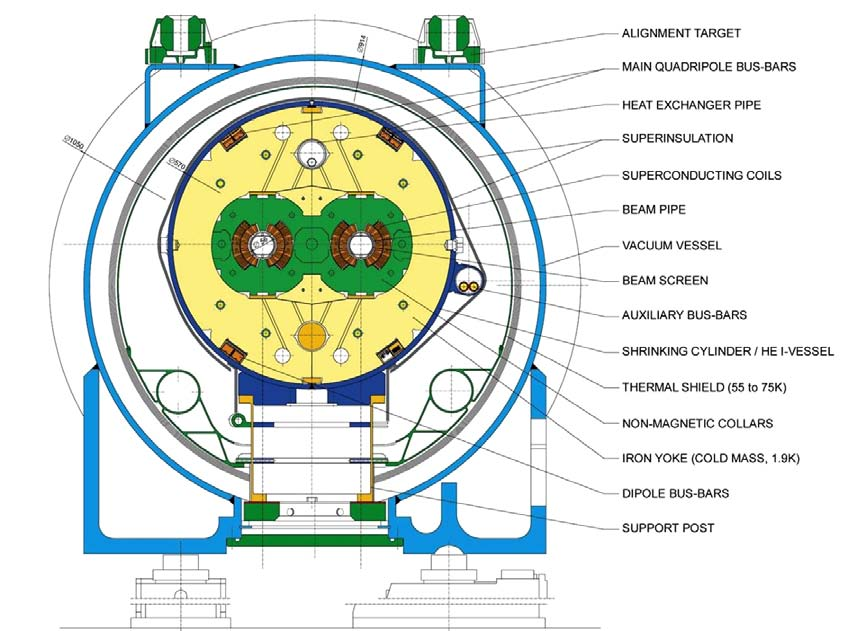
\includegraphics[width=0.8\textwidth]{experiment/lhcDipole.png}
  \caption[LHC dipole schematic]{
    Schematic cross section of an LHC dipole and its attendent electrical and cryogenic infrastructure, reproduced from Ref.~\cite{Evans:2008zzb}.
    }\label{fig:lhcDipole}
\end{figure}

Because no single accelerator has the dynamic range necessary to take a stationary proton to \TeV-scale energies, a chain of smaller accelerators repurposed from previous experiments feeds moderate-energy protons into LHC\@.
Protons are obtained by ionizing hydrogen atoms, then accelerated to $50\MeV$ by the Linac~2 linear accelerator and injected into the Proton Syncrotron Booster~(PSB), the first of several circular accelerators.
The PSB feeds $1.4\GeV$ protons into the Proton Synchrotron~(PS), which in turn injects them into the Super Proton Synchrotron~(SPS) at $26\GeV$.
The protons are then accelerated to $450\GeV$ in the SPS before being injected into LHC\@.
A diagram of the entire accelerator chain is shown in Fig.~\ref{fig:acceleratorChain}.

\begin{figure}[htbp]
  \centering
  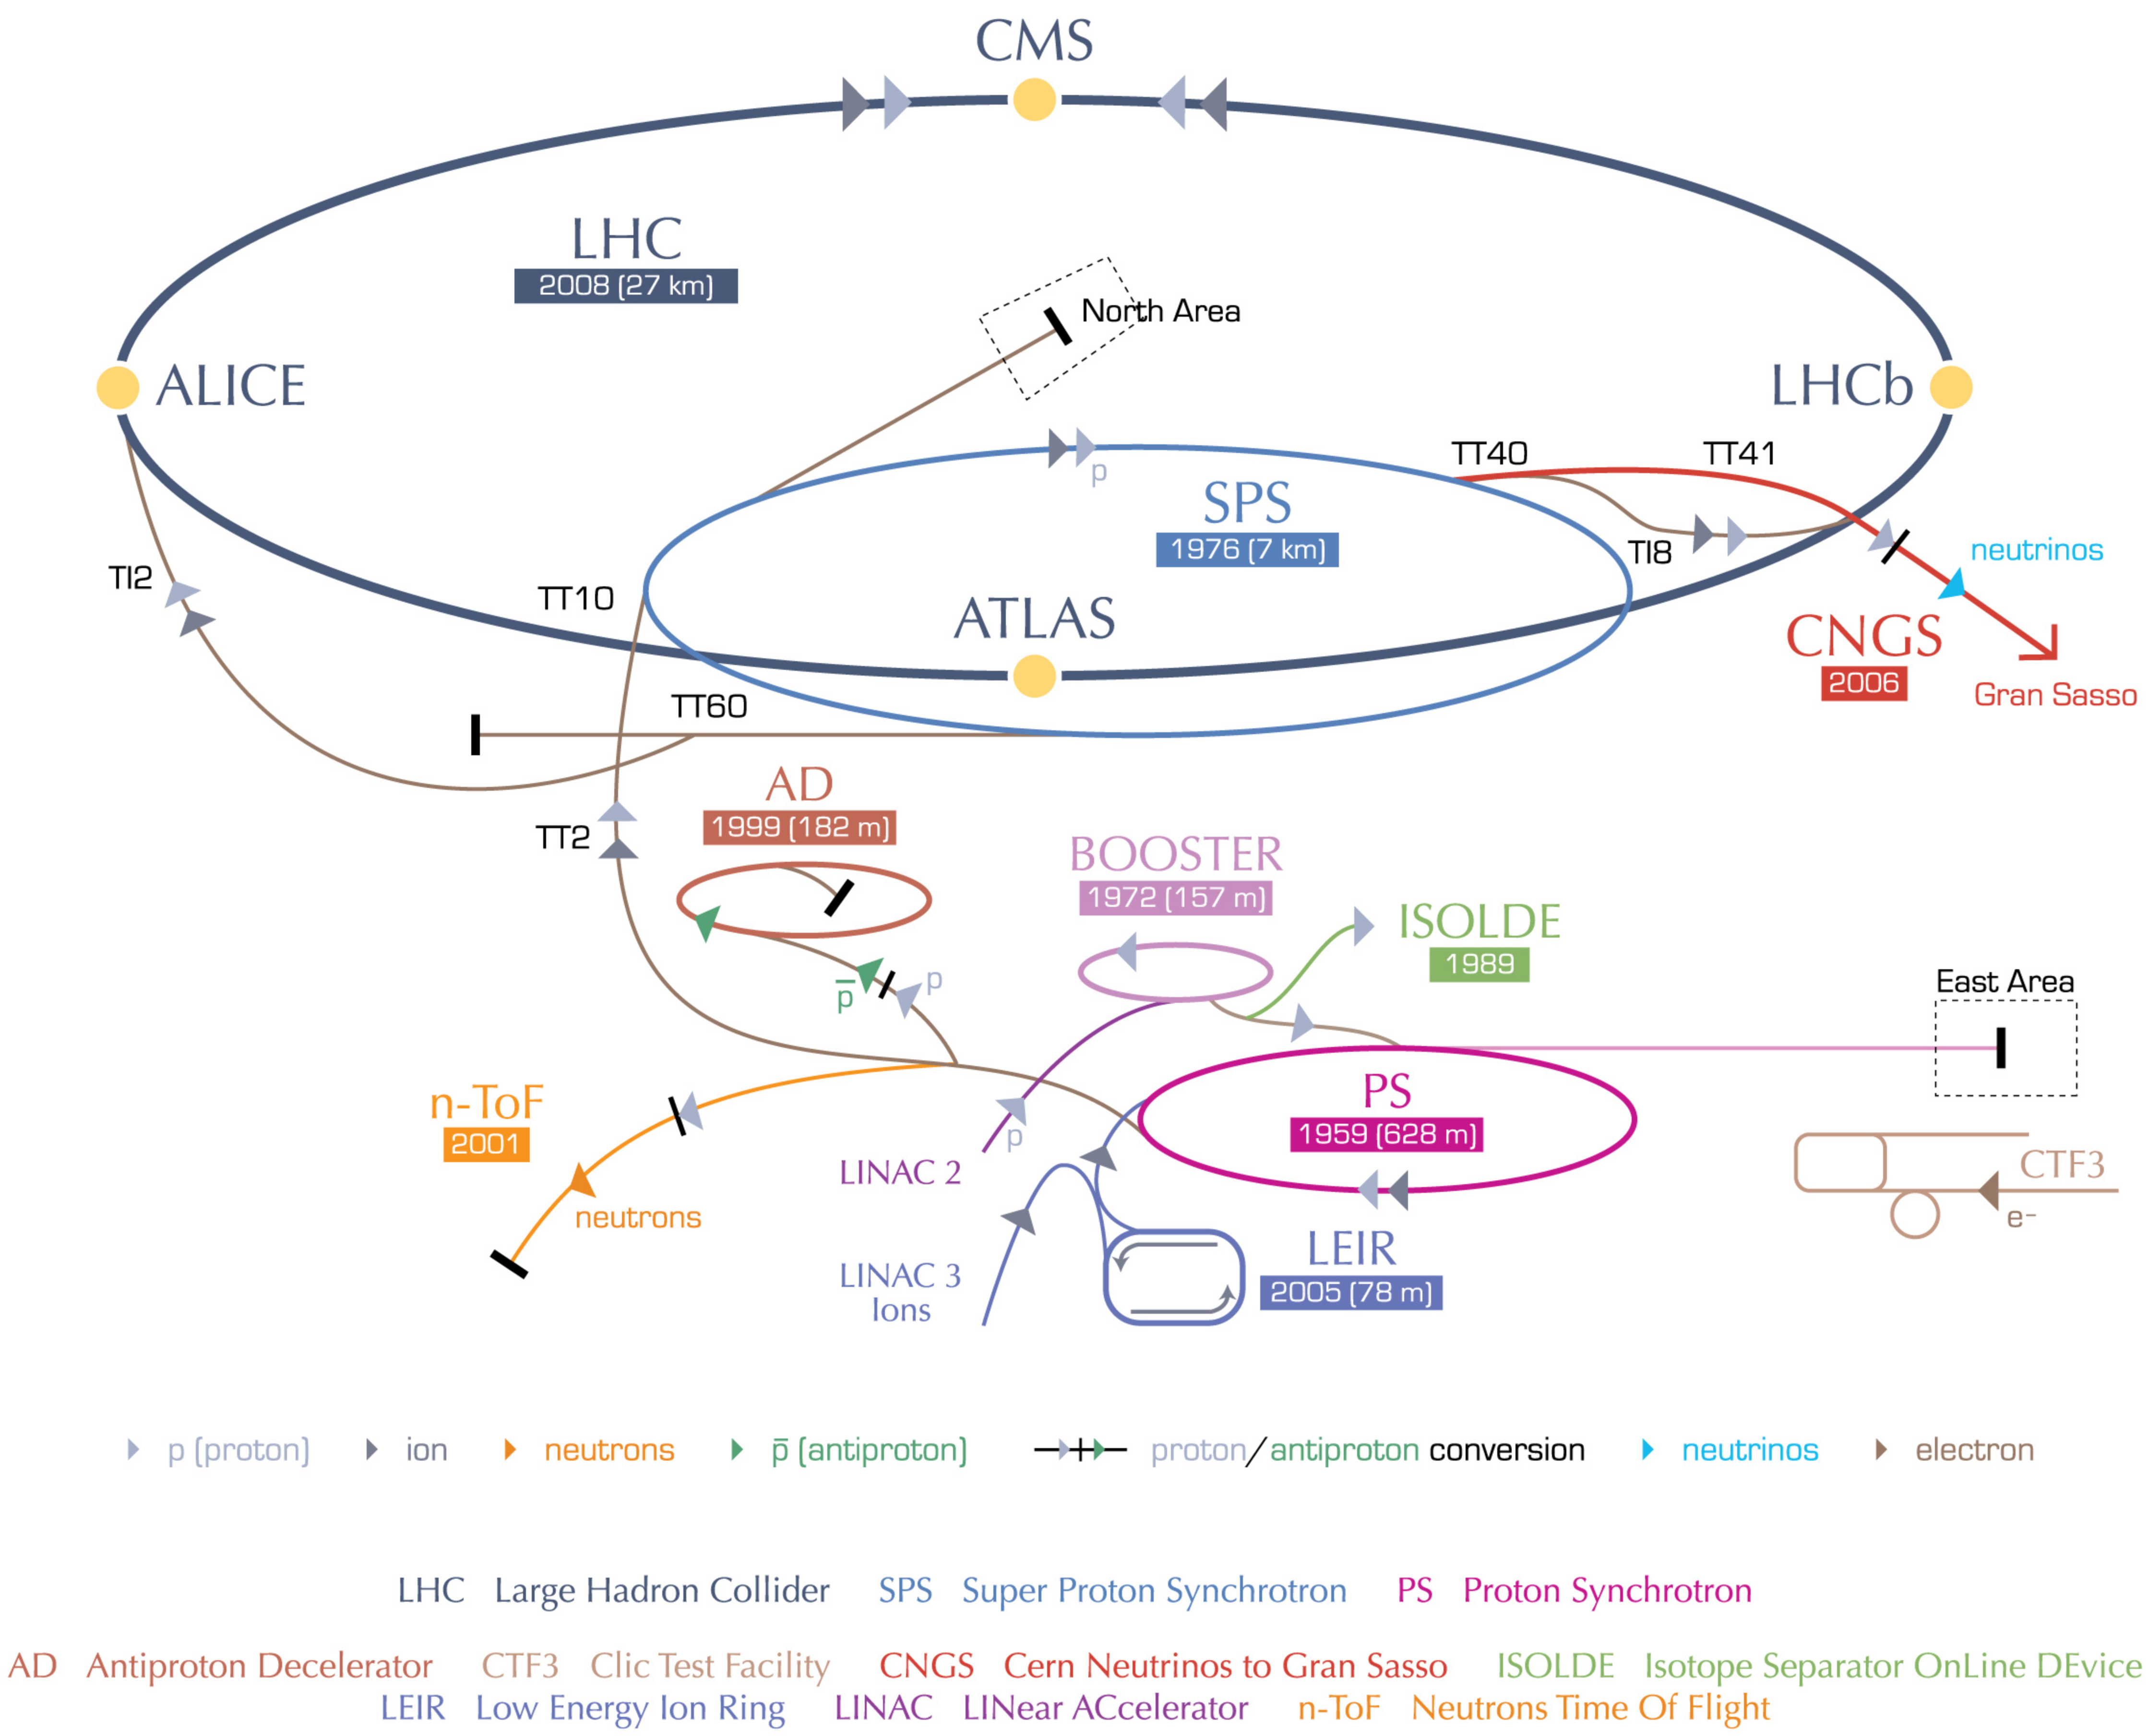
\includegraphics[width=\textwidth]{experiment/acceleratorChain.png}
  \caption[LHC accelerator and experiment layout]{
    A schematic of the LHC accelerator chain and peripheral experiments, reproduced from Ref.~\cite{Christiane:1260465}.
  }\label{fig:acceleratorChain}
\end{figure}

The LHC ring is divided into eight sectors, each of which features a $528\unit{m}$ straight section connected to the adjacent sections by $2.45\unit{km}$ arcs.
The straight section length was set by the need for RF cavities to accelerate LEP beams to counteract synchrotron radiation, which is a primary factor limiting electron and positron beam energy.
This is not ideal for proton beams; protons' much higher mass means they radiate less and need fewer RF cavities.
The straight sections feature access points numbered with Point~1 at the main CERN site in Meyrin, Switzerland, and the rest numbered~2--8, increasing in the clockwise direction when viewed from above.
Points~1, 2, 5, and~8 have beam crossing points and host detectors to study the resulting proton-proton collisions.
Points~3 and~7 feature collimators to reduce momentum and betatron nonuniformities in the beams.
The RF cavities are at Point~4 and the beams are dumped after use or in the event of a magnet quench at Point 6\@.
Beams are disbursed and deflected into an 8\unit{m} long water-cooled graphite absorber by fast kicker magnets which activate in a 3\unit{\mu{} s}-long bunch-free region of the beam known as the abort gap.

The CMS detector is at Point~5 in Cessy, France, the furthest point on the ring from the Meyrin site and Point~1, which houses ATLAS~\cite{Aad:2008zzm}, a similar but fully independent general-purpose particle detector.
CMS and ATLAS use complementary detector technology so that any measurement or discovery by one can be made concurrently or verified by the other.
The other two experimental insertions feature specialized detectors studying collisions at lower-luminosity beam interaction points.
The LHCb detector~\cite{Alves:2008zz}, at Point~8, studies hadronic physics with an emphasis on b-hadrons, and ALICE~\cite{Aamodt:2008zz} studies heavy ion collisions at Point~2\@.
Three smaller experiments share interaction points with the larger detectors, with TOTEM~\cite{Anelli:2008zza} studying proton structure and the total proton-proton interaction cross section next to CMS\@; LHCf~\cite{Adriani:2008zz} studying the $\pi^0$ energy spectrum and multiplicity near ATLAS\@; and MoEDAL~\cite{Acharya:2014nyr} searching for magnetic monopoles or other heavy, stable, ionizing particles at Point~8 with LHCb.



\subsection{Operating Parameters}
With the beam energy set by the radius of the ring and the strength of available magnets, the number of interesting physics events produced in LHC collisions depends only on the integrated luminosity
\begin{equation}
  \lumiL_\textit{int} = \int \lumiL \cmsSymbolFace{d}t,
\end{equation}
where $\lumiL$ is the instantaneous luminosity defined in Eq.~\ref{eq:instLumi} and the integral runs over the time the machine spends in collisions mode.
LHC's availability for collisions depends on the electrical and mechanical stability of the accelerators and their support systems, including the cryogenics and the vacuum in the beam pipe.
The instantaneous luminosity while running depends only on the beam parameters.
For symmetric beams which each have $n_b$ colliding gaussian bunches of intensity (i.e.\ number of protons in the bunch) $N_b$, orbiting the ring with frequency $f_\textit{rev}$ and relativistic factor $\gamma=E_p/m_p$, the instantaneous luminosity is give by
\begin{equation}
  \lumiL = f_\textit{rev} \frac{n_b N_b^2 \gamma}{4\pi \beta^\ast \epsilon_N} R,
\end{equation}
where $\beta^\ast$ is the amplitude of the beams' betatron oscillations around the nominal ring path at the interaction point, the normalized emittance $\epsilon_N$ is a measure of the beams' spread in both position and momentum space, and $R$ is a geometrical factor accounting for the beam crossing angle,
\begin{equation}
  R = \sqrt{1 + \left(\frac{\theta_c \sigma_z}{2\sigma^\ast}\right)^2}.
\end{equation}
Here $\theta_c$ is the beams' crossing angle, and $\sigma_z$ and $\sigma^\ast$ are respectively the longitudinal and transverse RMS widths of the bunches in the lab frame.


\subsubsection{Design}
The machine parameters in the LHC design specification can be seen in the first column of Table~\ref{tab:lhcparams}.
Machine parameters during data taking have in general been quite different, due to both technological advances and technical challenges.
In particular, beam energy and number of colliding bunches are both lower than designed due to commissioning issues with the magnets and their safety systems~\cite{Bajko:1168025}, but increases in the number of collisions per bunch crossing (``pileup'') have more than compensated, leading to a peak instantaneous luminosity in 2016 that was more than 50\% higher than designed.
Operating parameters have changed frequently during data taking and upgrades are always ongoing.


\begin{table}
\caption[LHC beam parameters]{
  LHC beam parameters as designed and in practice.
  As stated in the text, $n_b$ is the number of colliding bunches, $N_b$ is the number of protons in each bunch, $\beta^\ast$ is the betatron amplitude at the interaction point, $\epsilon_N$ is the normalized emittance, and $\lumiL_{\left(\textit{int}\right)}$ is the instantaneous (integrated) luminosity.
  }
\centering
\begin{tabular}{lllllll}
\toprule
                                                                     & \multicolumn{1}{c}{Design} & \multicolumn{3}{c}{Run I}  & \multicolumn{2}{c}{Run II} \\
\midrule
Year                                                                 &          & 2010    & 2011    & 2012    & 2015    & 2016                               \\
\midrule\midrule
Energy per beam $\left(\TeVns\right)$                                & 7        & 3.5     & 3.5     & 4       & 6.5     & 6.5                                \\
Bunch spacing $\left(\unitns{ns}\right)$                             & 25       & 150     & 50      & 50      & 25      & 25                                 \\
$n_b$                                                                & 2808     & 348     & 1331    & 1368    & 2232    & 2208                               \\
$N_b \left(10^{11}\right)$                                           & 1.15     & 1.2     & 1.5     & 1.7     & 1.15    & 1.25                               \\
$\beta^\ast \left(\unitns{m}\right)$                                 & 0.55     & 3.5     & 1.0     & 0.6     & 0.8     & 0.4                                \\
$\epsilon_N \left(\unitns{mm}\unit{mrad}\right)$                     & 3.75     & 2.2     & 2.3     & 2.5     & 3.5     & 3.0                                \\
Peak pileup                                                          & FIXME    & 4       & 17      & 37      & 22      & 49                                 \\
Peak $\lumiL \left(10^{34}\unitns{cm}^{-2}\unitns{s}^{-1}\right)$    & 1        & 0.02    & 0.35    & 0.77    & 0.52    & 1.53                               \\
$\lumiL_\textit{int} \left(\fbinvns\right)$                          &          & 0.04    & 6.1     & 23.3    & 4.2     & 41.1                               \\
\bottomrule

\end{tabular}\label{tab:lhcparams}
\end{table}


\subsubsection{Run I}
The LHC came online in 2010 with a beam energy of $3.5\TeV$, which was increased to $4\TeV$ in 2012.
Bunches were spaced $50\unit{ns}$ apart instead of $25\unit{ns}$ to allow full exploitation of excellent injection chain performance~\cite{1742-6596-455-1-012001}.
Beams exiting the SPS had bunch intensity as much as 50\% higher than anticipated in the original LHC design and beam emittance as low as 67\% of nominal.
This allowed the LHC to achieve 77\% of its design instantaneous luminosity in 2012 despite having roughly half as many bunches in each beam.

Machine availability was overall good considering the complexity and relative newness of the LHC, with about 36\% of scheduled time spent in stable beams.
In all, LHC delivered $6.1\fbinv$ to CMS and ATLAS in 2011 and $23.3\fbinv$ in 2012, enough to allow discovery of the Higgs boson.
The integrated luminosity for each year of LHC operation is shown as a function of calendar month and day in Fig.~\ref{fig:intLumi}.

\begin{figure}[htbp]
  \centering
  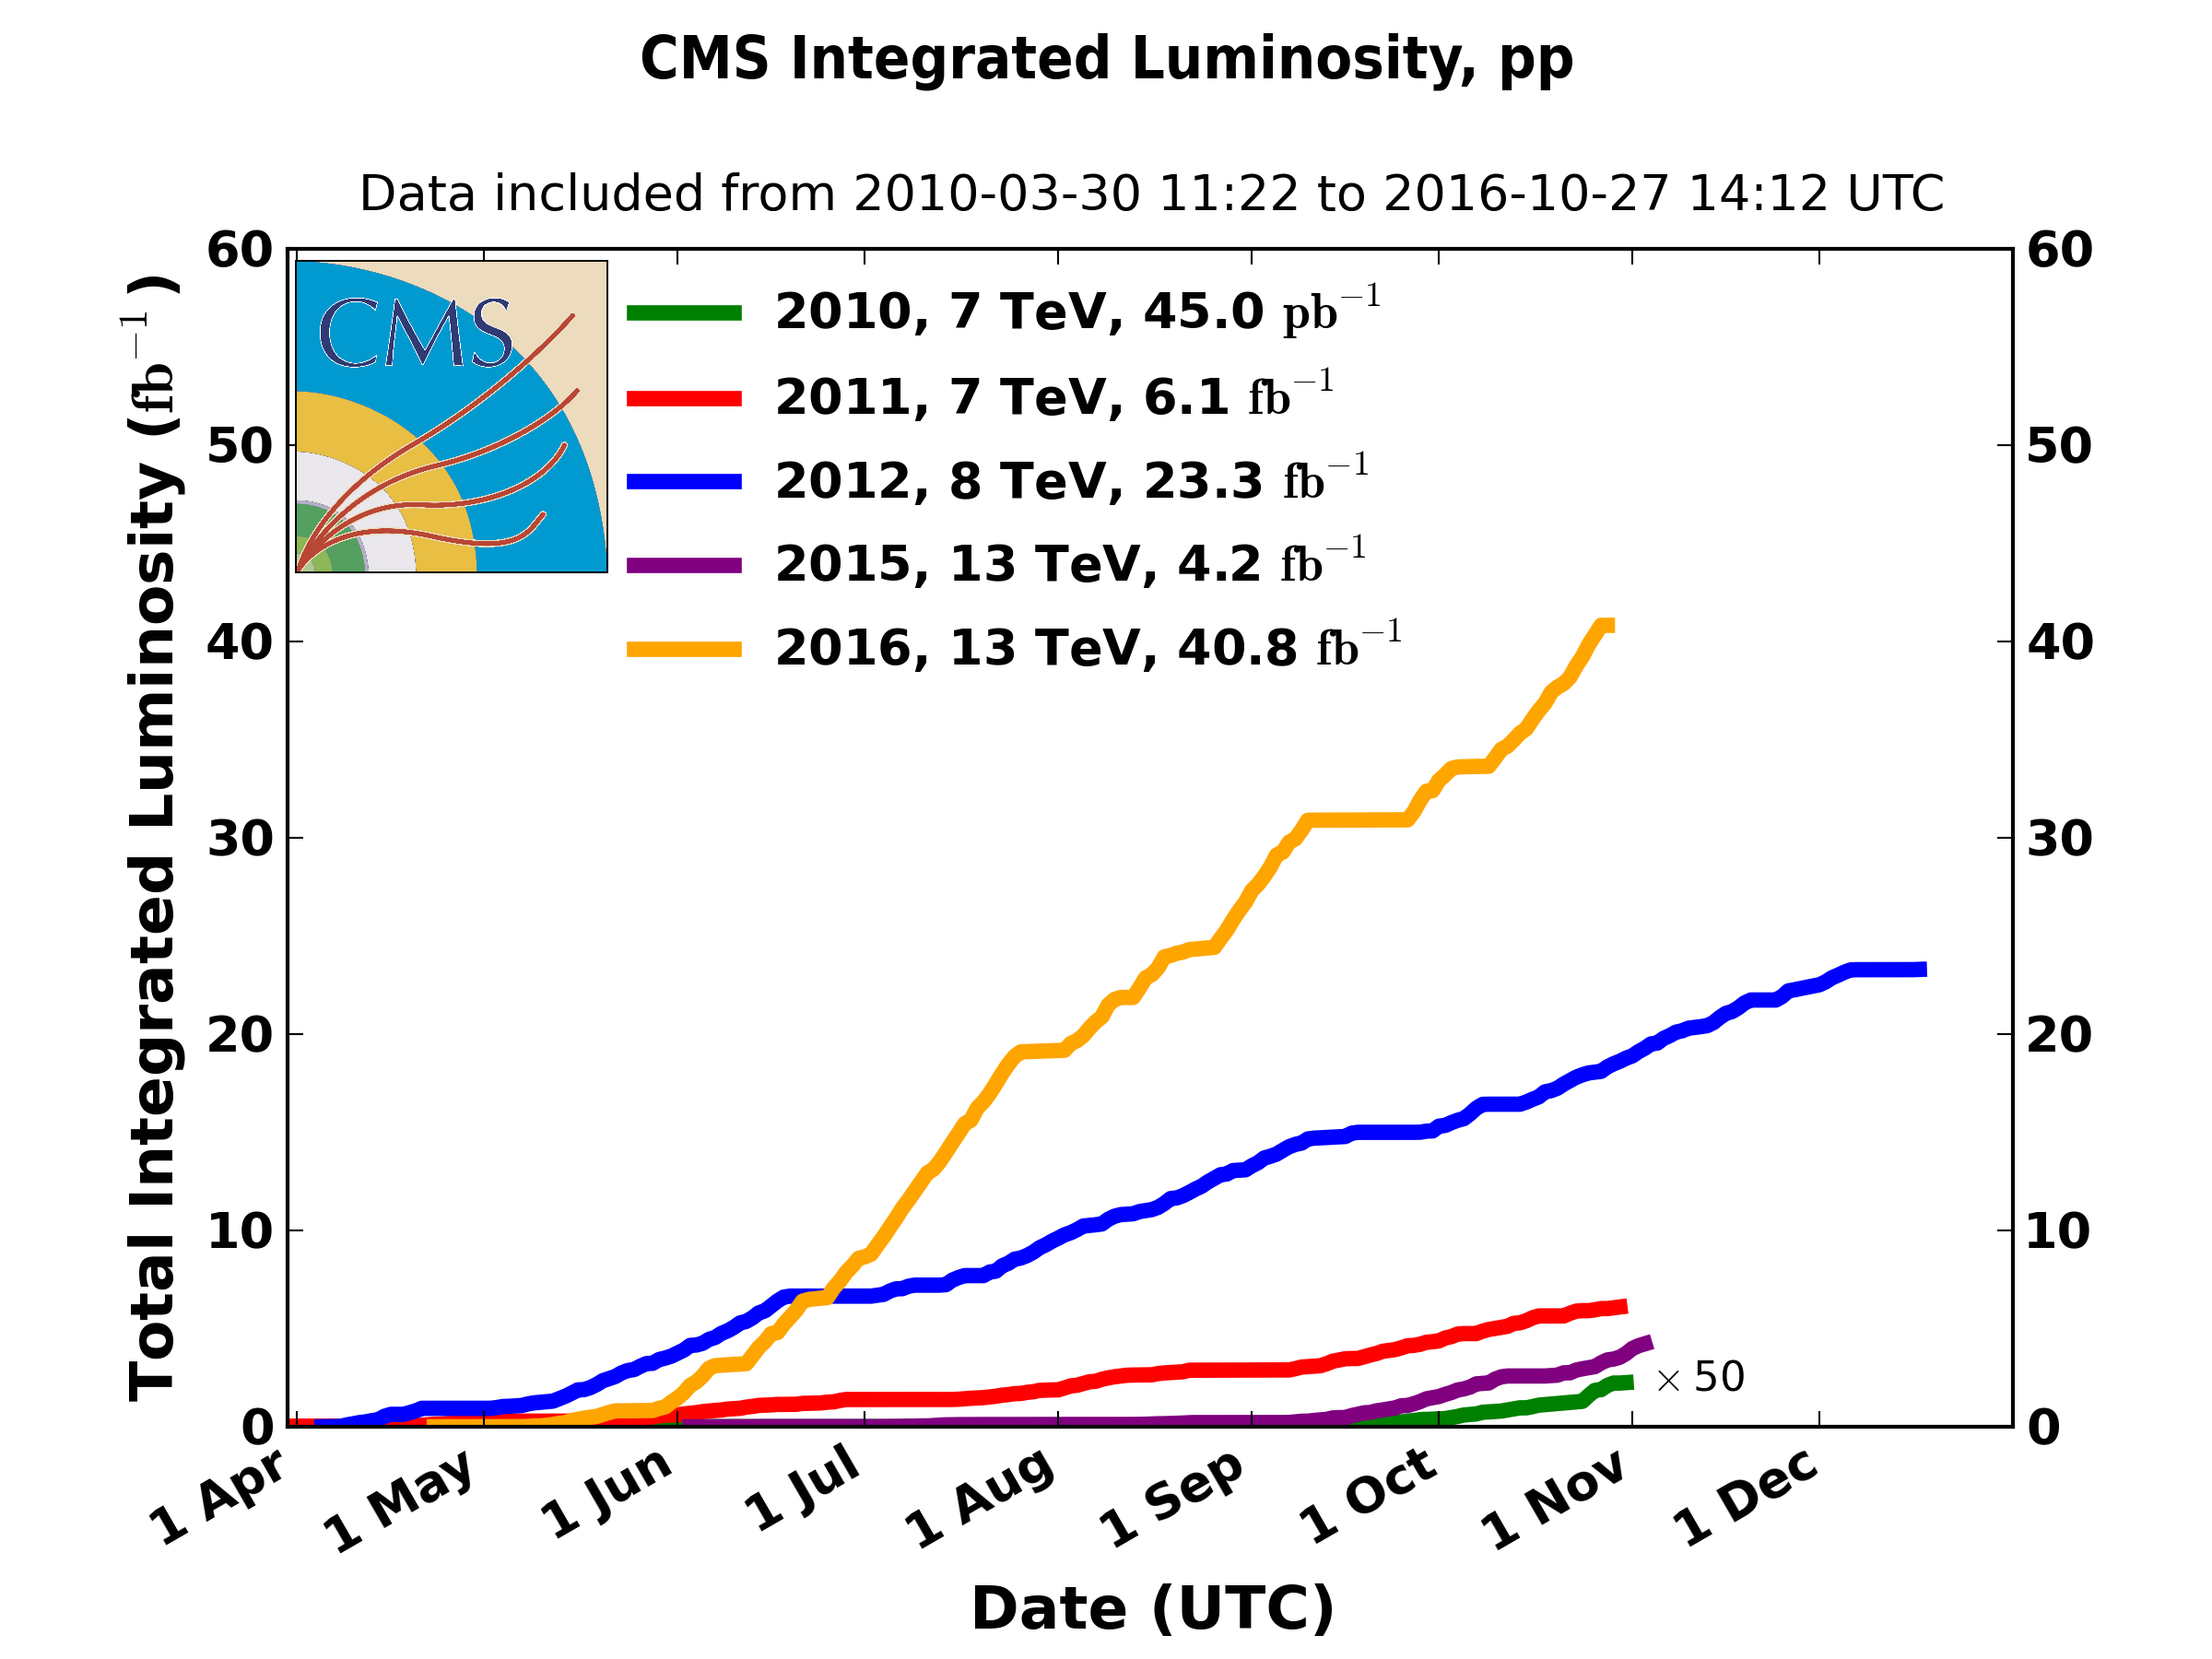
\includegraphics[width=.7\textwidth]{experiment/intLumi.png}
  \caption[Integrated luminosity delivered to CMS in each LHC run period]{
    The integrated luminosity delivered to CMS in each year of LHC operation, shown as a function of the date within the year.
  }\label{fig:intLumi}
\end{figure}


\subsubsection{Run II}
The LHC shut down for 2013 and 2014 to allow a number of repairs and upgrades, including measurements, repairs and upgrades on the electrical connections and cryogenic safety systems.
Beam energies were increased to $6.5\TeV$, close to the nominal $7\TeV$.
The bunch spacing was decreased to $25\unit{ns}$ while maintaining low emittance and high bunch intensity with the implementation of the beam compression merging and splitting (BCMS) scheme in which bunches are merged in the PS before they are split for injection into SPS, allowing higher bunch intensity~\cite{Papaphilippou:2014qwa}.
This was offset by vacuum problems in the SPS beam dump, which limited the total number of colliding bunches to around 2200~\cite{Frederick:2235979}.
Improvements in collimators and beam optics reduced $\beta^\ast$ to $40\unit{cm}$ in 2016, lower than the design $\beta^\ast$ of $55\unit{cm}$.
Overall instantaneous luminosities were substantially higher than originally designed.

Machine availability in Run II was excellent, with over 60\% of planned time spent in stable beams~\cite{Frederick:2235979}.
The world's first $13\TeV$ collisions in 2015 were the subject of a number of measurements and searches, though the $4.2\fbinv$ integrated luminosity delivered to Points~1 and~5 in 2015 was less than planned due to several mechanical issues.
The integrated luminosity acheived in 2016, $41.1\fbinv$, was far above the roughly $25\fbinv$ expected and more than all previous runs combined, allowing measurements and searches of unprecedented sensitivity and reach, including those presented in this Thesis.



%-------------------------------------------------------------------------------
% CMS
%-------------------------------------------------------------------------------

\section{The Compact Muon Solenoid Detector}
The CMS detector~\cite{Chatrchyan:2008zzk} is a general-purpose particle detector located in a cavern roughly $100\unit{m}$ below the surface at LHC Point~5.
Though designed to do a wide range of physics analyses, CMS was designed specifically with Higgs boson discovery in mind.
Primary design goals include
\begin{itemize}
  \item High-efficiency reconstruction of charged particles with precise measurement of their trajectories and momenta
  \item Good electromagnetic energy resolution, including diphoton and dielectron mass resolution
  \item Hermetic calorimetry for good missing transverse energy and dijet mass resolution
  \item Good muon identification, momentum resolution (including dimuon mass resolution), and charge determination over a broad range of energies
\end{itemize}
To this end, CMS features a silicon tracker, a scintillating crystal electromagnetic calorimeter (ECAL), and a hermetic hadronic calorimeter (HCAL) inside a $3.8\unit{T}$ solenoid magnet surrounded by ionized gas muon tracking devices, all of which can be seen as part of the whole detector in Fig.~\ref{fig:cmsWhole}.
Decisions on which events to read out are made on-line by a two-level trigger system.
Descriptions of these systems follow.

\begin{figure}[htbp]
  \centering
  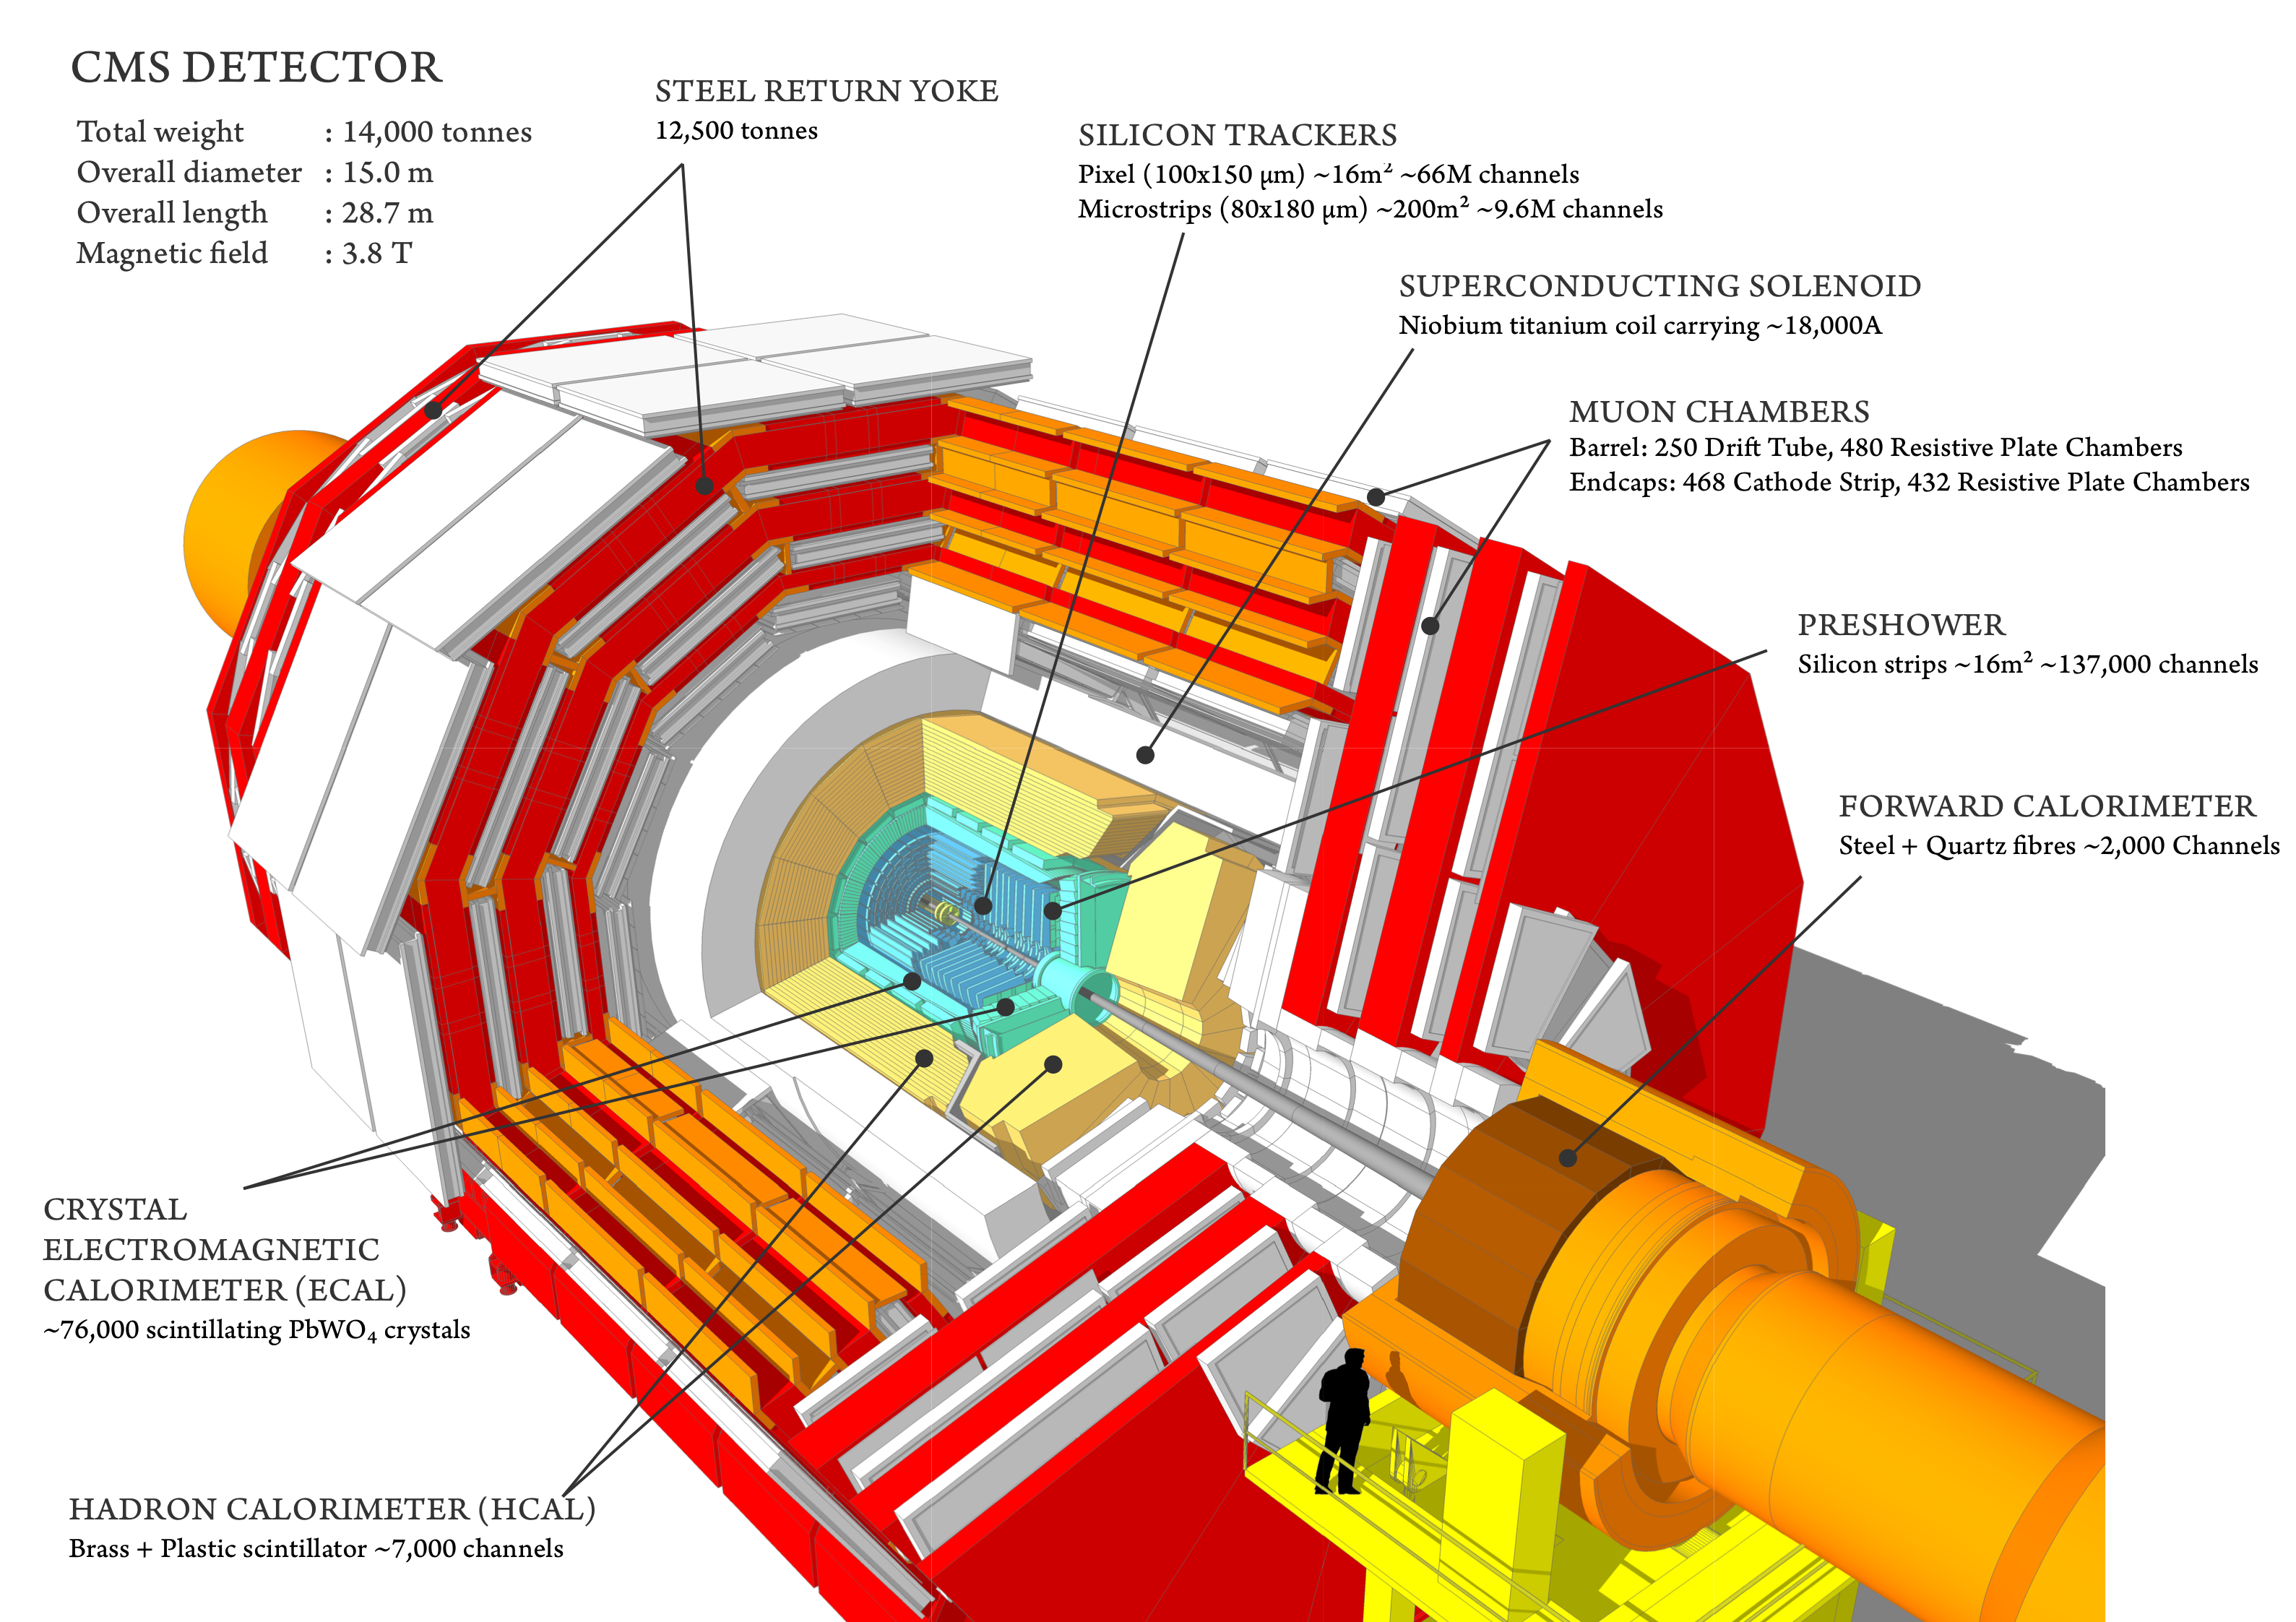
\includegraphics[width=\textwidth]{experiment/cmsWhole.png}
  \caption[CMS cutout schematic]{
    Cutout schematic of CMS with all major subdetectors, the beamline, the magnet, and the return yoke visible. Reproduced from Ref.~\cite{Sakuma:1626816}.
  }\label{fig:cmsWhole}
\end{figure}

\subsection{Terminology and Geometry}
The CMS detector systems are arranged in cylindrical layers with the interaction point at the center, serving as the origin for the coordinate system.
The coordinate system is defined with the positive-$x$ direction pointing toward the center of the ring, positive-$y$ pointing vertically up, and positive-$z$ pointing parallel to the beam in the counterclockise direction when the LHC ring is viewed from above.
Particle momenta are typically expressed in quasicylindrical coordinates $\left(\pt,\eta,\phi\right)$.
Here $\pt$ is the magnitude of the particle's momentum transverse to the beam
\begin{equation}
  \pt \equiv \sqrt{p_x^2 + p_y^2},
\end{equation}
and $\phi$ is the azimuthal angle, i.e.\ the angle from the $x$-axis to the particle's trajectory in the $x$-$y$ plane.
The pseudorapidity~$\eta$ is defined as
\begin{equation}
  \eta \equiv -\ln \left[\tan\left(\frac{\theta}{2}\right)\right]
\end{equation}
where $\theta$ is the polar angle measured from the $z$-axis.
The relativistic rapidity
\begin{equation}
  y \equiv \frac{1}{2} \ln \left(\frac{E+p_z}{E-p_z}\right),
\end{equation}
converges to the pseudorapidity in the limit of massless particles.
Pseudorapidity is preferred to rapidity because it is purely geometrical, with no dependence on the particle energy.
Both are preferred over $\theta$ because rapidity differences are invariant under longitudinal boosts, and because hadron flux at colliders is roughly constant as a function of rapidity.
The transverse energy~$\et$ is the the magnitude of the particle's four-momentum transverse to the beam, equal to $\pt$ in the limit of massless particles.
Spatial coordinates are expressed as $\left(r,\eta,\phi\right)$, where $r$ is the distance from the beam in the $x$-$y$ plane.


\subsection{Magnet and Inner Tracking System}
A particle of charge $q$ moving through a uniform magnetic field of strength $B$ that points in the $z$ direction will travel in a helix of radius $R$, given by
\begin{equation}
  R = \frac{\pt}{\lvert q\rvert B},
\end{equation}
with the chirality of the helix determined by the sign of $q$.
Thus one can determine the transverse momentum of the particle by measuring its path through the magnetic field and finding the radius of curvature.
In practice, all but the lowest-energy particles leave too short an arc in the detector for direct measurement of the radius, so the sagitta of the arc is used instead, given by
\begin{equation}
  s = \frac{qBL^2}{8\pt}
\end{equation}
where $L$ is the length of the chord spanning the arc (typically equal to the radius of the tracking system).
The transverse momentum resolution varies as
\begin{equation}
  \frac{\delta \pt}{\pt} \propto \frac{\pt}{BL^2},
\end{equation}
so a strong field and a large tracking volume are vital to keeping measurements precise even at high energies.

To this end, CMS contains the world's largest superconducting magnet\footnote{Largest in the sense of having the largest stored energy when at constant full field. The largest by size is the ATLAS barrel toroid.}, a solenoid $13\unit{m}$ long and $6\unit{m}$ in diameter, which generates a nearly-uniform $3.8\unit{T}$ field in the centralmost part of the detector~\cite{Campi:magnetTDR}.
To measure the paths of charged particles in the field, the volume closest to the interaction point contains layers of silicon sensors that detect hits from charged particles with high efficiency and excellent position resolution, between $4.4\unit{cm}$ and $1.1\unit{m}$ from the beam for $2.7\unit{m}$ on either side of the interaction point.
This system, called the inner tracker and shown schematically in Fig.~\ref{fig:tracker}, consists of an inner pixel detector surrounded by a larger silicon strip detector.
Both consist of concentric cylinders of sensors covering the barrel of the detector capped by discs covering the high-$\eta$ region, up to $\abseta < 2.5$.
With a total of roughly $200\unit{m}^2$ of silicon, the inner tracker is the largest silicon tracker in the world.
Tracks may be reconstructed with hits in as many as 14 layers.
The downside of this is that the tracker and its mechanical support structure represent a substantial amount of material for electrons and photons to interact with before they reach the calorimeters, with total material budget between 0.4 radiation lengths ($\eta=0$) and 1.8 radiation lengths ($\abseta \approx 1.4$), as shown in Fig.~\ref{fig:trackerMaterial}.
The tracker-only $\pt$ uncertainty is around~1.2\% at $200\GeV$ and 15\% at~$1\TeV$.
Tracker readout is too slow for it to be used in the L1 trigger (see Section~\ref{sec:l1trig}), the first set of trigger decisions must be made using only information from the calorimeters and outer muon system.

\begin{figure}[htbp]
  \centering
  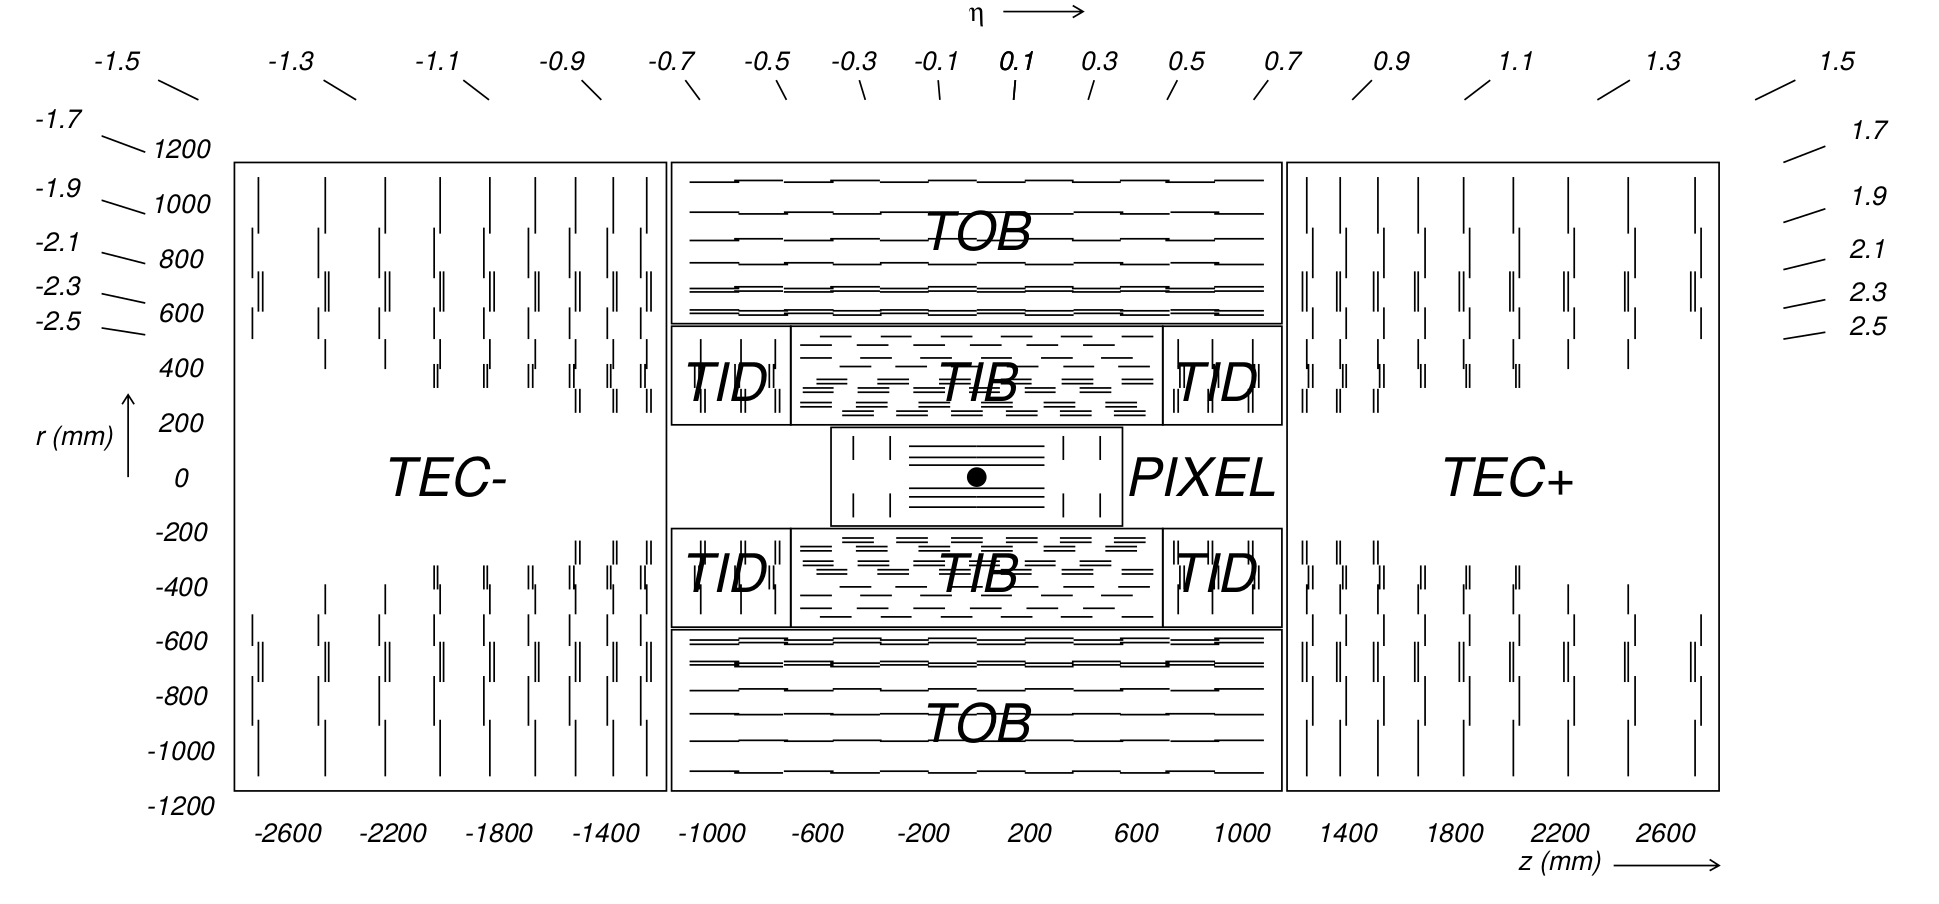
\includegraphics[width=\textwidth]{experiment/tracker.png}
  \caption[Inner tracker layout]{
    Diagram of the inner tracker layout, reproduced from Ref.~\cite{Chatrchyan:2008zzk}.
  }\label{fig:tracker}
\end{figure}


\begin{figure}[htbp]
  \centering
  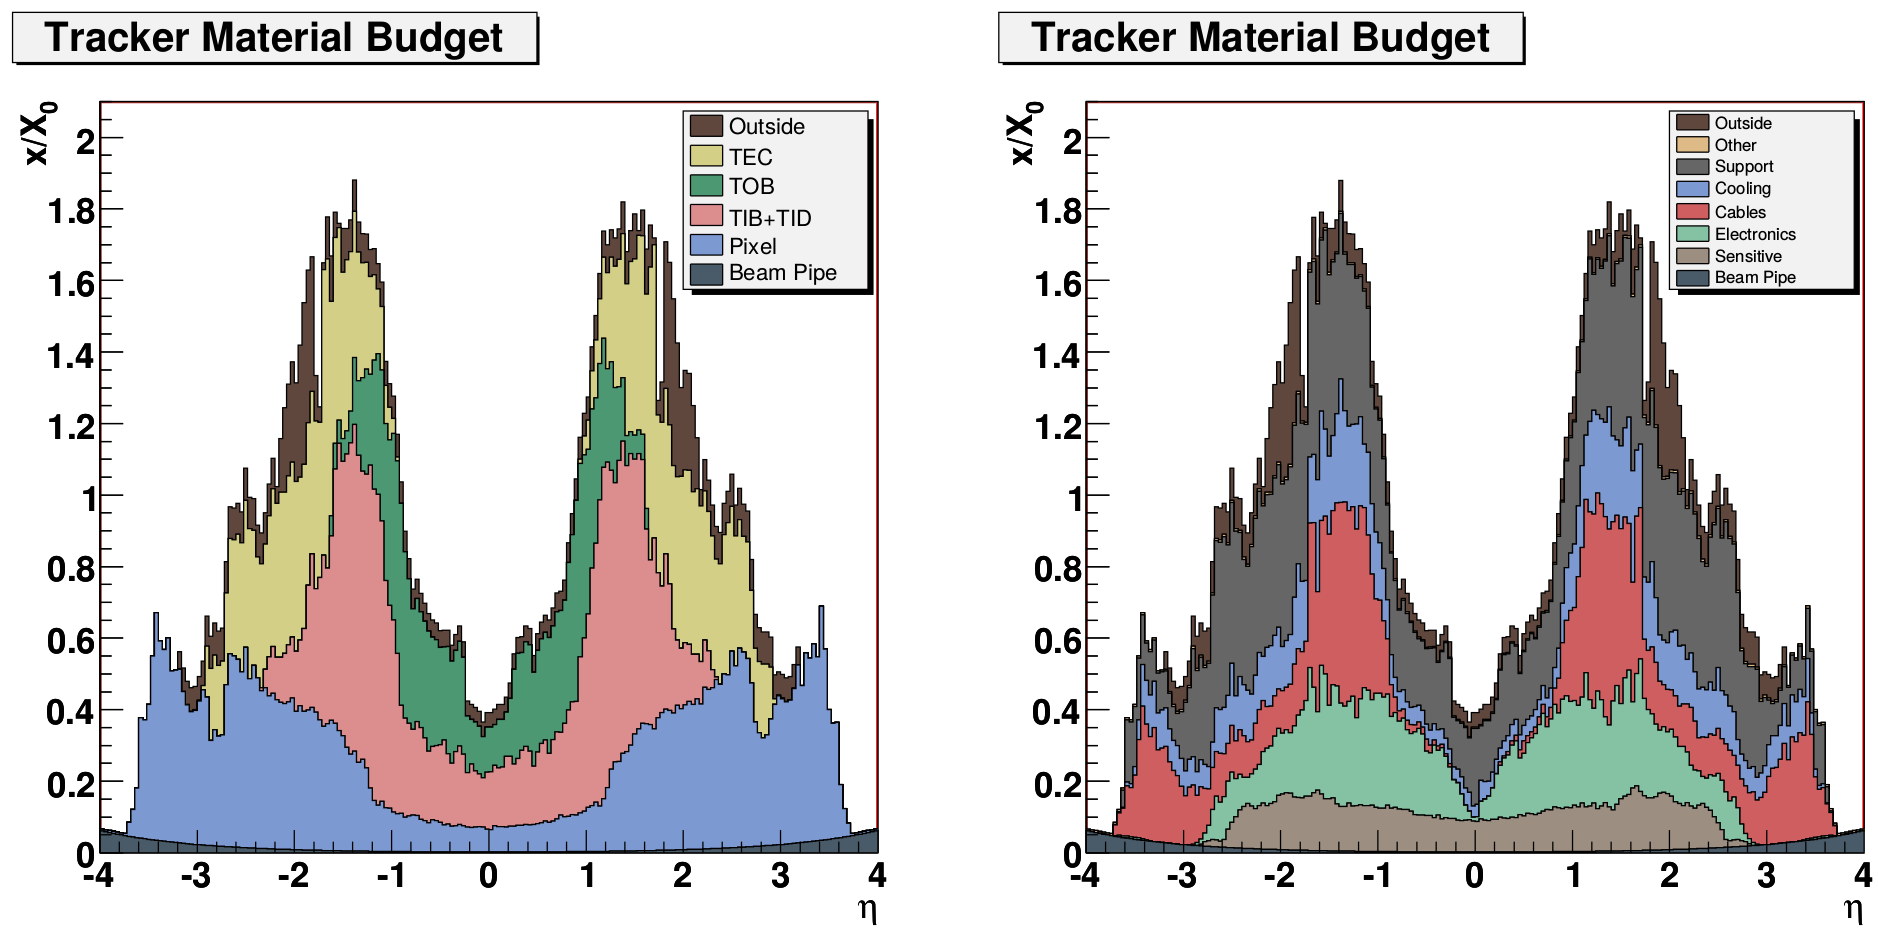
\includegraphics[width=\textwidth]{experiment/trackerMaterial.png}
  \caption[Tracker material budget in radiation lengths]{
    Total tracker material budget in units of electromagnetic radiation lengths, as a function of pseudorapidity.
    At (left) the total is divided by detector subsystem, at (right) by the function of the material. Reproduced from Ref.~\cite{Chatrchyan:2008zzk}.
  }\label{fig:trackerMaterial}
\end{figure}

As the system closest to the interaction point, the inner tracker is subject to extremely high radiation doses, equivalent to 840\unit{kGy} for the innermost pixel layer over an integrated luminosity of 500\fbinv, so radiation tolerance is a major design constraint for both the sensors and readout electronics~\cite{Karimaki:368412}.
Leakage currents in the sensors, which degrade sensor performace, increase linearly with radiation fluence and exponentially with temperature.
Because leakage currents cause self-heating in the silicon, they can create a dangerous positive thermal feedback loop if the sensors are not cooled below $-10\degree\unit{C}$ during operation.
Reverse annealing, a process by which radiation-induced defects in the silicon can cause further damage months after the radiation dose is received, can be mitigated by keeping the sensors below $0\degree\unit{C}$ at all times except for brief maintenance periods~\cite{Chatrchyan:2008zzk}.
Therefore, to improve tracker performance and increase the detectors' lifetimes, a gas cooling system is used to keep the strip tracker around $-15\degree\unit{C}$ and the pixel detector around $-20\degree\unit{C}$ during operation.


\subsubsection{Pixel Detector}
The pixel detector~\cite{Karimaki:368412}, consisting of three layers in the barrel and two in the endcap, is responsible for accurate reconstruction of primary proton-proton interaction vertices and secondary vertices from decays of $\Pqb$-hadrons or other long-lived particles, as well as providing ``seed'' tracks that may be used in strip tracker reconstruction.
As the system closest to the interaction point, the pixel system experiences the highest charged-particle flux and therefore must have extremely fine granularity to differentiate between nearby particles.
The 66~million pixels in the system have a cell size of $100 \times 150\unit{\mu m}^2$.
Interpolation of the analog signals from the individual pixels allows a final spatial resolution of $15\unit{\mu m}$ in each direction.
The outermost barrel layer is $10.2\unit{cm}$ from the beam, and the second endcap disk is $46.5\unit{cm}$ from the interaction point.
The sensor modules are arranged such that at least three sensors cover the solid angle within the pixel detector's acceptance.




\subsubsection{Strip Tracker}
Outside the pixels is the silicon strip tracker~\cite{Karimaki:368412}, extending out to $1.1\unit{m}$ in the $r$ direction and $\pm 2.8\unit{m}$ in the $z$ direction.
The tracker is divided into inner and outer subdetectors, each of which has both barrel cylinders and endcap discs.
In total, there are ten layers in the barrel and nine in each of the endcaps.
The inner tracker uses $320\unit{\mu m}$-thick sensors with a typical strip cell size of $10\unit{cm} \times 80\unit{\mu m}$, leading to hit resolutions of 23--$35\unit{\mu m}$.
The outer tracker uses $500\unit{\mu m}$-thick sensors with typical strip sizes up to $25\unit{cm} \times 180\unit{\mu m}$, leading to hit resolutions of 35--$53\unit{\mu m}$.


\subsection{Electromagnetic Calorimeter}
Outside of the tracker is the electromagnetic calorimeter (ECAL), which is designed to absorb and measure the energy of electrons and photons.
ECAL is made of 68,524 radiation tolerant lead tungstate (\pbwo) crystals arranged in a cylindrical barrel (EB) covering $\abseta < 1.444$ and two endcap discs (EE) covering $1.566 < \abseta < 3.0$.
The geometry of the ECAL barrel and endcap can be seen in Fig.~\ref{fig:ecal}; the small gap between the barrel and endcap is necessary to accommodate cabling and support structures for the tracker.
\pbwo{} crystals scintillate blue-green light and are optically transparent, so the resulting light can be read out by avalanche photodiodes (APDs) in the barrel and vacuum phototriodes (VPTs) in the endcap.
ECAL's granularity is set by \pbwo's small {Moli\`ere} radius of~$2.2\unit{cm}$, which is also the size of the square front faces of the barrel crystals, which flare out to $2.6\unit{cm}$ at the back, giving them a truncated pyramid shape covering a roughy $0.0174 \times 0.174$ area of $\eta$-$\phi$ space.
The endcap crystals go from $2.86\unit{cm}$ squares at the front to $3.0\unit{cm}$ at the back.

\begin{figure}[htbp]
  \centering
  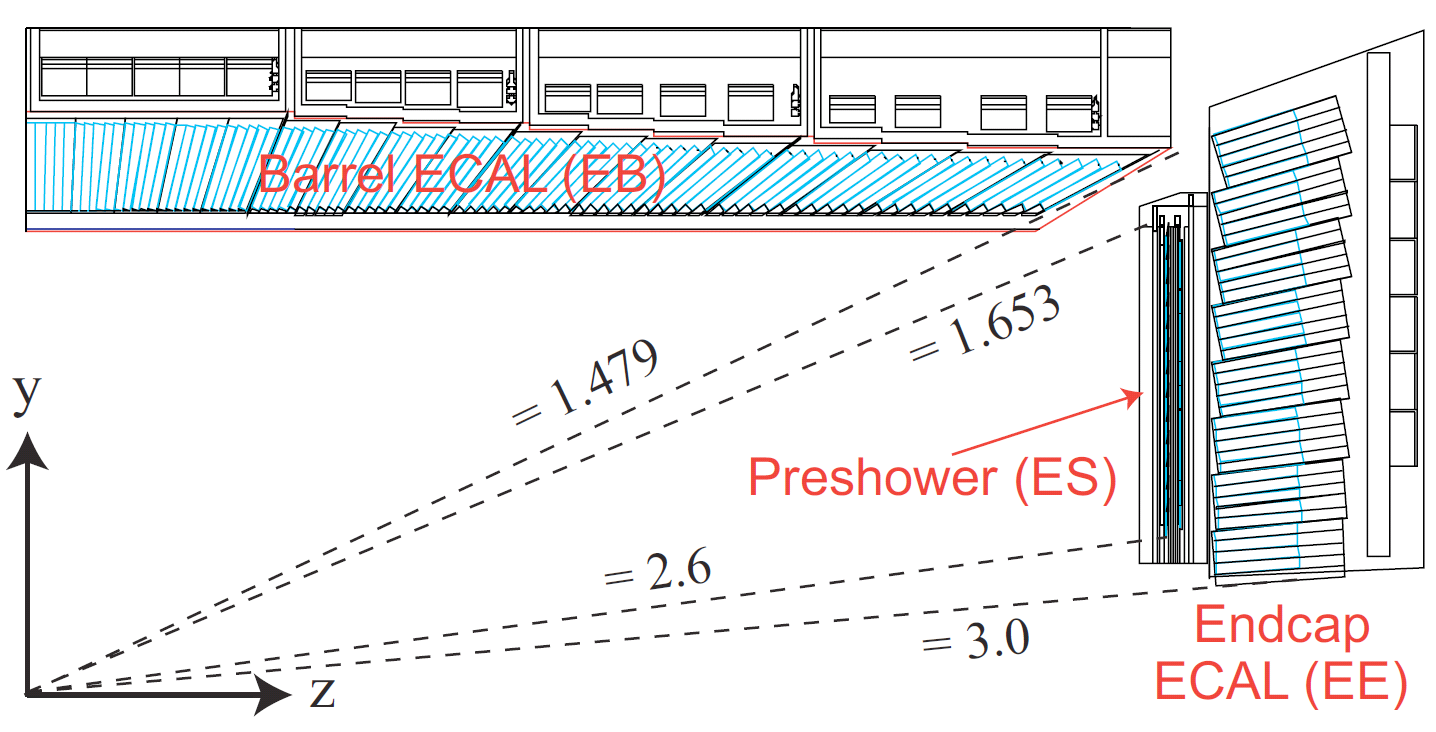
\includegraphics[width=0.7\textwidth]{experiment/ecal.png}
  \caption[ECAL geometry]{
    Diagram of ECAL geometry, reproduced from Ref.~\cite{Isildak:2013kfa}.
  }\label{fig:ecal}
\end{figure}

One of the primary design innovations of CMS---the eponymous compactness---was to place the calorimetry inside the magnet so that tracks can be unambiguously associated with energy deposits in the calorimeters without interference from scattering in the magnet coils.
This is possible in part thanks to the high density ($8.28\unit{g}/\unit{cm}^3$) and short radiation length ($0.89\unit{cm}$) of \pbwo, which allow ECAL crystals to be only $23\unit{cm}$ long in the barrel and $22\unit{cm}$ long in the endcap while still spanning 25.8 and 24.7 radiation lengths, respectively.
This is enough to ensure that few electrons or photons escape ECAL with any appreciable remaining energy.

The total scintillation light yield is relatively low, averaging just 4.5~photons per~$\MeVns$ deposited.
This is partially compensated by the fact that virtually all of ECAL is active material and no energy is lost to uninstrumented absorbers, but Poisson fluctuations in the yield are still the largest contribution to ECAL energy resolution for most electron and photon energies
This statistical uncertainty is represented by the first term in the full resolution equation,
\begin{equation}
  \left(\frac{\delta E}{E}\right)^2 = \left(\frac{2.8\%}{\sqrt{E/\GeVns}}\right)^2 + \left(\frac{0.12}{E/\GeVns}\right)^2 + \left(0.30\%\right)^2.
\end{equation}
The second term comes from electronic noise and noise from pileup, and the last term represents intrinsic differences between crystals.
The upside to \pbwo's scintillation is that it is fast: roughly 80\% of the light is emitted in the $25\unit{ns}$ between bunch crossings, so energy measurements require integration over only a few bunch crossings.


\subsection{Hadronic Calorimeter}
Between ECAL and the magnet is the hadronic calorimeter (HCAL), responsible for measuring the energy of hadronic jets.
HCAL is a sampling calorimeter, meaning that the hadrons pass through dense, uninstrumented material and the products of the resulting interactions deposit energy in scintillators which are used to measure the total energy of the original incoming particles.
The HCAL barrel (HB, $\abseta < 1.305$) and endcap (HE, $1.305 < \abseta < 3.0$) are made of layers of brass absorber interleaved with plastic scintillating tiles.
The energy resolution in HB and HE is given by
\begin{equation}
  \label{eq:HBHE_resolution}
  \left(\frac{\delta E}{E}\right)^2 = \left(\frac{90\%}{\sqrt{E/\GeVns}}\right)^2 + \left(4.5\%\right)^2.
\end{equation}
The first term is from the stochastic evolution of hadronic showers in the absorber, the second is from calibration uncertainties.

The geometry of HB, HE, and HO is shown in Fig.~\ref{fig:hcal}.
The thickness of HB and HE is constrained by the size of the magnet, varying from 5.4 nuclear interaction lengths in the central barrel to more than 10 in the endcaps.
Because HB is not thick enough to absorb all hadrons in the barrel, there is an extra outer HCAL component (HO) outside of the magnet, consisting of two more layers of scintillator on either side of a $20\unit{cm}$-thick iron ``tail catcher'' covering $\abseta < 1.3$.
With HO and the 1.1 interaction lengths in ECAL considered, no part of the calorimeter system spans fewer than 11.8 interaction lengths except in the gaps between barrel and endcap, minimizing the flux of hadronic ``punchthrough'' interacting with the muon system.
The total material budget in front of the layers of the muons systems is shown in Fig.~\ref{fig:hcalMaterial}.

\begin{figure}[htbp]
  \centering
  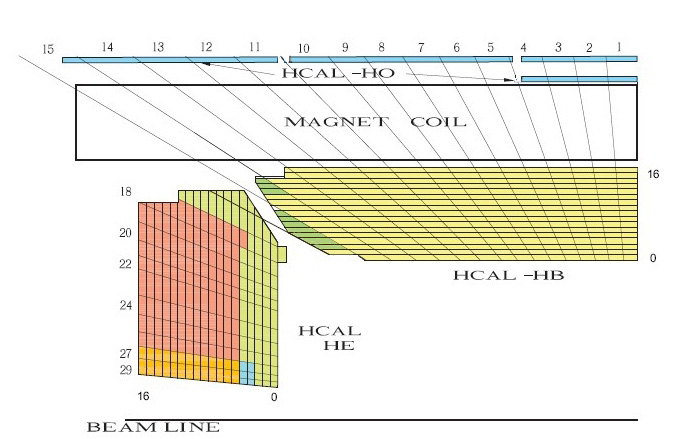
\includegraphics[width=\textwidth]{experiment/hcal.png}
  \caption[HCAL geometry]{
    Diagram of HCAL geometry, reproduced from Ref.~\cite{Chatrchyan:2008zzk}.
  }\label{fig:hcal}
\end{figure}

\begin{figure}[htbp]
  \centering
  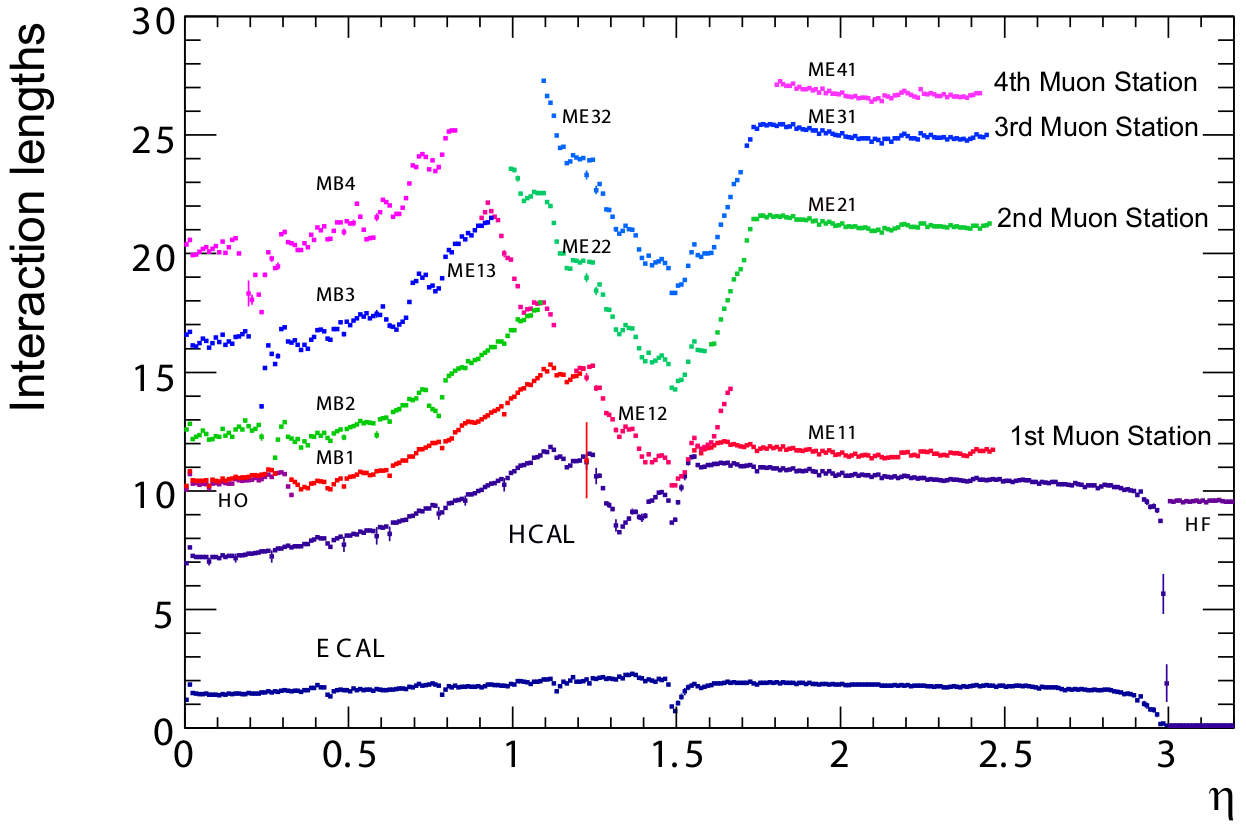
\includegraphics[width=0.7\textwidth]{experiment/hcalMaterial.png}
  \caption[Total material budget in nuclear interaction lengths]{
    Total material budget in units of nuclear interaction lengths, as a function of pseudorapidity, reproduced from Ref.~\cite{Chatrchyan:2008zzk}.
  }\label{fig:hcalMaterial}
\end{figure}

Closer to the beam line on each side, the forward hadronic calorimeter (HF, $3.0 < \abseta < 5.2$) is made of iron and quartz fibers instead of brass and plastic scintillator to maximize radiation hardness.
It acts as a Cherenkov detector with the quatz fibers as the active detection element.
Half the fibers extend the entire depth of HF, while the other half start after the hadrons have traversed $22\unit{cm}$ of iron, allowing some differentiation between electromagnetic and hadronic energy.
The energy resolution in HF is given by
\begin{equation}
  \left(\frac{\delta E}{E}\right)^2 = \left(\frac{172\%}{\sqrt{E/\GeVns}}\right)^2 + \left(9\%\right)^2,
\end{equation}
where the terms have the same physical interpretation as those in Eq.~\ref{eq:HBHE_resolution}.
HF improves CMS's missing energy resolution by roughly a factor of three.


\subsection{Muon Spectrometer}
Many of the most interesting physics processes at the LHC involve high energy muons, so muon identification, triggering, and momentum measurement are important design goals.
Muons leave very little energy in the calorimeters, so ECAL and HCAL cannot be used for triggering and identification as they are for electrons, photons and hadrons, or to improve momentum measurements of high-$\pt$ muons whose tracks are too straight to allow good measurements of their curvature.
Instead, these functions are provided for muons by three gas-based systems surrounding the rest of the detector~\cite{Layter:muonTDR,Abbiendi:2015txa}.
In all three, ionizing gas chambers provide hits which form a track.
The magnetic field for this is provided by the return yoke, a set of steel plates interleaved with the muon chambers which confine the solenoid's magnetic return field.
The yoke plates weigh a total of $10,000\unit{t}$ and are fully saturated by the solenoid.

Unlike the inner tracker, the muon systems can be read out fast enough to provide triggering.
Because muons above $3\GeV$ generally traverse the muon system while most other measurable particles are stopped in the calorimeters, magnets, or return yoke, the muon system provides high efficiency, low-background muon identification.
The muon system's momentum measurements are not competitive with the inner tracker's at low $\pt$, but a combined fit of the inner track and the muon system (``standalone'') track improves muon $\pt$ resolution above roughtly $200\GeV$.
The geometry of all three muon systems and the return yoke can be seen in Fig.~\ref{fig:muonSystem}.

\begin{figure}[htbp]
  \centering
  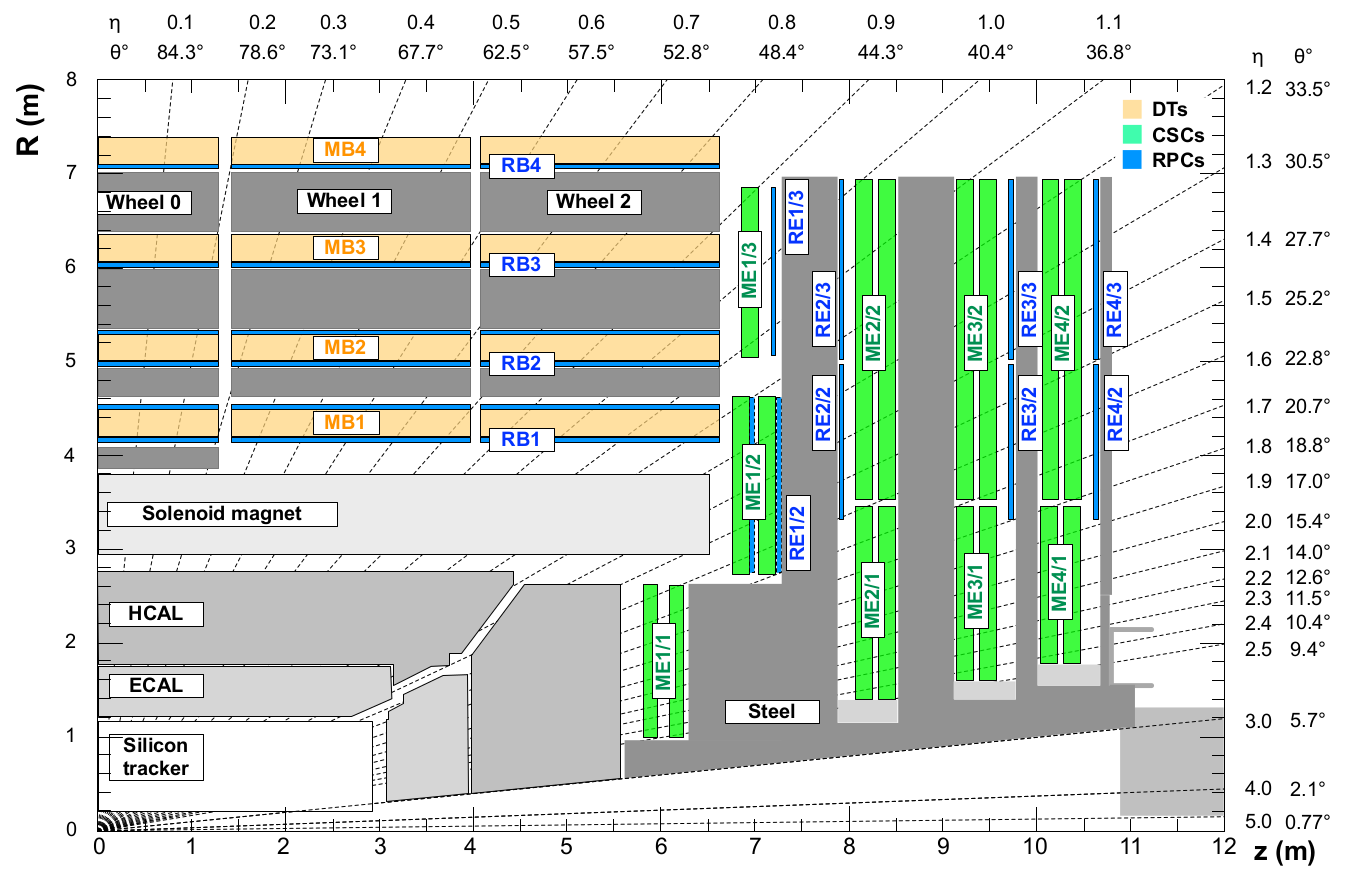
\includegraphics[width=\textwidth]{experiment/muonSystem.png}
  \caption[Muon system geometry]{
    Diagram of muon system and return yoke geometry, reproduced from Ref.~\cite{Abbiendi:2015txa}. The magnet, calorimeters, and inner tracker are also visible.
  }\label{fig:muonSystem}
\end{figure}


\subsubsection{Drift Tubes}
In the barrel ($\abseta < 1.2$), drift tube (DT) chambers are arranged in four ``stations'' separated by the steel layers of the yoke.
Stations are made of two or three superlayers (SLs) of four layers of rectangular drift cells.
Adjacent layers are staggered latterally by half a drift cell width to avoid gaps.
Each station has two SLs with wires running parallel to the beam to measure muon tracks in the $r$-$\phi$ plane, separated by an aluminum honeycomb lattice to provide mechanical rigidity and act as a spacer.
The inner three stations contain an extra SL on the outer side of the spacer with wires perpendicular to the beam line, to measure muon position along the $z$-axis.

Each drift cell contains a roughly $2.4\unit{m}$-long wire in gas (85\% Ar, 15\% CO$_2$).
The electric field in the cell is proveded by aluminum tape glued to the top and bottom of the cell and held at $+1.8\unit{kV}$ relative to the grounded aluminum plates above and below.
Aluminum tape cathodes on the side of the cell are held at $-1.2\unit{kV}$, while the wires act as $+3.6\unit{kV}$ anodes.
The width of each cell perpendicular to muon motion, $42\unit{mm}$, was chosen for a maximum drift time of $380\unit{ns}$, sufficient to obviate the need for double-hit readout logic in this low-occupancy region of the detector.
The height of $13\unit{mm}$ set by mechanical and space constraints.
Track timing resolution in each SL is a few nanoseconds when all cells are allowed to read out all deposited charge.
The $r$-$\phi$ position resolution available for online use in the trigger is about $1.5\unit{mm}$ in each SL\@; offline, for a single wire it is roughly $250\unit{\mu m}$, leading to an overall offline resolution of $100\unit{\mu m}$ at each station.


\subsubsection{Cathode Strip Chambers}
Muons with $1.2 < \abseta < 2.4$ are detected by the cathode strip chambers (CSCs).\footnote{Where the CSCs and DTs overlap ($0.9 < \abseta < 1.2$), tracks are formed from hits in both.}
The CSC system's trapezoidal chambers are arranged on discs interleaved with the endcap yoke in four layers.
Chambers close to the beamline each cover $20\degree$ sections in $\phi$ while outer chambers cover $10\degree$ sections, with overlap to avoid gaps.

A CSC chamber is made of seven panels sandwiched together to make six gaps filled with a gas mixture (40\% Ar, 50\% CO$_2$, 10\% CF$_4$).
Six of the plates have cathode strips milled into one side, varying in pitch from $8.4\unit{mm}$ at the narrow end of the trapezoid to $16\unit{mm}$ at the wide end, with $0.5\unit{mm}$ gaps between strips.
Three panels are wrapped with anode wires, alternating with the other panels so that every gas gap has a plane of wires.
Wires are spaced $3.2\unit{mm}$ apart and run azimuthally around the detector, except for the innermost chamber closest to the interaction point, which are inside the magnet and must have their wires tilted $29\degree$ so that charge collected by the wires moves parallel to them despite the Lorentz forces from the solenoid.

A typical muon will deposit charge in 3--4 cathode strips and a similar number of anode wires per gas gap, allowing hit position to be interpolated using all these signals as well as timing information.
The single-plane spatial resolution can be as good as $80\unit{\mu m}$ but depends strongly on where in the width of the strip the muon hits.
The strips in alternating planes are therefore offset by half their width.
Measurements from all six gas gaps in a chamber are combined into a segment with position resolution in the 30--$80\unit{\mu m}$ range, which depends on the chamber but not where in the chamber the muon hit.

Anodes and cathodes are held $3.6\unit{kV}$ from each other, leading to a drift time of roughly $300\unit{ns}$.
Single anode planes have an RMS timing resolution of around $11\unit{ns}$, insufficient for assigning a hit unambiguously to an individual bunch crossing, as required for triggering.
However, information from all six anode planes in a chamber can be combined to yield a segment timing resolution around $5\unit{ns}$.
Segments are therefore the unit of information sent to the trigger.
Segment position resolution at trigger level is 1--$2\unit{mm}$.


\subsubsection{Resistive Plate Chambers}
To provide a redundant set of muon momentum measurements, as well as precise timing of muon hits, CMS has six layers of resistive plate chambers (RPCs) in the barrel and four in the endcap up to $\abseta < 1.6$.
RPC chambers consist of two thin layers of intert gas (95.2\% C$_2$H$_2$F$_4$, 4.5\% C$_4$H$_{10}$, 0.3\% SF$_6$) each between a pair of Bakelite electrodes held at $9.3\unit{kV}$.
The two ``gas gaps'' are placed on either side of a plane of copper strips.
When a passing muon ionizes the gas, the high voltage causes a fast electron avalanche read out by the strips.
The narrow gap allows the RPCs to have single-hit timing resolution around $1\unit{ns}$, but the spatial resolution is limited to about $1\unit{cm}$ by the size of the readout strips.
The DTs and CSCs both have better momentum resolution than the RPCs, but RPCs are a simple, robust auxiliary system and the timing resolution can be used in conjunction with the other systems to improve overall muon measurements.
The gaps between RPC chambers do not align with the gaps in the other outer muon systems, increasing the muon spectrometer's geometrical acceptance.


\subsection{Data Acquisition and Trigger}
With a bunch crossing rate of $40\unit{MHz}$ and over 40 collisions possible in each crossing, the collision rate can exceed $1.6\unit{GHz}$.
Event sizes on disk of 1--$2\unit{MB}$ mean that the raw data generation rate of CMS could potentially be several PB/s, substantially more than can be read out, stored or analyzed with current technology.
However, most events consist only of low-energy, well-understood QCD interactions, so the data rate can be drastically reduced by reading out and storing only events likely to have interesting physics content.
CMS reduces the event rate with a two-level trigger system.

The level-1 (L1) trigger uses custom hardware operating on trigger primitives (TPs) containing lower-granularity detector information to reduce the event rate to $100\unit{kHz}$ or less.
The inner tracker's readout is too slow for use in the trigger, so only the calorimeters and muon systems generate TPs.
Events accepted at level-1 are fully read out, digitized, and sent to the high level trigger (HLT), where they are partially reconstructed in software and filtered further, reducing the final rate of stored events to roughly $1\unit{kHz}$.


\subsubsection{Level-1 Trigger}\label{sec:l1trig}
LHC beams collide at too high a rate for trigger decisions to be made in software, so the L1 trigger is instead implemented in custom hardware, with processing done using field-programmable gate arrays (FPGAs) as much as possible for flexibility, and application-specific integrated circuits (ASICs) where required.
Hardware limitations of other CMS subsystems---in particular, the inner tracker's readout speed and buffer capacity---impose strict constraints on the system.
The rate of events passing at level-1 cannot exceed $100\unit{kHz}$ and the system's overall latency cannot exceed roughly $4.2\unit{\mu s}$ from the proton-proton interaction to data storage at level-1.
These goals are achieved while maintaining high efficiency for interesting physics events by using low-granularity detector information, to reduce the bandwidth needed within the trigger system.
Information flows through several processing steps, with the data throughput reduced at each step.
Calorimeter and muon information are processed in parallel and combined only in the final step.
Optical links between systems provide high-bandwidth data transfer and allow flexibility in the overall trigger architecture.
The calorimeter trigger was upgraded with respect to the Run~I configuration in 2015, and the whole trigger system was overhauled in 2016~\cite{Tapper:1556311}.
Both configurations will be described here.

Calorimeter information is compressed into TPs for use in the trigger by trigger primitive generators (TPGs).
Each TP represents a ``tower'' consisting of a $5 \times 5$ cluster of barrel or endcap ECAL crystals and the HCAL tower behind them, or a section of the HF\@.
The TP contains an 8-bit transverse energy sum and a quality bit for each calorimeter, and six bits of error checking and bookkeeping information.
In 2015, TPs were sent to the Regional Calorimeter Trigger (RCT)~\cite{Chumney:2003ip}, which processed 18 portions of the detector (segmented in $\phi$ with $+\eta$ and $-\eta$ treated separately) in parallel in separate crates of electronics, using several ASICs and one FPGA in each crate for processing~\cite{Kreis:2015jjr}.
Each RCT crate summed the TPs with $\abseta < 3.0$ into $4 \times 4$ tower regions, and found isolated and non-isolated $2 \times 1$ tower $\Pe/\Pa$ and $\Pt$ candidates.
These objects were sent to Stage~1 Layer~2, which selected the best $\Pe/\Pa$ and $\Pt$ candidates from the entire detector, clustered regions into $3 \times 3$ region jet candidates, and computed global quantities like missing transverse energy and the scalar sum of transverse momentum for all particles in the event.
Pileup subtraction was performed with a lookup table (LUT) based on the number of regions in the detector with no energy.

In 2016, the whole calorimeter trigger was replaced with a new two-tiered system.
Stage~2 Layer~1 (``CaloL1'') consists of 18 FPGA-based Calorimeter Trigger Processor~7 (CTP7) cards~\cite{Svetek:C02011}, which calibrate and reformat the TPs before forwarding them to Stage~2 Layer~2 (``CaloL2'')~\cite{Kreis:2015jjr}, an FPGA-based time-multiplexed system which finds $\Pe/\Pa$, $\Pt$, and jet candidates and computes global quantities for whole events in parallel using tower-level information.

In 2015, the DTs and CSCs fed track segments into track finders (DTTF~\cite{Ero:2008zz} and CSCTF~\cite{Acosta:1999rpa}) which used pattern recognition algorithms to reconstruct tracks and measure their $\pt$, sharing information between the track finders to avoid inefficiency in the overlap region.
The RPCs made their own tracks.
Since the 2016 upgrade, track finding has been done by geometrical region of the detector rather than detector subsystem alone, with separate track finders for the barrel (BMTF, $\abseta < 0.85$) using DT and RPC information~\cite{Ero:2016vna}, the endcap (EMTF, $1.25 < \abseta < 2.4$) using CSC and RPC information~\cite{Tapper:1556311}, and the overlap region (OMTF, $0.85 < \abseta < 1.25$) using all three muon systems~\cite{Zabolotny:2016cik}.
The track finders feed into the Global Muon Trigger (GMT, upgraded to $\mu$GMT in 2016)~\cite{Sakulin:687846,Jeitler:2015stp}, which merges and sorts tracks, analyzes their quality and selects the best ones.

The calorimeter and muon trigger systems, which have up to this point worked entirely in parallel, both send their selected candidates and global quantities to the Global Trigger (GT, upgrated to $\mu$GT)~\cite{Jeitler:2007hn,Wittmann:C02029}.
The Global Trigger contains the trigger menu, the configurable set of algorithms used to determine whether an event is accepted or not.
These algorithms can use combinations of the objects from the calorimeter and muon trigger systems, including imposing topological requirements, e.g.\ requiring a large $\Delta\eta$ between muons in a pair.
The final decision is a logical OR of all triggers in the menu, but each trigger may be prescaled, i.e.\ only included in the final decision a fraction of the time in order to reduce its rate.
When an event is accepted, a level~1 accept (L1A) signal is sent to all CMS subsystems instructing them to read out information collected in the accepted event, which is stored in buffers until it can be read out or safely discarded.
A diagram of the whole 2016 L1 trigger system and its information flow is shown in Fig.~\ref{fig:triggerFlow}.

\begin{figure}[htbp]
  \centering
  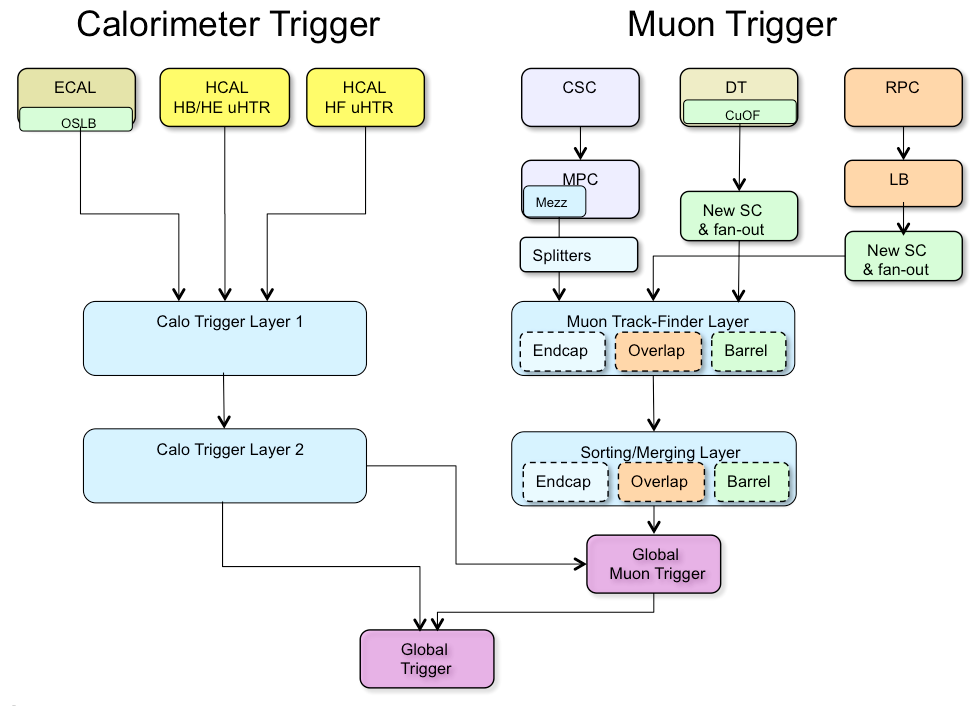
\includegraphics[width=\textwidth]{experiment/triggerFlow.png}
  \caption[Trigger data flow]{
    Data flow diagram for the CMS L1 trigger after the 2016 overhaul, reproduced from Ref.~\cite{Tapper:1556311}.
  }\label{fig:triggerFlow}
\end{figure}


\subsubsection{High-Level Trigger}
After an accepted event is read out and digitized, it must undergo another level of screening before being stored.
The High Level Trigger (HLT) uses full detector information reconstructed with versions of the normal CMS reconstruction algorithms specially optimized for speed, running on a large farm of commercial computers~\cite{Adam:2005zf}.
Much of HLT's power comes from having tracker information, allowing more precise momentum measurements, isolation calculations and identification algorithms than are available at L1.
For example, the pixels can be used to reconstruct vertices and tag $\Pqb$-quark jets, and requirements can be placed on the invariant mass of a lepton pair.
However, track reconstructions is slow, so it is typically only done as one of the last steps in the filtering process, allowing the event to be rejected based on more easily reconstructed objects like tracks in the muon system.
Other optimizations include only reconstructing tracks near objects passed in by the L1 Global Trigger.
The final result is that the rate of events saved for later analysis is around $1\unit{kHz}$.


\subsection{Luminosity Determination}
A precise measurement of the luminosity delivered by the LHC is critical to precisely measuring any cross section.
The instantaneous luminosity for $n_b$ colliding bunch pairs with intensity $N_b$ and orbit frequency $f_\textit{rev}$ is given by
\begin{equation}\label{eq:lumiByAeff}
  \lumiL = \frac{n_b N_b^2 f_\textit{rev}}{A_\text{eff}}
\end{equation}
where $A_\text{eff}$ is the effective area of the beam-beam overlap.
If beam $i$ has a gaussian density profile in the $u$ direction of width $\sigma_{i,u}$, and the beam densities are uncorrelated in each direction, then
\begin{equation}
  A_\text{eff} = 2\pi \sqrt{\sigma_{1,x}^2 + \sigma_{2,x}^2} \sqrt{\sigma_{1,y}^2 + \sigma_{2,y}^2}.
\end{equation}
The beam widths $\sigma_{i,u}$, the only unknowns in Eq.~\ref{eq:lumiByAeff}, are purely geometrical and can be found with the Van de Meer (VdM) scan method~\cite{vanderMeer:1968zz,Zanetti:1357856}.
In a VdM scan, for which LHC has a special run mode, one beam is held fixed while the position of the other is scanned in the $x$-$y$ plane, and detector activity is measured as a function of beam displacement.
Because the width of the interaction rate distribution is independent of its overall normalization, the detector activity metric may be any quantity linearly proportional to the interaction rate.

Over the course of an LHC run, $n_b$, $N_b$, and $A_\text{eff}$ are all subject to change, and in fact the VdM scans are performed regularly, so in practice the procedure outlined above provides a calibration and overall scale for luminosity measurements during physics collisions.
For a given detector metric labeled $Q$ with rate $R^Q$ that peaked at $R_0^Q$ with no beam displacement, the VdM scan yields a visible cross section, the constant of proportionality between the rate and the instantaneous luminosity,
\begin{equation}
  \sigma_\text{vis}^Q \equiv \frac{R^Q}{\lumiL} = A_\text{eff} R_0^Q.
\end{equation}
CMS has several such metrics; the primary one used for measuring integrated luminosity is the number of pixel hit clusters~\cite{CMS-PAS-LUM-15-001,CMS-PAS-LUM-17-001}.
The instantaneous luminosity is given by
\begin{equation}
  \lumiL = \frac{\langle N_c \rangle f_\textit{rev}}{\sigma_\text{vis}^\text{PCC}} = \frac{\langle N_c \rangle}{A_\text{eff} \langle N_c \rangle_0}
\end{equation}
where $\langle N_c \rangle$ is the average number of pixel hit clusters at each bunch crossing and $\langle N_c \rangle_0$ is its peak value during the VdM scan.

A number of complications must be accounted for or included in systematic uncertainty estimates.
Beam-beam interation effects, correlations between the proton density distributions in the $x$ and $y$ directions, drifts in the beam orbit, and normalization uncertainties on the bunch intensity and absolute distance scale from the beam spot must all be handled with care.
The result is a total integrated luminosity uncertainty of $2.3\%$ in 2015 and $2.5\%$ in 2016\@.

%!TEX root = ../nwoods_thesis.tex

\chapter{Simulation}\label{ch:simulation}

\section{Monte Carlo Event Generation}
It's like gambling

\subsection{Matrix Element Generation}
The real physics


\subsection{Parton Shower, Hadronization, and Underlying Event}\label{sec:partonShower}
The way-too-real physics


\subsection{Pileup Simulation}
Lots of it



\section{Detector Simulation}
All kinds of fun

%!TEX root = ../nwoods_thesis.tex

\chapter{Object Reconstruction and Selection}

The raw detector information stored on disk after an event passes trigger selections is not yet suitable for physics analysis.
Hits in the tracker and muon systems, and energy deposits in the calorimeters, require significant processing to build physics objects that are interpretable in terms of the physics of the hard scatter.
Patterns in the tracker and muon system hits are found and used to construct charged particle and muon tracks, and energy deposits in the calorimeters are grouped into clusters.
Final state particles that interact with CMS are reconstructed from the tracks and calorimeter clusters, final state particles are clustered into jets, charged particles are clustered by track origin to find proton-proton collision vertices, and visible particle momenta are summed to find the transverse momentum imbalance from undetectable particles (e.g.\ neutrinos).
The resulting physics objects undergo selection to determine which represent real particles of interest for the analysis.
Selected particles are used to reconstruct the hard interaction from the collision---in the analyses presented here, leptons are paired to form $\PZ/\Pa^\ast$ boson candidates which may be paired to form Higgs or {\PZ} boson candidates, and jets are used to distinguish electroweak and QCD {\ZZ} production.


\section{Track Reconstruction and Vertex Identification}\label{sec:trkVtxReco}

Tracks are reconstructed in the inner tracker by iterative application of a combinatorial Kalman filter algorithm~\cite{Fruhwirth:1987fm,Billoir:1990we,Adam:2005cg,Chatrchyan:2014fea}.
At each iteration, tracks found in the pixel detector are used as ``seeds'', track segments which serve as the initial trajectories on which strip tracker hits from the same particle are expected.
The pixel seed supplies the initial parameters for the combinatorial Kalman filter.
At each tracker layer, the algorithm predicts where the particle will hit the next layer based on the track's current parameters, taking into account the effects of particle interaction with tracker material.
The extrapolated trajectory is used to find compatible hits in the next layer with a $\chi^2$ test, and if possible the most compatible hit is added to the track and its parameters are updated accordingly.
If no hits are compatible, a ``ghost'' hit which does not contribute to the track parameters may be added to account for the possibility of a missing hit in the corresponding layer.
This procedure is repeated recursively at each tracker layer, from the innermost layer past the seed to the outermost layer of the silicon strip tracker.
If two tracks found in an iteration share too many hits, they are assumed to be from the same particle and the one with fewer hits is rejected, using the total $\chi^2$ of all hits as a tiebreaker.
The first iterations of the track finding algorithm searches for high-$\pt$ tracks from primary proton-proton interactions, which are easier to find because they are close to straight and originate from the beam line.
When a track is found, its constituent hits are removed from consideration in future iterations, reducing the computational complexity of finding the more difficult tracks from lower-$\pt$ particles and products of $\Pqb$~hadron decays which happen away from the beam line.

Because the Kalman filter obtains the final track parameters only at the outermost tracker layer, each track is refit and smoothed with further Kalman filters, improving track quality and reducing fake rate.
Spurious tracks are rejected from the final collection with requirements on the number of layers hit, the $\chi^2$ of the fit, and compatibility with a primary vertex.LHC
The efficiency for reconstructing tracks of all prompt charged particles with $\pt > 900\MeV$ is around 94\% in the barrel and 85\% in the endcap; for isolated muons, it is virtually 100\% in the whole tracker acceptance~\cite{Chatrchyan:2014fea}.

Electrons lose substantially more energy to interactions with the tracker material than other charged particles, often breaking the assumption of Gaussian energy loss inherent to the Kalman filter.
To mitigate the impact of the resulting poor track fits, tracks with many missing hits or a poor $\chi^2$ are refit using a Gaussian sum filter (GSF)~\cite{Adam:2005bya}.
Any Kalman filter or GSF tracks with trajectories that intersect ECAL energy clusters (see below) are considered electron track candidates and refit with a second, more complicated GSF\@.
This GSF track collection is used as inputs to the PF electron reconstruction described below.

Proton-proton interaction vertices are found by clustering tracks by minimizing the figure of merit
\begin{equation}\label{eq:vtxChi2}
  \chi^2 = \sum_i \sum_j p_{ij} \frac{\left(z^t_j - z^V_i\right)^2}{\sigma_{j}^2},
\end{equation}
where $z^V_i$ is the $z$ position of vertex $i$, $z^t_j$ is the $z$-axis position of track $j$ at its closest point to the beamline and $\sigma_j^2$ is its uncertainty.
The track-vertex association matrix $p_{ij}$ maps tracks to their associated vertices, i.e.\ $p_{ij} = 1$ if vertex $i$ and track $j$ are associated, $p_{ij} = 0$ if they are not.
Rather than minimize Eq.~\ref{eq:vtxChi2} directly with an unknown number of vertices, the CMS clustering algorithm~\cite{Speer:2006mh,Chatrchyan:2014fea} uses a technique known as deterministic annealing~\cite{Rose:726788}, which treats the system as a statistical ensemble of associations between the tracks and an unknown number of vertices.
The association matrix $p_{ij}$ is then the probability that vertex $i$ and track $j$ are associated.
If every possible set of assignments, for every possible number and arrangement of vertices, is considered equally probably, this is analogous to a thermodynamic system at high temperature, with $\chi^2$ playing the role of energy.
The system is simulated at high ``temperature'' and the analog of free energy is minimized to determine $p_{ij}$.
The temperature is then lowered in steps, with track-vertex associations deterministic in the limit of zero temperature.

Among the interaction vertices in an event, the one whose associated charged particles have the highest sum of $\pt^2$ is labeled the primary vertex (PV).
A PV must be less than 24\unit{cm} from the nominal beam spot in the $z$ direction and less than 2\unit{cm} from the beamline.



\section{Particle Flow Reconstruction}

The simplest conceivable algorithm would reconstruct each type of particle mostly with information from single subsystems: muons with the outer muon system, electrons and photons with ECAL, jets with the calorimeters aided by inner tracker information to handle $\Pqb$ jet vertexing, etc.
This approach is sufficient for many analyses and sophisticated versions of the general principle have performed admirably at a number of experiments, but it is suboptimal.
It fails to exploit the full detector information for many objects---for example, not using the inner tracker's precise measurements of low-energy charged hadrons in jets made by clustering calorimeter deposits---and misses significant correlations between detector systems.
The CMS collaboration takes a different approach, using a particle flow (PF) algorithm combining subdetector signals for optimal particle reconstruction and identification~\cite{CMS:2009nxa,CMS:2010byl,Sirunyan:2017ulk}.

Several features of CMS facilitate PF reconstruction, as described in Section~\ref{sec:cms}.
The most important is that the calorimeters are inside the magnet and close to the tracker, so charged particles are much less likely to interact with material between them.
The inner tracker's precise position measurement and ECAL's fine segmentation thus allow tracks to be associated to calorimeter clusters even for individual charged hadrons of modest energy.

\subsection{PF Candidates}

The inputs to the PF algorithm are inner tracker tracks, muon system tracks, and clusters of energy deposits in the calorimeters, all of which are calibrated beforehand.
Calorimeter clusters are built independently for each subsystem, with ECAL and HCAL barrel and endcaps considered separately.
Topological clusters are built by combining adjacent cells with energy deposits over a threshold, using cells that are local energy maxima as seeds.
Within the topological clusters, the final calorimeter clusters are built by fitting the energy deposits with the sum of several two-dimensional Gaussians, one Gaussian for each seed in the topological cluster.

The first step of the PF algorithm is to link tracks and clusters across subdetectors.
Tracks are linked to calorimeter clusters by extrapolating from the track to the calorimeter cells the particle would be expected to hit.
To account for bremsstrahlung photons from electron interactions with tracker material, GSF tracks are linked with ECAL clusters compatible with a tangent to the track where it hit the tracker.
Overlapping ECAL and HCAL clusters are linked outside the inner tracker acceptance.
Inner tracks are linked to muon system tracks if they are compatible with each other within the resolution of the muon system.
The groups of linked objects, called ``PF blocks'', usually originate from one or a few particles and are the basic unit of PF reconstruction.

\subsubsection{Muons}

Muon candidates in CMS~\cite{Chatrchyan:2012xi} come in three flavors: ``standalone'', ``tracker'', and ``global'' muons.
Standalone muons use only the track from the muon spectrometer (the ``standalone track''), built with a fit to track segments made of clusters of hits in the DTs, CSCs, and RPCs.
Tracker muons use only the inner track, identified as a muon because the track is compatible with one or more track segments in the muon system.
Global muons use a combined ``global track'' made by fitting the hits in an inner track and a compatible standalone track to a common muon trajectory through the whole detector.
By construction, global muons have corresponding standalone and tracker muons.
The inner track typically dominates the global track fit, so the corresponding tracker muon is merged with the global muon.
When a muon candidate is reconstructed, its constituent tracks are removed from the PF block and are therefore not used in further reconstruction.

\subsubsection{Electrons and Prompt Photons}

Electron reconstruction uses GSF tracks linked with ECAL clusters~\cite{Baffioni:2006cd,Adam:2005bya}.
The cluster associated to a track and the bremsstrahlung candidate clusters on tangents to the track are collectively called the ``supercluster''.
Prompt photons are reconstructed from superclusters without associated tracks except displaced track pairs consistent with $\Pa \to \Pe^+\Pe^-$ conversions in the tracker material~\cite{Khachatryan:2015iwa}.
In both cases, the HCAL energy near the supercluster cannot be more than 10\% of the supercluster energy.
Non-isolated photons, i.e.\ those with substantial nearby tracks or calorimeter deposits or a ratio of ECAL and HCAL energy incompatible with a photon, as assumed to be from $\pi^0$ decays and are described with neutral hadrons in the next section.
Tracks and clusters used to reconstruct electrons and photons are removed from the PF block and are not used in hadron reconstruction.

\subsubsection{Charged and Neutral Hadrons}

With muon, electron, and prompt photon constituents removed, remaining detector signals are taken to be from charged and neutral hadrons (including non-prompt photons)~\cite{CMS:2009nxa,Sirunyan:2017ulk}.
Clusters in ECAL without associated tracks are taken to be photons from $\pi^0$ decays, because neutral hadrons deposit very little energy in ECAL\@.
Trackless clusters in HCAL are taken to be neutral hadrons.
Both are removed from the PF blocks, so all that remain are linked clusters and tracks.
Paired tracks and clusters with compatible energies are taken to be charged hadrons.
If the track {\pt} is much less than the calorimeter-measured {\pt}, the pair is labeled as overlapping charged and neutral hadrons.


\subsection{Jets}

Effective clustering of hadrons, non-prompt photons, and non-prompt leptons into jets is critically important for many physics analyses, including the $\ZZ + \text{jets}$ differential cross section measurements and the {\ZZ} VBS search.
Clustering must be efficient, to ensure the tagging jets in VBS events are found, but the clustering algorithm should not tag spurious jets, as the number of jets in an event is sensitive to higher-order QCD corrections and therefore an interesting quantity to compare to theoretical predictions.
Similarly, the algorithm should not erroneously cluster particles from the same initial parton into multiple jets or merge jets from multiple original partons, because the kinematics of the original quarks and gluons are also of theoretical interest and the detector-level jet kinematics should accurately reflect them.
A clustering algorithm is said to be ``infrared safe'' if the presence of low-energy hadrons from soft gluon radiation does not change the number of jets or have a qualitatively significant effect on jet shapes and kinematics.
This fits with the intuition that a single {1\GeV} pion should have essentially no effect in an event with multiple jets with energies on the order of hundreds of {\GeVns}~\cite{Salam:2007xv}.
An algorithm is said to be ``collinear safe'' if the jets are not changed substantially by splitting one hadron into two nearly collinear hadrons with the same total four-momentum.
This also fits with physical intuition in that jets deposit energy over an area significantly larger than the spatial resolution of the detector, so increasing the detector granularity enough to resolve two very close particles (without changing their total four-momentum) should have little or no effect on the jet.

Infrared and collinear (IRC) safety are critically important for comparing data to theoretical predictions~\cite{Salam:2009jx}.
Collinear splittings and soft gluon radiation during jet fragmentation should not affect the dynamics of the {\TeVns}-scale hard scattering processes we wish to probe, but they are nonperturbative and difficult to model, and experimental analysis can only probe the underlying hard interaction if it is insensitive to this kind of mismodeling.
Experimental detectors' finite resolution and inability to measure arbitrarily soft particles enforces some level of IRC safety on any algorithm, but the results of an analysis methods that uses an IRC unsafe clustering will depend on the complex, detector-dependent details of this partial IRC regularization.
In any case, the most meaningful comparisons between data and theory should use the same definition of a jet in the experimental analysis and the perturbative calculation, and perturbative calculations require IRC safe observables to preserve unitarity.

These considerations, and the desire for conical jets with a well-defined area in the $\eta$-$\phi$ plane, lead most CMS analyses (including this one) to use jets clustered with the anti-{\kt} algorithm~\cite{Cacciari:2008gp,Cacciari:2011ma}.
The anti-{\kt} algorithm defines the distance between two particles $i$ and $j$ as
\begin{equation}
  d_{ij} = \min\left(p_{\text{T}i}^{-2}, p_{\text{T}j}^{-2}\right) \frac{\Delta_{ij}}{R},
\end{equation}
where $\Delta_{ij}$ is the distance in the rapidity-polar angle plane,
\begin{equation}
  \Delta_{ij}^2 \equiv \left(y_i - y_j\right)^2 + \left(\phi_i - \phi_j\right)^2,
\end{equation}
and $R$ is a parameter setting the size of the resulting jets.
The algorithm proceeds iteratively.
At each iteration, if the smallest $d_{ij}$ between any pair of particles in the event is smaller than the smallest $\pt^{-2}$ of any single particle, the particles in the pair are merged into a single particle with their total four-momentum.
If the minimum single-particle $\pt^{-2}$ is smaller than the minimum $d_{ij}$, the single particle is labeled a jet and removed from further consideration.
Iteration proceeds until all particles are part of a jet.
In this analysis, the size parameter used is $R = 0.4$.

Charged hadrons from pileup interactions are not included in jet clustering~\cite{CMS:2014ata}.
The contribution of neutral hadrons from pileup is estimated with a jet area technique~\cite{Khachatryan:2016kdb,Cacciari:2008gn,Cacciari:2007fd} in which the energy density of neutral hadrons from pileup is calculated event-by-event and multiplied by the area of the jet to estimate the neutral pileup contribution, which is subtracted from the jet energy.
Jets in Monte Carlo samples have their energy shifted and stochastically smeared such that the overall energy scale and resolution match that of jets in data~\cite{Chatrchyan:2011ds,Khachatryan:2016kdb}.


\subsection{Missing Transverse Energy}

Neutrinos---or, hypothetically, WIMP dark matter or other new particles that do not decay or interact directly with the detector---escape and cannot be directly measured.
Because the beams have no momentum in the $x$-$y$ plane, the transverse momentum of the visible particles must balance the transverse momentum of the invisible ones.
The missing transverse momentum is thus
\begin{equation}\label{eq:MET}
  \ptvecmiss = -\! \! \sum_\text{visible} \ptvec,
\end{equation}
where the sum runs over the transverse momenta of all PF candidates in the event.
The missing transverse energy, {\MET}, is its magnitude.
The {\MET} is calibrated by propagating the jet energy scale corrections to the {\MET} calculation~\cite{Chatrchyan:2011tn,Khachatryan:2014gga,CMS-PAS-JME-16-004}.
PF candidates originating from pileup interactions are included in the sum in Eq.~\ref{eq:MET} because these soft collisions are very unlikely to produce neutrinos, so including them biases the measurement less than trying to determine which neutral particles should be considered pileup and which should not.
The charged tracks from pileup events are used to correct for the residual bias arising from the slightly lower efficiency for soft neutral particles from pileup.



\section{Object Identification and Selection}

The reconstruction algorithms described above are general purpose in the sense that they can be used in nearly any analysis, but do not address the specific needs of any, so further selections are essentially always required to optimize object efficiency and purity for studying a specific physics process.
The leptons used in this analysis are required to pass identification requirements on top of those imposed during PF reconstruction, and are required to be isolated from other particles in the event, to reject fake objects from jet fragmentation.
Four-lepton processes have low reducible backgrounds, so the selections presented here are generally loose, optimized for high efficiency compared to most CMS analyses.


\subsection{Electrons}

Electrons are required to have $\pt > 7\GeV$ and to be in the tracker acceptance, $\abseta < 2.5$.
They must be compatible with the PV, with minimum track-PV distance $d_z < 1\unit{cm}$ in the $z$ direction and $d_{xy} < 5\unit{mm}$ in the plane transverse to the beam.
Each electron's 3-dimensional impact parameter (IP) $d_\text{3D}$ must satisfy a requirement on its significance,
\begin{equation}
  \text{SIP}_\text{3D} \equiv \frac{d_\text{3D}}{\sigma_{d_\text{3D}}},
\end{equation}
where $\sigma_{d_\text{3D}}$ is the uncertainty on the IP\@.
The $\text{SIP}_\text{3D}$ requirement is $\text{SIP}_\text{3D} < 10$ for the {\ZZ} and $\PZ \to 4\ell$ cross section measurements and the aTGC search, and $\text{SIP}_\text{3D} < 4$ for the Higgs boson measurement and the VBS and aQGC searches.
To remove fake electrons arising from muon tracks being associated to photons or other incidental ECAL energy clusters, electrons within $\Delta R < 0.05$ of a muon are vetoed.

To further reduce photon and jet fragment backgrounds while maintaining high prompt electron efficiency, a further selection is applied using a multivariate discriminator made with a boosted decision tree (BDT)~\cite{CMS:2010bta,Khachatryan:2015hwa}.
The BDT uses 21 input variables, which fall into three broad categories:
\begin{itemize}
  \item Track-related observables like the number of hits and normalized $\chi^2$ of the Kalman and GSF tracks and the energy lost to bremsstrahlung according to the GSF fit. These are intended to discriminate between electrons and charged hadrons.
  \item Calorimetric information including a number of supercluster shape observables and the amount of HCAL energy near the supercluster, to discriminate electrons from electromagnetically rich jets.
  \item Track-cluster observables comparing the positions and momenta of the particles seen in the tracker and by ECAL\@.
\end{itemize}
The BDT training and working point selection are done separately for electron candidates with {\pt} above and below {10\GeV} and in three bins of {\abseta} (0--0.8, 0.8--1.479, and 1.479--2.5).
The working points are chosen to correspond to 98\% efficiency for single signal electrons in each bin.

To ensure that electron candidates are not part of a jet, they are required to be isolated from other particles in the event.
The relative isolation is defined as
\begin{equation}\label{eq:iso}
  R_\text{Iso} = \left( \sum_\text{charged} \! \!\pt + \max\left[0, \sum_\text{neutral} \! \!\pt + \sum_{\text{photons}} \! \!\pt - \pt^\text{PU} \left(\ell\right) \right]\right) \bigg/ \pt^{\ell}
\end{equation}
where the sums run over the {\pt} of PF hadrons and photons in a cone of $\Delta R < 0.3$ around the electron trajectory.
To mitigate the contribution of pileup to the isolation calculations, charged hadrons are included only if they originate from the event's PV\@.
The estimated neutral contribution to isolation from pileup, $\pt^\text{PU}\left(\ell\right)$, is defined for electrons as
\begin{equation}
  \pt^\text{PU}\left(\Pe\right) \equiv \rho \times A_\text{eff},
\end{equation}
where the average transverse-momentum flow density $\rho$ is calculated in each event using the jet area method described above.
The effective area $A_\text{eff}$ is the geometric area of the isolation cone times an $\eta$-dependent correction factor that accounts for the residual dependence of the isolation on pileup.
Electrons are considered isolated if their relative isolations satisfy $R_\text{iso} <0.35$.

Efficiencies for GSF track reconstruction, electron reconstruction and identification, and electron isolation criteria, are found with a ``tag-and-probe'' method~\cite{CMS:2011aa}.
In this technique, events are selected which contain at least one high-{\pt} ``tag'' electron passing strict ID and isolation requirements, and a ``probe'' track with the opposite sign that combines with the electron to have an invariant mass close to the {\PZ} boson mass.
The resulting sample is enriched with $\PZ \to \Pe^+\Pe^-$ events, so the track is likely to correspond to a real prompt electron.
Unlike all background processes, $\PZ \to \Pe^+\Pe^-$ production forms a distinct resonance peak in the $m_{\ell\ell}$ distribution, so shape fits can be used to find the overall purity of the sample, and thus the number of prompt electrons among the probes.
The selection efficiency is then the number of passing probes divided by the total number of prompt probes.
This procedure is performed in bins of {\pt} and $\eta$ for data and Monte Carlo events, and residual differences in efficiency in Monte Carlo samples are corrected to match data by weighting events by the ratio of data and Monte Carlo efficiency for each electron candidate.


\subsection{Muons}

Muon selection is similar to electron selection, but simpler because muon backgrounds are much smaller.
Candidate muons are required to be tracker or global muons with $\pt > 5\GeV$  within the muon system acceptance ($\abseta < 2.4$).
They are subject to the same PV compatibility criteria as electrons, $d_z < 1\unit{cm}$, $d_{xy} < 5\unit{mm}$, and $\text{SIP}_\text{3D} < 10$ or 4 depending on the analysis.
Muon candidates are further subject to the so-called ``PF ID'' criteria, which require them to be isolated from calorimeter deposits or to have high-quality tracks with good fits~\cite{Sirunyan:2017ulk}.

Isolation is defined as in Eq.~\ref{eq:iso}, the same as for electrons except for the definition of the neutral pileup contribution, which for muons is based on using the known charged pileup density to estimate the neutral pileup based on the average charge composition of pileup jets,
\begin{equation}
  \pt^\text{PU}\left(\Pm\right) \equiv 0.5 \sum_\text{charged} \pt^\text{PU},
\end{equation}
where the sum runs over the charged particles from all pileup vertices.
As for electrons, the radius of the isolation cone is 0.3 in the $\eta$-$\phi$ plane and the selection criterion is $R_\text{iso} < 0.35$.
Muon efficiencies are measured and corrected with the same tag-and-probe technique as used for electrons.


\subsection{Jets}

Jets are considered for analysis if they have $\pt > 30\GeV$ and $\abseta < 4.7$.
Loose criteria are applied to reject spurious jets by requiring they contain multiple particles, and the particles be a mix of charged and neutral consistent with hadronic jets.
Jets are removed from consideration in the event if a lepton or FSR photon is in its cone ($\Delta R < 0.4$).


\subsection{Final State Photon Radiation}

Final-state radiation (FSR) photons emitted by muons are not included in the PF momentum reconstruction, and some photons emitted by electrons may be missed, degrading {\PZ} boson reconstruction.
Photons are considered FSR candidates if they have $\pt > 2\GeV$, $\abseta < 2.4$, relative isolation $R_\text{iso} < 1.8$ as defined in Eq.~\ref{eq:iso} (with no neutral pileup correction), and $\Delta R \left(\ell, \gamma \right) < 0.5$ with respect to the nearest lepton.
To avoid double counting, photons in electron superclusters are not considered.
Because FSR has a higher energy spectrum than photons from pileup and is expected to be quasi-collinear with the emitting leptons, a photon is accepted as FSR and included in the \ZZ final state if $\frac{\Delta R \left( \ell, \gamma \right)}{{\et}_\gamma^2} < 0.012$.
FSR photons are omitted from the isolation determination for emitting leptons.
In the rest of this thesis, the momentum of any FSR photons found is included in $\PZ/\Pa^\ast$ and {\ZZ} four-momenta unless otherwise stated.



\subsection{Misidentified Objects}\label{sec:looseID}
Fake rates



\section{ZZ Candidate and Event Selection}
Explain the different classes of events (full spectrum, Higgs, on shell\ldots)

\subsection{Z Candidate Selection}\label{sec:zSelection}
Mass cuts and lepton pairing


\subsection{ZZ Candidate Selection}
Disambiguation for $>4$ leptons


\subsection{Background Estimation}


\subsection{VBS Signal Selection}\label{sec:vbsSelection}
Dijets and so on

%!TEX root = ../nwoods_thesis.tex

\chapter{Analysis Strategy}\label{ch:methods}

Four-lepton signal processes are generally well modeled, and backgrounds are small, so most analyses can use simple ``cut and count'' comparisons between data and Monte Carlo samples' yields after applying the selections described in Chapter~\ref{ch:reco}.
The comparisons include the contribution from reducible backgrounds, which is estimated with a data-driven technique.
Inclusive and differential cross sections are extracted from the observed yields with maximum likelihood estimation techniques.
The search for vector boson scattering extracts the signal yield with a multivariate discriminator, and the searches for anomalous couplings use a profile likelihood method to extract limits from the bin-by-bin yields in the $m_{4\ell}$ distribution.
These techniques are all described in this chapter, as are the relevant systematic uncertainties, which are taken into account by varying the input parameters to the yields and observing the resulting changes in yield and spectrum shape.



\section{Background Estimation}\label{sec:bkg}

Reducible backgrounds for four-lepton events typically have two or three prompt leptons and two or one other objects---typically jet fragments, sometimes photons---which are misidentified as prompt leptons.
The largest source of background contamination is from events in which a {\PZ} boson is produced in association with a photon and a jet, a leptonically-decaying $\PW$ boson and a jet, or two jets.
There is also a contribution from {\TTbar} events in which both top quarks decay to a lepton, a neutrino, and a {\Pqb}~quark jet.
For simplicity, the two sets of processes are not treated separately in what follows, and are collectively labeled ``$\PZ+\PX$'' events\footnote{This is a bit of a misnomer, as ``$\PZ+\PX$'' does not accurately describe {\TTbar} events, but the terminology is retained here for consistency with the CMS papers on these analyses.}.

The contributions of the reducible backgrounds to the selected four-lepton signal samples are evaluated using the tight-to-loose ``fake rates'' method, described in Ref.~\cite{Chatrchyan:2013mxa}.
In this procedure, the likelihood of a nonprompt (``fake'') object to be misidentified as a prompt lepton is estimated and applied to control regions enriched with $\PZ+\PX$ events to estimate their contribution to the signal region.
The lepton misidentification rate $f_\ell\left(\pt^\ell, \eta^\ell\right)$ is measured from a sample of $\PZ + \ell_\text{fake}$ events, where the {\PZ} boson candidate is selected as in the signal region but with $\left| m_{\ell\ell} - m_\PZ \right| < 10\GeV$, and the $\ell_\text{fake}$ object is a lepton candidate that passes relaxed ID requirements as defined in Section~\ref{sec:looseID}, with no isolation or tight ID requirements applied.

The misidentification rate is defined as the fraction of $\ell_\text{fake}$ candidates which pass full lepton identification and isolation critera, in bins of $\pt$ and $\eta$.
One should note that the misidentification rate cannot be interpreted as a probability in the usual sense, and if fact there is no simple physical interpretation of it.
Events with three prompt leptons can contaminate this control region and bias the misidentification rate, because the {non-\PZ} lepton is falsely assumed fake.
To mitigate this bias, the $\WZ \to 3\ell\nu$ yields in the numerator and denominator in each bin are estimated from a simulated sample and subtracted before the ratio of yields is taken.
Figure~\ref{fig:fakerates} shows the misidentification rates for electrons and muons separately as a function of {\pt} and $\eta$.

\begin{figure}[htbp]
  \begin{center}
    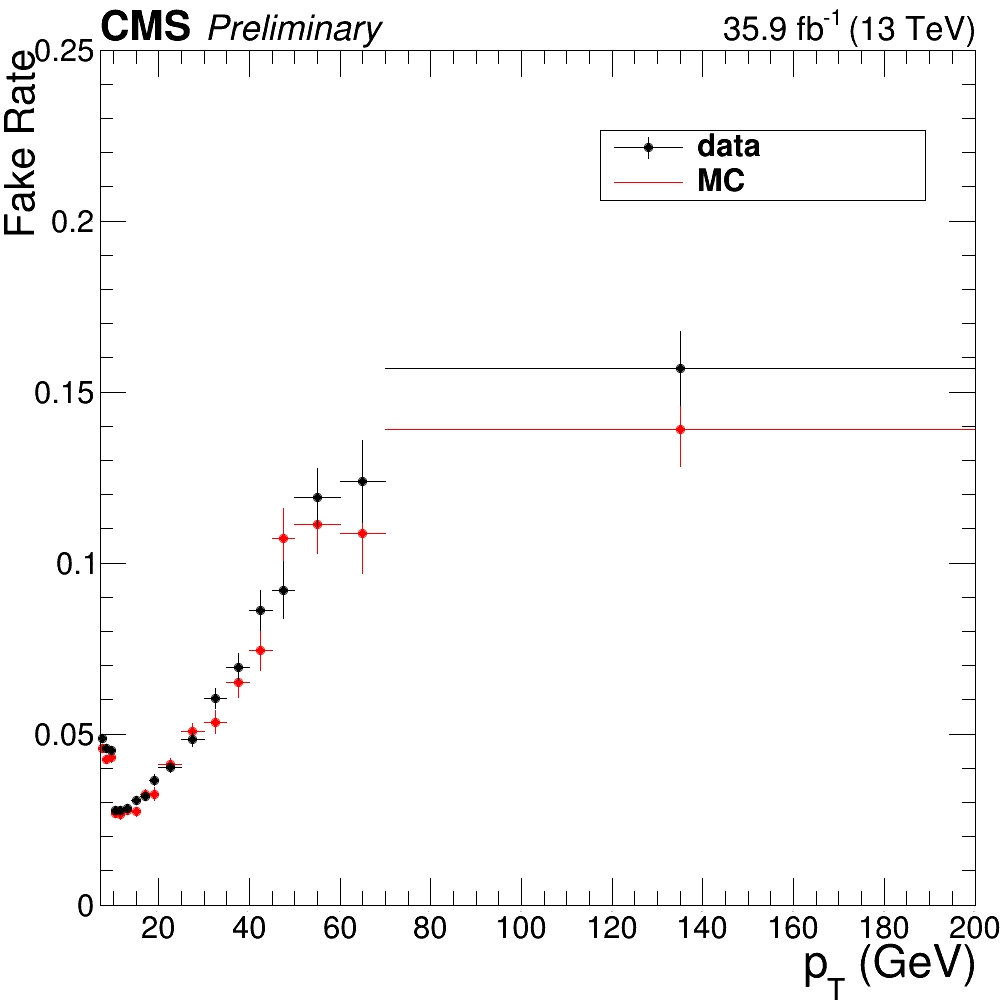
\includegraphics[width=0.35\textwidth]{methods/eFakeRate_pt.png}
    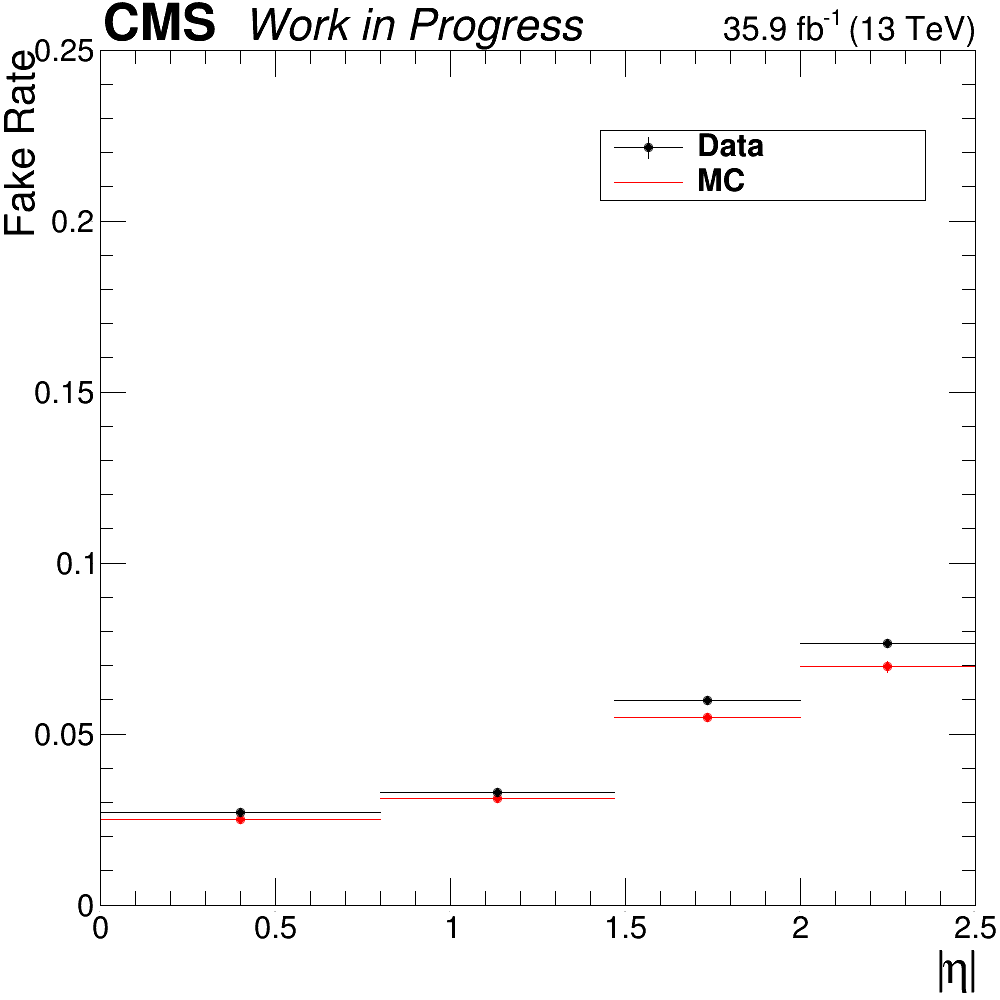
\includegraphics[width=0.35\textwidth]{methods/eFakeRate_eta.png} \\
    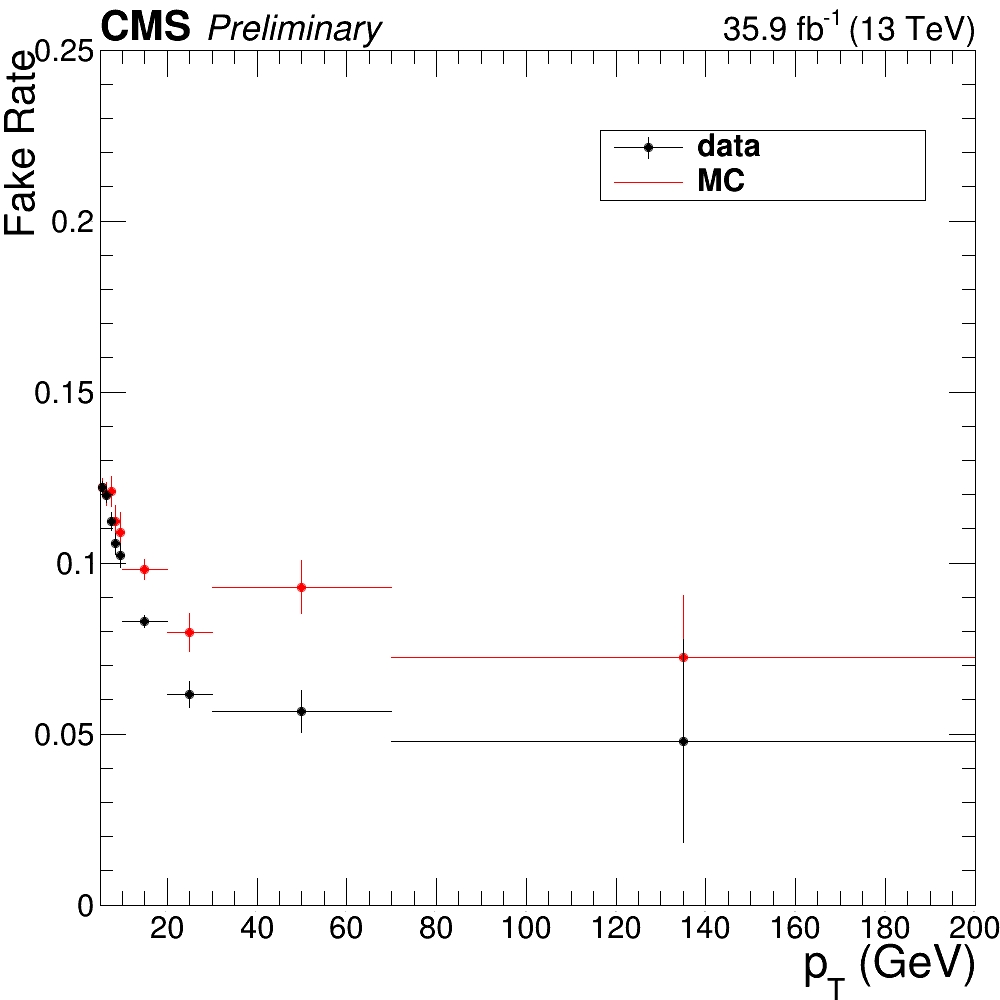
\includegraphics[width=0.35\textwidth]{methods/mFakeRate_pt.png}
    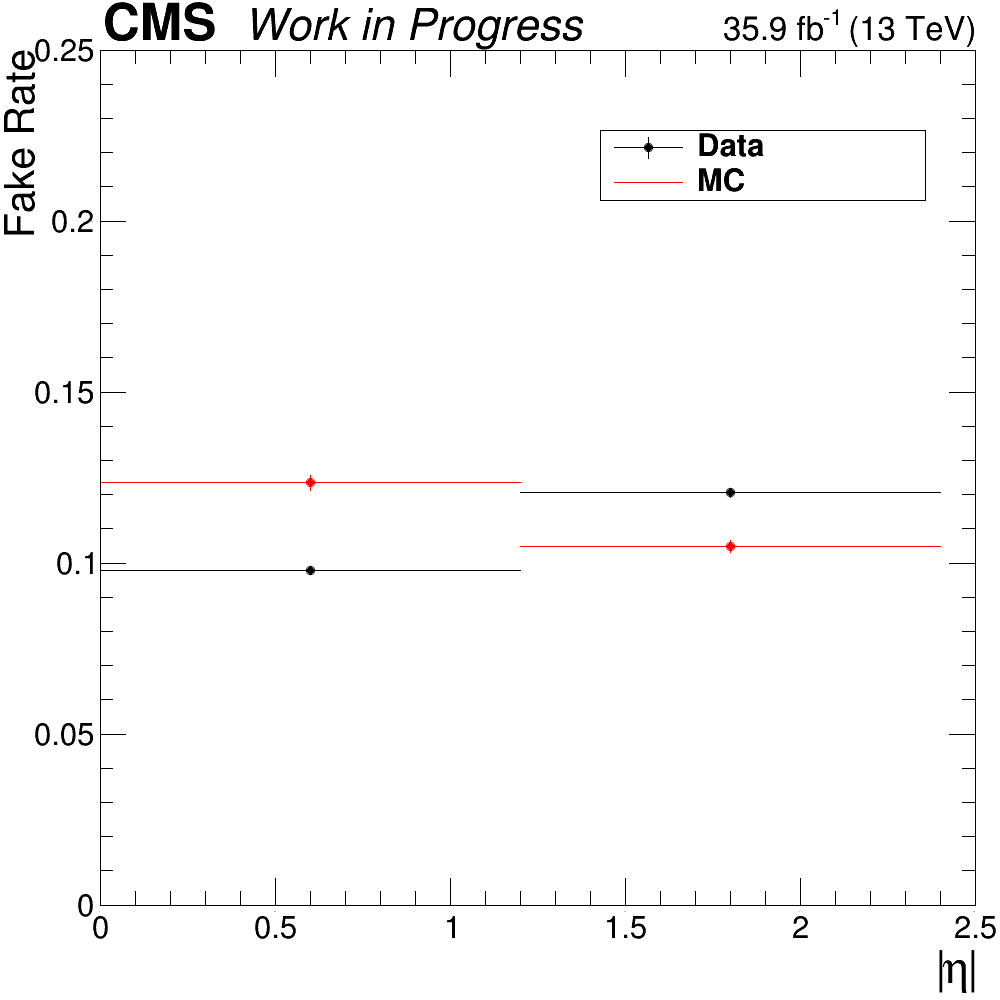
\includegraphics[width=0.35\textwidth]{methods/mFakeRate_eta.png}
    \caption[Misidentification rates for electrons and muons]{
      Fake rate for electrons~(top) and muons~(bottom) as a function of $\pt$~(left) and $\eta$~(right).
      }\label{fig:fakerates}
  \end{center}
\end{figure}

To estimate the total reducible background yield, the misidentification rates are applied to two $\PZ+\PX$ enriched control samples, each containing a {\PZ}~boson candidate passing all signal region requirements plus two more lepton candidates which pass the relaxed identification criteria and would make a second {\PZ} boson candidate according to Section~\ref{sec:zSelection} except that one or both fail the full identification or isolation criteria.
The sample with one failing lepton, called the ``3P1F'' sample for ``3 prompt 1 fake,'' covers the contribution from {\WZ} events, while the sample with both leptons in the second {\PZ} boson failing (``2P2F'') covers $\PZ+\text{jets}$, $\PZ\Pa+\text{jets}$, and {\TTbar} events.
The fake object transfer factor
\begin{equation}
  F_\ell\left(\pt^\ell,\eta^\ell\right) = \frac{f_\ell\left(\pt^\ell, \eta^\ell\right)}{1 - f_\ell\left(\pt^\ell, \eta^\ell\right)}
\end{equation}
is the ratio of nonprompt objects passing the relaxed and full selection criteria, and thus serves as a per-lepton extrapolation factor between control sample yields and signal sample yields.

The total reducible background yield is thus
\begin{equation}\label{eq:bkgYield}
  N_\text{bkg} = \sum_{\ell \in \text{3P1F}} \! \! F_\ell\left(\pt^\ell,\eta^\ell\right) - \! \! \! \! \! \! \sum_{\ell_1,\ell_2 \in 2P2F} \! \! \! \! \! F_{\ell_1}\left(\pt^{\ell_1},\eta^{\ell_1}\right)F_{\ell_2}\left(\pt^{\ell_2},\eta^{\ell_2}\right).
\end{equation}
The minus sign prevents double-counting of $\PZ+2\text{jets}$ events in which one jet fragment is misidentified.
The failing lepton candidates in the 3P1F and 2P2F control samples are assumed to truly be jet fragments or other nonprompt objects, but selection inefficiencies may cause prompt leptons to fail and contaminate the control regions with signal events.
The yield of such signal events in the backgound control regions is estimated by applying the same fake factors to failing events in the {\ZZ} signal Monte Carlo samples, and subtracted from the result of Eq.~(\ref{eq:bkgYield}).

There are also irreducible background contributions from {\TTZ} and {\WWZ} events, which can have four prompt leptons.
Expected yields for these processes are taken from simulation.



\section{Systematic Uncertainties}

Systematic uncertainties for trigger efficiency are taken to be the difference between trigger efficiencies in data and in simulated signal events, found to be around 2\% of the final event yield.
Because leptons in $\PZ \to 4\ell$ events generally have lower $\pt$, the uncertainty increases to 4\% for $\PZ \to 4\Pe$ events.
In both data and simulated events, trigger efficiencies are found with a tag-and-probe technique~\cite{CMS:2011aa}, performed on four-lepton events.

The lepton identification and isolation efficiencies in simulation are corrected with scaling factors derived with the tag-and-probe method, performed on $\PZ \to \ell^+\ell^-$ events in data and a {single-\PZ} Monte Carlo sample.
To find the uncertainties associated with these corrections, the total yield is recomputed with the scaling factors varied up and down by one standard deviation of the uncertainties from the tag-and-probe method, treating all bins as correlated.
The resulting changes in the $\ZZ \to 4\ell$ yield, taken to be the one sigma variations resulting from lepton efficiency uncertainties, are found to be 6\% in the $4\Pe$ final state, 3\% in the $2\Pe2\Pm$ final state, and 2\% in the $4\Pm$ final state.
Leptons in $\PZ \to 4\ell$ events tend to have lower {\pt}, and the tag-and-probe samples for leptons with {\pt} below about {15\GeV} are smaller and more contaminated with nonprompt objects, so the uncertainties are larger; they are found to be 10\%, 6\%, and 7\% for the $4\Pe$, $2\Pe\Pm$, and $4\Pm$ final states, respectively.

The uncertainty on the integrated luminosity of the data sample is 2.5\%~\cite{CMS-PAS-LUM-17-001}.

The uncertainty on lepton fake rates is 40\%, which includes both statistical uncertainty and systematic uncertainties associated with the loosened lepton selections defined in Section~\ref{sec:looseID} and the differences in the underlying physics processes between events in the $\PZ + \ell_\text{fake}$, 3P1F, and 2P2F control samples~\cite{CMS:2014xja}.
Statistical uncertainties arising from the limited size of the $\PZ+\PX$ control samples are also included as a systematic uncertainty on the background yield.
The total uncertainty on the background yield varies by channel but is below 1\% of the expected total yield.

Uncertainties due to the effect of QCD scale on the $\ZZ \to 4\ell$ acceptance are evaluated with {\POWHEG} and {\MCFM}, by varying the QCD scales up and down by a factor of two with respect to the default $\mu_R = \mu_F = m_{\ZZ}$.
Parametric  uncertainties (PDF$+ \alpha_s$) are evaluated according to the \textsc{pdf4lhc} prescription in the acceptance calculation~\cite{Butterworth:2015oua}, and with \textsc{nnpdf3.0} in the cross section calculations.
An additional theoretical uncertainty arises from scaling the $\Pq\Paq \to \ZZ$ and $\Pg\Pg \to \ZZ$ simulated samples to their NNLO and NLO predicted cross sections, respectively, with the $K$~factors described in Section~\ref{sec:samples}.
The corresponding change in the acceptance, 1.1\%, is added to the previous theoretical errors in quadrature.

Systematic uncertainties on expected signal yield are summarized in Table~\ref{tab:systematics}.
To obtain uncertainties in the inclusive fiducial and total cross sections, each uncertainty source is treated as a nuisance parameter in the fits described in Section~\ref{sec:signalStrength}.
For differential cross section and other shape uncertainties, the calculation  is fully redone for each uncertainty source, with the inputs shifted by one standard deviation in each direction.
Variations across bins are taken to be fully correlated for each uncertainty source.
Lepton and jet momentum scale and resolution uncertainties are taken to be trivial for the overall yield, but they are considered among the shape uncertainties.

\begin{table}[htbp]
  \centering
  \caption[Systematic uncertainties on the total yield]{
    The contributions of each source of signal systematic uncertainty in the total yields.
    The integrated luminosity uncertainty and the PDF and scale     uncertainties are considered separately.
    All other uncertainties are added in quadrature into a single systematic uncertainty.
    Uncertainties that vary by decay channel are listed as a range.
  }\label{tab:systematics}
  \begin{tabular}{lcc}
    \toprule
    Uncertainty               & $\PZ  \to  4\ell$ & $\ZZ  \to  4\ell$  \\
    \midrule
    Lepton efficiency         & 6--10\%           & 2--6\%             \\
    Trigger efficiency        & 2--4\%            & 2\%                \\
    MC statistics             & 1--2\%            & 0.5\%              \\
    Background                & 0.6--1.3\%        & 0.5--1\%           \\
    Pileup                    & 1--2\%            & 1\%                \\
    \midrule
    PDF                       & 1\%               & 1\%                \\
    QCD Scales                & 1\%               & 1\%                \\
    \midrule
    Integrated luminosity     & 2.5\%             & 2.5\%              \\
    \bottomrule
  \end{tabular}
\end{table}



\section{Fiducial and Total Cross Section Calculation}\label{sec:xSecCalc}

Inclusive cross section measurements can be treated as simple binned counting experiments, where the bins are the three decay channels ($4\Pe, 2\Pe2\Pm$, and $4\Pm$).
If $\nu$ events are expected in a given bin, the probability of observing $n$ events is given by the Poisson distribution,
\begin{equation}\label{eq:poisson}
  f\left(n; \nu\right) = e^{-\nu}\frac{\nu^{n}}{n!}.
\end{equation}
In a particle physics analysis like this one, $\nu$ takes the form
\begin{equation}\label{eq:expectedYield}
  \nu = \nu_s\left(\nuisS\right) + \nu_b\left(\nuisB\right) = \mu\left(\nuisS\right) \lumiL_\textit{int} \sigma_\textit{SM} \epsilon + \nu_b\left(\nuisB\right)
\end{equation}
where $\nu_s$ and $\nu_b$ are respectively the expected signal and background yields, $\sigma_\textit{SM}$ is the standard model expectation for the cross section of the signal process and $\epsilon$ is our efficiency for detecting and identifying its events.
The signal and background nuisance parameter vectors $\nuisS$ and $\nuisB$ represent hidden quantities that we do not measure directly but which affect our yields, i.e.\ systematic effects.
The signal strength $\mu$ compares our expectation to what we actually measure:
\begin{equation}\label{eq:signalStrength}
  \mu = \frac{\sigma_\textit{meas}}{\sigma_\textit{SM}}.
\end{equation}

Of the variables in Eqs.~(\ref{eq:poisson}) and~(\ref{eq:expectedYield}),  $\sigma_\textit{SM}$ is known from theoretical calculations, and $\epsilon$ is determined from simulation.
The CMS detector is designed to measure $n$ and $\lumiL_\textit{int}$, $\nu_b$ is estimated from data or simulation, and inferring $\sigma_\textit{meas}$ is a matter of finding the most likely value of the signal strength $\mu$ given the observed data.
Then the measured cross section is simply
\begin{equation}\label{eq:xsecCalculation}
  \sigma_\textit{meas} = \mu\sigma_\textit{SM}.
\end{equation}
One interesting feature of this method is that $\sigma_\textit{SM}$ is used in the calculation of $\mu$ (Eq.~(\ref{eq:expectedYield})) and in the final cross section (Eq.~(\ref{eq:xsecCalculation})) in such a way that it cancels out, and in fact anything proportional to the true cross section may be used.
In practice, this means that the order at which $\sigma_\textit{SM}$ is calculated does not matter to the extent that higher order corrections to the kinematics of the events do not affect $\epsilon$.

Typically, $\sigma_\textit{meas}$ in Eq.~(\ref{eq:xsecCalculation}) is the fiducial cross section, the cross section  for the process in a phase space similar to (typically, slightly larger than) the phase space in which the experimental analysis can in principle detect events.
In the four-lepton case, the fiducial phase space is a space of $2\ell2\ell' \left(\ell, \ell' \in \Pe, \Pm\right)$ events defined by criteria on lepton kinematics, dilepton invariant masses, and four-lepton mass.
Table~\ref{tab:fiducialDefs} shows the fiducial definitions for both the $\PZ \to 4\ell$ and $\ZZ \to 4\ell$ cross section measurements.
Lepton kinematic requirements and an invariant mass requirement on all opposite-sign, same-flavor lepton pairs in the event are common to both measurements; requirements on the invariant masses of {\Zgs} boson candidates and the four-lepton system are different.

The total {\ZZ} cross section is defined subject to no constraints except the requirement that $m_{\PZ_1}$ and $m_{\PZ_2}$ be between 60 and 120\GeV, which serves as the definition of a $\PZ$ boson.
The fiducial cross section is related to the total cross section by the branching fraction $\mathcal{B}$ to the final state in question---here, two factors of the {\Zgs} branching ratio to electron and muon pairs---and an acceptance factor $\mathcal{A}$ which is the fraction of events falling in the fiducial phase space,
\begin{equation}\label{eq:fidToTot}
  \sigma_\mathit{fid} = \mathcal{A} \sigma_\mathit{tot} \left( \mathcal{B}\left(\PZ \to 2\ell\right) \right)^2.
\end{equation}
The acceptance factor $\mathcal{A}$ is determined entirely from theory, and is well known~\cite{Olive:2016xmw}, so it is straightforward to calculate the total cross section once the fiducial cross section is known.
Calculating both fiducial and total cross sections is interesting because it effectively factorizes experimental and theoretical uncertainties.
The experimental uncertainties are contained entirely in the uncertainties on $\epsilon$, $\lumiL_\textit{int}$, and $\nu_b$ in Eq.~(\ref{eq:expectedYield}), which have little or no dependence on theory, while the theoretical uncertainties are contained entirely in the uncertainty on $\mathcal{A}$, which is determined with no experimental input.
Thus the uncertainty on $\sigma_\textit{fid}$ is entirely experimental, and the theoretical uncertainties enter only in the uncertainty on $\sigma_\textit{tot}$.

\begin{table}[htbp]
  \centering
  \caption[Fiducial phase space definitions]{
    Fiducial phase space definitions for the $\PZ \to 4\ell$ and $\ZZ \to 4\ell$ cross section measurements.
    The common requirements apply to both.
    The $m_{\ell^+\ell^{\prime -}}$ criterion is applied to all opposite-sign same-flavor lepton pairs in the event.
  }\label{tab:fiducialDefs}
  \begin{tabular}{ll}
    \toprule
    Measurement       & Fiducial requirements                             \\
    \midrule
    Common            &  $\pt^{\ell_1} > 20\GeV$, $\pt^{\ell_2} > 10\GeV$, $\pt^{\ell_{3,4}} > 5\GeV$,                                       \\
                      & $\abs{\eta^{\ell}} < 2.5$, $m_{\ell^+\ell^-} > 4\GeV$                                          \\
    \midrule
    $\PZ \to 4\ell$   & $m_{\PZ_1} > 40\GeV$, $80 < m_{4\ell} < 100\GeV$  \\
    \midrule
    $\ZZ \to 4\ell$   & $60 < m_{\PZ_1},m_{\PZ_2} < 120\GeV$              \\
    \bottomrule
  \end{tabular}
\end{table}


\subsection{Signal Strength Extraction}\label{sec:signalStrength}

The signal strength is found by the method of maximum likelihood~\cite{Olive:2016xmw,bohm2010introduction}.
The likelihood function is the product of the probability distributions across all bins,
\begin{equation}
  L\left(\nuisS,\nuisB\right) = \prod_\textit{bins} f\left(n; \nu\left(\nuisS,\nuisB\right) \right).
\end{equation}
The most likely value of $\nu$ is the one that maximizes $L$.
In practice, $\log L$ is typically maximized instead because it is easier to work with,
\begin{equation}
  \frac{\partial^2 \log L}{\partial \nuisS \partial \nuisB} = 0.
\end{equation}
This maximization is performed simultaneously for all bins, yielding a single signal strength across all channels.
Systematic uncertainties enter as log-normal constraints imposed on the fit, encoded in $\nuisS$ and $\nuisB$.
The fit is performed numerically.


\subsection{\texorpdfstring{$\mathrm{Z} \to 4\ell$}{Z to 4l} Branching Fraction}

The total {\PZ} cross section can be calculated from the $\PZ \to 4\ell$ fiducial cross section with Eq.~(\ref{eq:fidToTot}), but it is better measured in the $2\ell$ channel, where the larger branching fraction yields samples several orders of magnitude larger than the $\PZ \to 4\ell$ sample used here.
It is therefore more interesting to use $\sigma_\textit{fid}\left(\PZ \to 4\ell\right)$ for a measurement of the four-lepton branching fraction $\mathcal{B}\left(\PZ \to 4\ell\right)$.
After applying the acceptance correction to obtain $\sigma_\textit{tot} \left(\PZ \to 4\ell\right) = \sigma_\textit{fid}\left(\PZ \to 4\ell\right) / \mathcal{A}$, the four-lepton branching fraction is given by
\begin{equation}\label{eq:brCalc}
  \mathcal{B}\left(\PZ \to 4\ell\right) = \frac{\sigma_\textit{tot} \left(\PZ \to 4\ell\right)} {\mathcal{C}^{\text{60--120}}_{\text{80--100}} \, \sigma \left(\PZ \to 2\ell\right)}\mathcal{B}\left(\PZ \to 2\ell\right),
\end{equation}
where $\sigma \left(\PZ \to 2\ell\right)$ is the dileptonic {\PZ} cross section in the {60--120\GeV} mass range and $\mathcal{C}^{\text{60--120}}_{\text{80--100}}$ corrects for the fact that $\sigma\left(\PZ \to 4\ell\right)$ is found in a mass range of {80--100\GeV}.



\section{Differential Cross Sections}\label{sec:diffXSec}

Measurement of a differential fiducial cross section is also a problem of finding the most likely true distribution given observed yields in multiple bins, estimated background yields, and detector effects understood through simulation.
Unlike the inclusive cross section, however, finite detector resolution leads to ``smearing'' effects that cause events to migrate across bins, in addition to the same inefficiencies.
The mean detector-level distribution $\vec{\delta}$ is related to the true distribution $\vec{\theta}$ by a response matrix $\mathbf{R}$:
\begin{equation}
  \vec{\delta} = \mathbf{R}\vec{\theta}.
\end{equation}
The observed distribution in data $\vec{d}$ is sampled from the Poisson distribution with mean $\vec{\delta}$ independently in each bin.
CMS simulation software is sufficiently sophisticated to give a good estimate of $R$, reproducing the real detector's resolution and smearing effects at the level of a few per cent or better for all distributions of interest.

If $\mathbf{R}$ is square and invertible, the maximum likelihood estimate (MLE) of the true distribution, $\hat{\vec{\theta}}$, is given by
\begin{equation}\label{eq:unfoldingMLE}
  \hat{\vec{\theta}} = \mathbf{R}^{-1}\vec{d}.
\end{equation}
Even when $\mathbf{R}$ is invertible, however, it is frequently ill-conditioned, giving $\hat{\vec{\theta}}$ unphysical features like large bin-by-bin fluctuations or even negative bins as a consequence of the stochastic nature of $\vec{d}$.
It is therefore necessary to use a more sophisticated procedure to ensure the differential cross section distributions obey physics-inspired constraints.
The variables used for differential cross sections in this analysis are in general well-measured, so bin-to-bin fluctuations are small and the response matrices are nearly diagonal, but some bins have low occupancy which can still cause pathologies.

\subsection{Unfolding}\label{sec:unfolding}

The technique used here is an iterative frequentist method developed in high energy physics by D'Agostini~\cite{DAgostini:1994fjx} and independently in other fields~\cite{Dempster:10.2307/2984875,Lucy:1974AJ,Richardson:72,Shepp:4307558}, as implemented in \textsc{RooUnfold}~\cite{Adye:2011gm}.
At iteration $k$, bin $j$ of the predicted true distribution is set based on its expected contribution to all other bins, weighted by the observed data yield in each:
\begin{equation}
  \begin{split}
    \theta_j^{(k+1)} & = \sum_i \mathbf{R}_{ij} \theta_j^{(k)} \frac{d_i}{\delta_i} \\
    & = \sum_i \mathbf{R}_{ij} \theta_j^{(k)} \frac{d_i}{\sum_m \mathbf{R}_{im} \theta_m^{(k)}}.
  \end{split}
\end{equation}
After several iterations, $\vec{\theta}^{(k)}$ depends only weakly on the ansatz $\vec{\theta}^{(0)}$.

The sequence will converge to the MLE for any non-pathological choice of $\vec{\theta}^{(0)}$~\cite{vardi1985} but again the MLE often displays unphysical behavior.
If $\vec{\theta}^{(0)}$ is strictly positive, $\vec{\theta}^{(k)}$ will be strictly positive for all $k$, and in this case $\hat{\vec{\theta}}$ (as defined in Eq.~(\ref{eq:unfoldingMLE})) will be the asymptotic unfolded distribution as long as it is also strictly positive.
Choosing a smooth function for $\vec{\theta}^{(0)}$ will generally lead to smooth $\vec{\theta}^{(k)}$ for small $k$; typical choises include a flat initial distribution and the truth-level distribution used to construct $\mathbf{R}$ (used in this analysis).
What constitutes ``small'' $k$ depends on the condition of $\mathbf{R}$, but for most physics distributions of interest, including all those used in this analysis, nonphysical fluctuations do not arise until after $\vec{\theta}^{(k)}$ is close to convergence.
Full regularization is therefore imposed by ceasing iteration early.
For all distributions shown here, stopping after four iterations was found to obtain a result close to the asymptotic distribution without artificially increasing the bin-to-bin variance.

\subsection{Uncertainties}

The largest uncertainties in the unfolded distributions arise from the unfolding procedure itself, which can inflate statistical uncertainties present in the detector-level distributions.
The correlation matrix which gives the full uncertainty---considered the statistical uncertainty of the unfolded distribution---does not have a closed form due to the nonlinearity of the method.
The covariance matrix is therefore estimated by propagating the statistical error of the inputs at each iteration of the method, as laid out in Ref.~\cite{DAgostini:1994fjx} and improved in Ref.~\cite{Adye:2011gm}.
This procedure does not account for the bias introduced by regularization, but this is expected to be negligible relative to other systematic uncertainties for the well-modeled processes studied here.

Most systematic uncertainties are propagated through unfolding by recomputing the response matrix with the training sample shifted or reweighted to reflect a $1\sigma$ shift in the quantity in question.
The uncertainty related to that quantity is taken to be the resulting shape difference in the final unfolded distribution.
Systematic uncertainties are negligible compared to statistical uncertainties in most bins, as seen in Fig.~\ref{fig:unfold_unc}, which shows the sources of shape uncertainties on the normalized differential cross section as a function of four-lepton invariant mass.

\begin{figure}[htbp]
  \begin{center}
    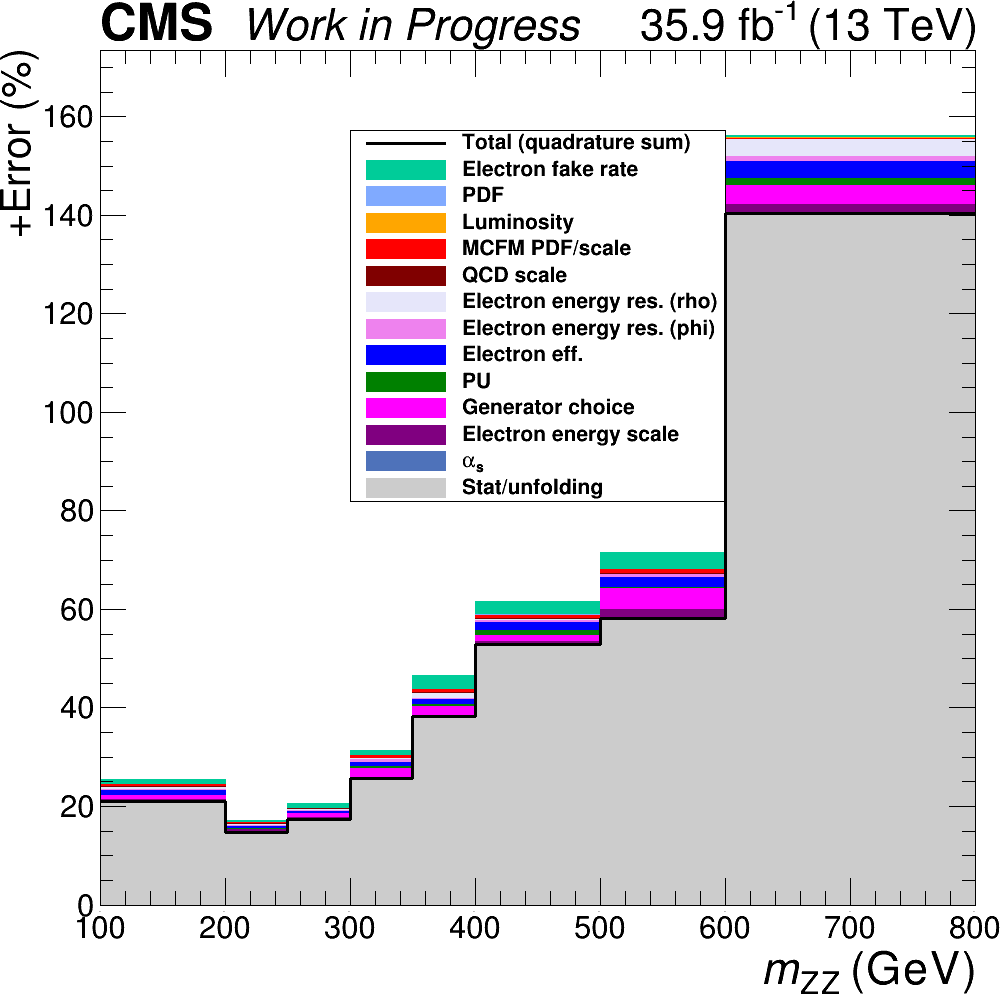
\includegraphics[width=0.45\textwidth]{methods/errUp_mass_eeee.png}
    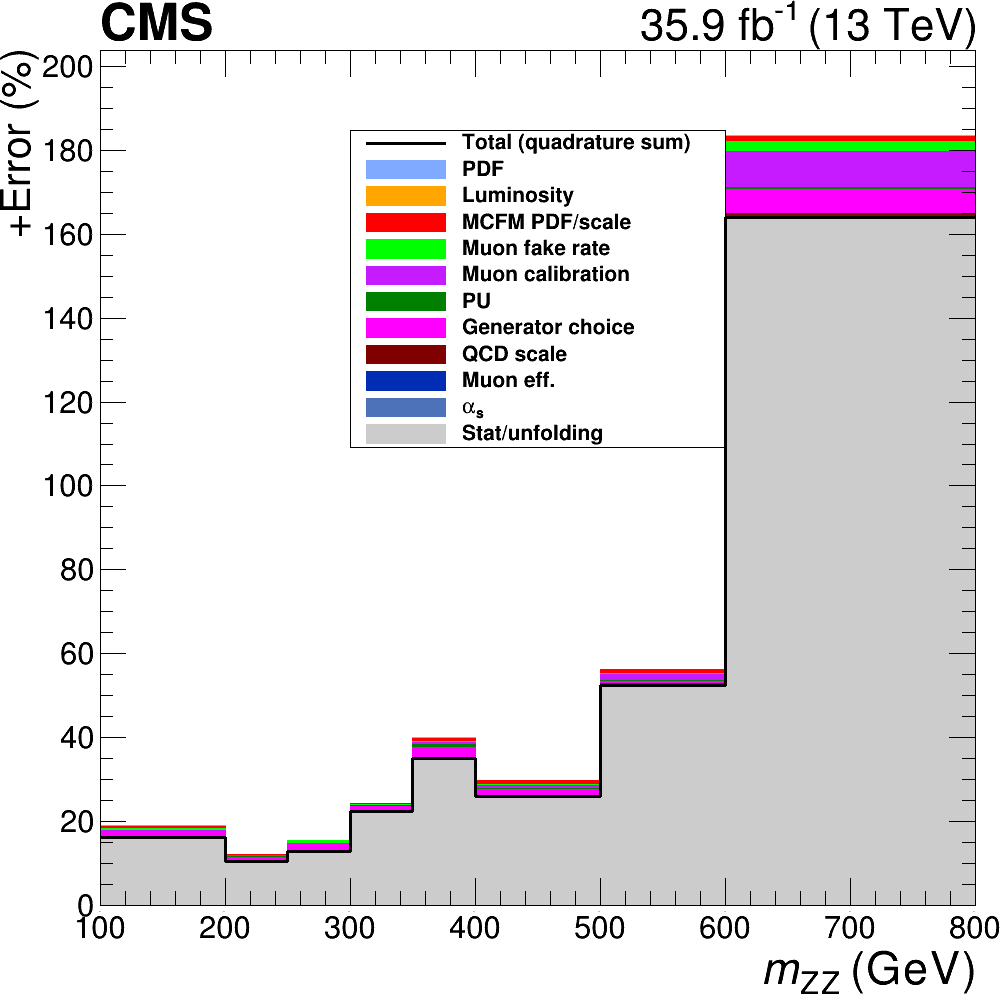
\includegraphics[width=0.45\textwidth]{methods/errUp_mass_mmmm.png}
    \caption[Differential cross section shape uncertainty sources]{
      Sources of positive shape uncertainties for the normalized differential cross section as a function of four-lepton mass, for $4\Pe$ events (left) and $4\Pm$ events (right).
      The grey histogram represents statistical errors, propagated through the unfolding procedure, and the histograms stacked on top of it represent various sources of systematic uncertainty.
      The thick black line represents the sum of all the uncertainties in quadrature.
      The systematic uncertainties are generally negligible compared to the statistical uncertainty.
      }\label{fig:unfold_unc}
  \end{center}
\end{figure}



\section{VBS Signal Extraction}\label{sec:vbsSearch}

The VBS signal search considers events passing the selections described in Section~\ref{sec:vbsSelection}.
The electroweak yield is insufficient to have sensitivity at 35.9\fbinv, even with further cut optimization, so a gradient-boosted decision tree (GBDT), implemented with the \textsc{Scikit-learn} package~\cite{scikit-learn}, is used to extract the signal.
Hyperparameters of the GBDT are optimized with a grid search.
Each Monte Carlo sample used in the VBS search (see Section~\ref{sec:samples}) is split into a ``training'' subsample, used to train the GBDT, and a ``test'' subsample used to evaluate its performance and make templates for use in the statistical analysis.
The GBDT performance is nearly the same for the test and training samples, a sign that the algorithm is not overtrained.

A number of observables have been proposed to discriminate VBS events from background~\cite{Zeppenfeld:54.6680}, of which $m_{\Pj\Pj}$ and $\Delta\eta_{\Pj\Pj}$ are the most powerful.
Other commonly-used variables include $m_{4\ell}$, $\eta^{\Pj_1} \times \eta^{\Pj_2}$, $\Delta\phi_{\PZ_1\PZ_2}$, and the so-called Zeppenfeld variables, defined as
\begin{equation}
  \eta^\ast_P = \eta_P - \frac{\eta_{\Pj_1} - \eta_{\Pj_2}}{2},
\end{equation}
where $P$ may stand for $\PZ_1$, $\PZ_2$, or $\Pj_3$, the highest-{\pt} untagged jet in the event.
In addition to these ``traditional'' quantities, several other groups of observables have been examined, including production angles, decay angles, measures of total hadronic activity in the event, properties of individual leptons and jets and of the $\PZ\PZ\Pj\Pj$ system, and a discriminator designed to distinguish jets originating from quarks and gluons~\cite{CMS:2013kfa}.
The hadronic activity and quark-gluon tagging variables have some discriminating power, but they differ significantly depending on the Monte Carlo generator used and were therefore considered too poorly-modeled to use.
New GBDTs were trained, each with the traditional observables and one other group of observables, and the groups that improved the GBDT discrimination power significantly were retained.
This procedure yielded 17 observables, including the hard process relative transverse momentum, defined as the ratio of the {\pt} of the $\PZ\PZ\Pj\Pj$ system to the scalar sum of the {\pt} of each object,
\begin{equation}
  \pt^\textit{rel. hard} = \frac{\pt^{\PZ\PZ\Pj\Pj}}{\sum_{\PZ_1,\PZ_2,\Pj_1,\Pj_2} \pt},
\end{equation}
and the dijet relative transverse momentum,
\begin{equation}
  \pt^{\textit{rel.}\ \Pj\Pj} = \frac{\pt^{\Pj\Pj}}{\sum_{\Pj_1,\Pj_2} \pt}.
\end{equation}

The list of observables was further optimized by retraining the GBDT once with each variable dropped and eliminating the one with the least discriminating power.
This pruning was repeated until seven observables remained, namely $m_{\Pj\Pj}$, $\Delta\eta_{\Pj\Pj}$, $m_{4\ell}$, $\eta^\ast_{\PZ_1}$, $\eta^\ast_{\PZ_2}$, $\pt^\textit{rel. hard}$, and $\pt^{\textit{rel.}\ \Pj\Pj}$.
The resulting GBDT performs only marginally worse ($0.2\sigma$ less expected significance on the VBS signal) than a version with all observables included, and is faster and easier to train, simpler, and less susceptible to biases and systematic uncertainties from mismodeling.

The signal and background yields are extracted from the GBDT output spectrum with a binned maximum likelihood fit to templates from the test Monte Carlo samples.
To obtain templates with better fit convergence properties, the GBDT output is mapped to the range $\left[0,1\right]$ with the logistic transformation
\begin{equation}
  x \rightarrow \frac{1}{1-e^{-x}}.
\end{equation}
This provides better separation between signal and background and allows uniform binning in the templates.



\section{Anomalous Gauge Coupling Searches}\label{sec:aGCSearch}

The new physics represented by aGCs would generally manifest as an increase in events with high invariant mass, so it is natural to use the shape of the $m_{4\ell}$ distribution for the search.
For the aTGC search, the doubly on-shell {\ZZ} selection is used, while the aQGC search is performed with the $\PZ\PZ\Pj\Pj$ selection described in Section~\ref{sec:vbsSelection}.

Monte Carlo samples with nonzero aTGCs are generated at grids of points in the $f_4^\PZ$-$f_4^\Pa$ and $f_5^\PZ$-$f_5^\Pa$ planes.
In each bin of the $m_{4\ell}$ distribution, the yields at the various working points are fit to a function of the form
\begin{equation}
  y\left(f^\PZ,f^\Pa\right) = x_0 + x_1 f^\PZ + x_2 f^\Pa + x_3 f^\PZ f^\Pa + x_4 \left(f^\PZ\right)^2 + x_5 \left(f^\Pa\right)^2
\end{equation}
where $y\left(f^\PZ,f^\Pa\right)$ is the yield in the bin, $f^\PV$ can be $f^\PZ_4$ and $f^\Pa_4$ or $f^\PZ_5$ and $f^\Pa_5$, and $x_i$ are the parameters to be fit.

A similar procedure is performed for the aQGC search.
Rather than simulating a full sample for each working point, which is computationally expensive, events from \textsc{MadGraph5\_aMC} produced at LO are used to obtain samples for nonzero values of $f_\text{T0} / \Lambda^4$, $f_\text{T1} / \Lambda^4$, $f_\text{T2} / \Lambda^4$, $f_\text{T8} / \Lambda^4$, and $f_\text{T9} / \Lambda^4$ by matrix element reweighting~\cite{Alwall:2014hca}.
The yields in each $m_{4\ell}$ bin are fit to parabolas as a function of the five aQGC parameters separately.

A binned profile likelihood method~\cite{Olive:2016xmw} is used to derive the limits.
Systematic uncertainties are taken into account by varying the number of signal and background events within their uncertainties.
Exclusion limits are found by comparing the p-values of the signal hypothesis and the background only hypothesis
\begin{equation}
  CL_s = \frac{p_{s+b}}{1-p_b}
\end{equation}
to set thresholds.
Further details on the method can be found in Ref.~\cite{Cowan:2010js}.
The software for setting limits, implemented with \textsc{RooStats}, has been validated and used extensively by the CMS and ATLAS collaborations~\cite{CMS:2016nxa}.

%!TEX root = ../nwoods_thesis.tex

\chapter{Results}\label{ch:results}

A number of measurements and analyses fall under the umbrella of four-lepton physics, and results presented in this thesis were originally made public in several journal articles and Physics Analysis Summary documents released by the CMS collaboration.
The first CMS measurement of the {\ZZ} inclusive cross section at {13\TeV} used roughly half the 2015 dataset ({1.34\fbinv}) and was made public in Ref.~\cite{CMS:2015fnj} in December 2015 as one of the first measurements done on {13\TeV} collision data.
That analysis was expanded to use the whole {2.6\fbinv} collected in 2015, and to include the {\Zfourl} branching fraction measurement, as reported in Ref.~\cite{Khachatryan:2016txa}, submitted in July 2016 and published the following December.
With the full 2016 dataset, the {\ZZ} cross section and {\Zfourl} branching ratio were measured again to greater precision in Ref.~\cite{CMS:2017ruh}, which also included differential cross section measurements and aTGC limits, made public in March 2017.
A new paper including these measurements~\cite{Sirunyan:2017zjc} also includes a combination of the 2015 and 2016 inclusive cross section measurements.
Differential cross sections with respect to jet-related observables, and searches for EWK {\ZZ} production and aTGCs, were reported in May 2017 in Ref.~\cite{CMS:2017dyw}, with a paper on only the VBS and aQGC searches following~\cite{Sirunyan:2017fvv}.
The Higgs boson was studied in the four-lepton final state in Refs.~\cite{CMS:2016rqf,CMS:2016ilx,Sirunyan:2017exp}.
In the following, results for each topic are only shown for 2016 data, which significantly exceed the accuracy of the results from 2015 data.



\section{Four-Lepton Yields and Inclusive Cross Sections}


\subsection{Full Spectrum}

The full four-lepton invariant mass spectrum is shown in Fig.~\ref{fig:mass_full}.
The single-{\PZ} resonance can be seen below {100\GeV}, the Higgs resonance is visible---though it is not sharply resolved with this binning---in the {\Zgs} region below $2m_\PZ$, where doubly resonant {\ZZ} continuum production begins.
The dilepton invariant mass spectrum is shown for both {\Zgs} candidates in Fig.~\ref{fig:zMass_full} and for the {\Zgs} candidate closest to the nominal {\PZ} boson mass ($\PZ_1$) in Fig.~\ref{fig:z1Mass_full}.
Figure~\ref{fig:mZ2VsmZ1_full} shows $m_{\PZ_2}$ plotted against $m_{\PZ_1}$ for data events representative of all four-lepton production.
Clusters of events with zero ({\Zfourl} and nonresonant $\Pa^\ast \Pa^\ast$ production), one ($\PH \to \PZ\PZ^\ast$ and nonresonant $\PZ\Pa^\ast$ production), and two (nonresonant {\ZZ} production) on-shell {\PZ} bosons can be clearly seen.

\begin{figure}[htbp]
  \begin{center}
    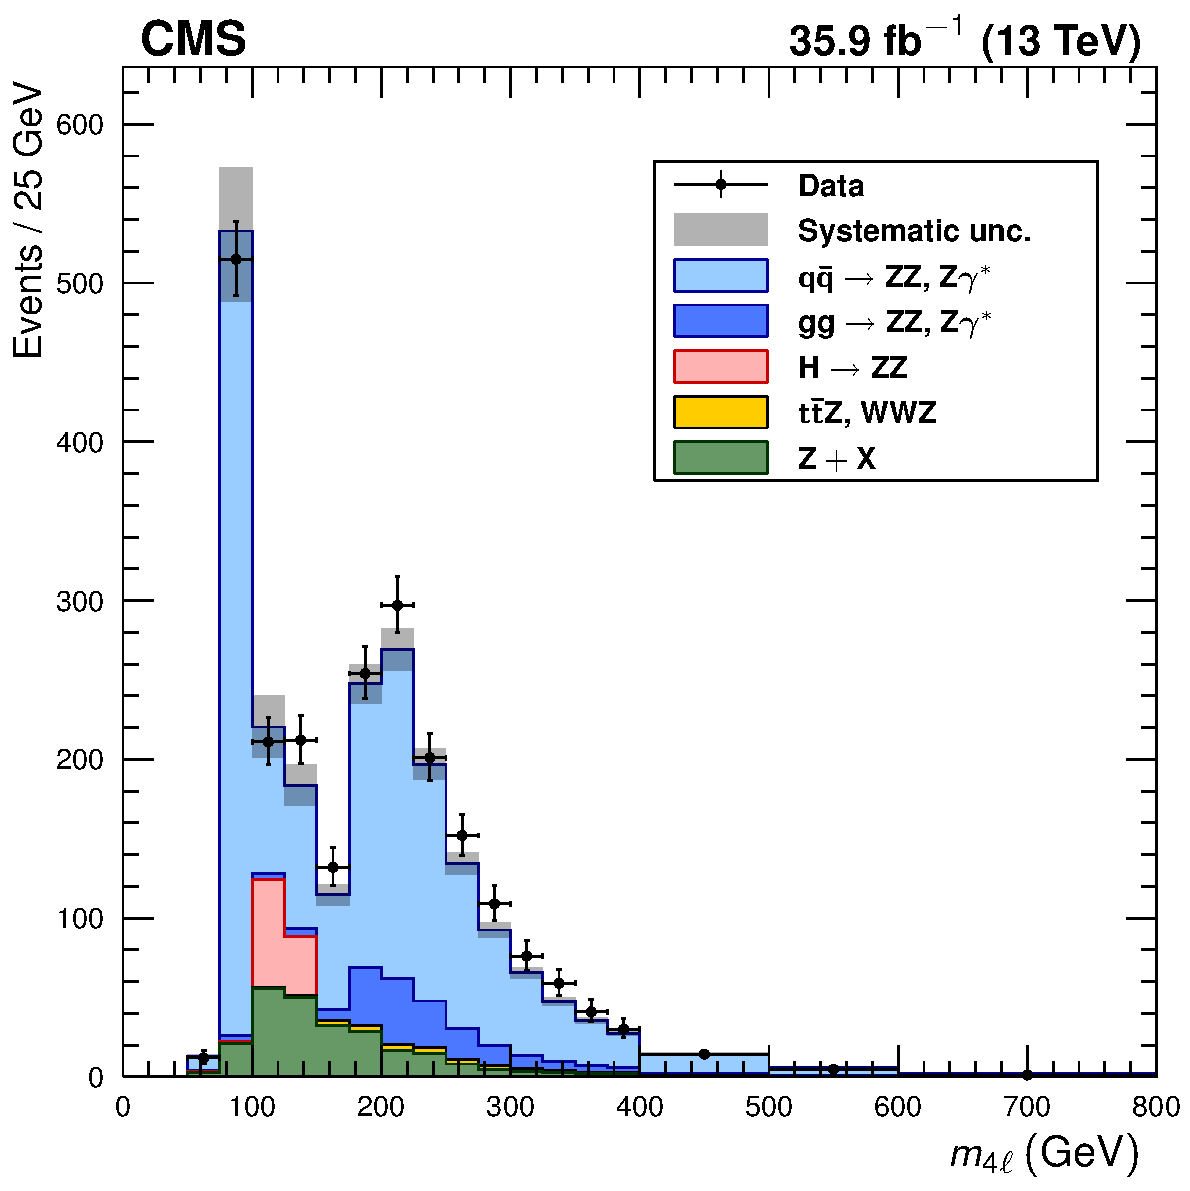
\includegraphics[width=0.75\textwidth]{results/zzMass.pdf}
    \caption[Full four-lepton mass spectrum]{
        Distribution of the four-lepton invariant mass $m_{4\ell}$ of all events in the full spectrum selection.
        Points represent data, with statistical uncertainty bars.
        The stack of filled histograms represents the SM signal prediction and background estimate, with a grey band showing the sum in quadrature of the statistical and systematic uncertainties on the total expected yield.
      }\label{fig:mass_full}
  \end{center}
\end{figure}

\begin{figure}[htbp]
  \begin{center}
    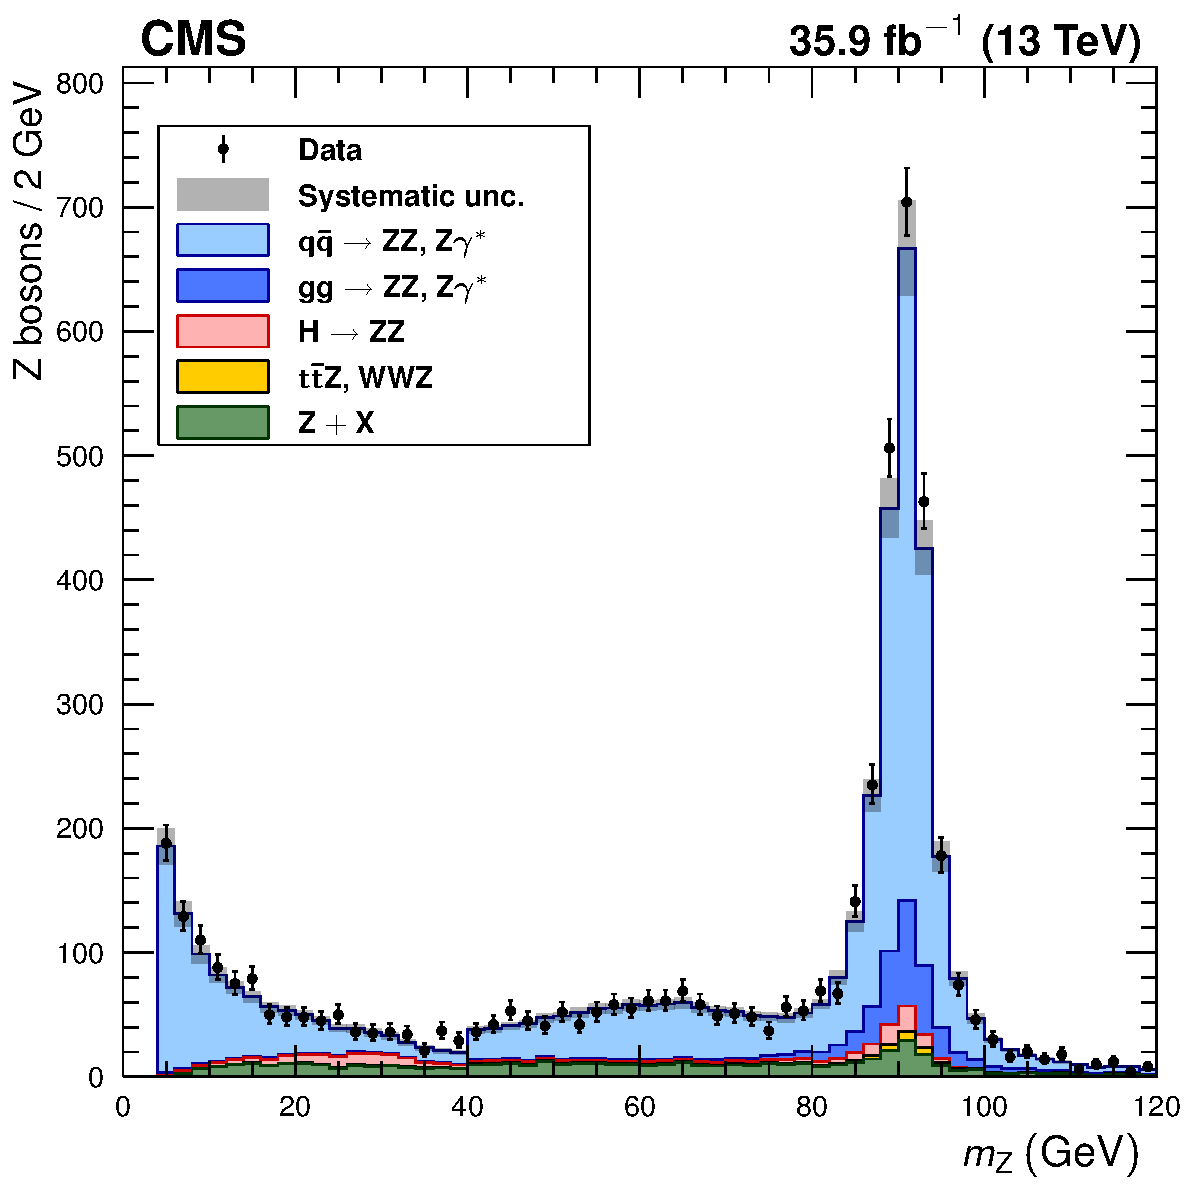
\includegraphics[width=0.75\textwidth]{results/zMass.pdf}
    \caption[Mass of all {\Zgs} candidates in the full spectrum selection]{
        Distribution of the dilepton invariant mass of {\Zgs} candidates in all events in the full spectrum selection, regardless of whether the lepton pair is labeled $\PZ_1$ or $\PZ_2$.
        Points represent data, with statistical uncertainty bars.
        The stack of filled histograms represents the SM signal prediction and background estimate, with a grey band showing the sum in quadrature of the statistical and systematic uncertainties on the total expected yield.
      }\label{fig:zMass_full}
  \end{center}
\end{figure}

\begin{figure}[htbp]
  \begin{center}
    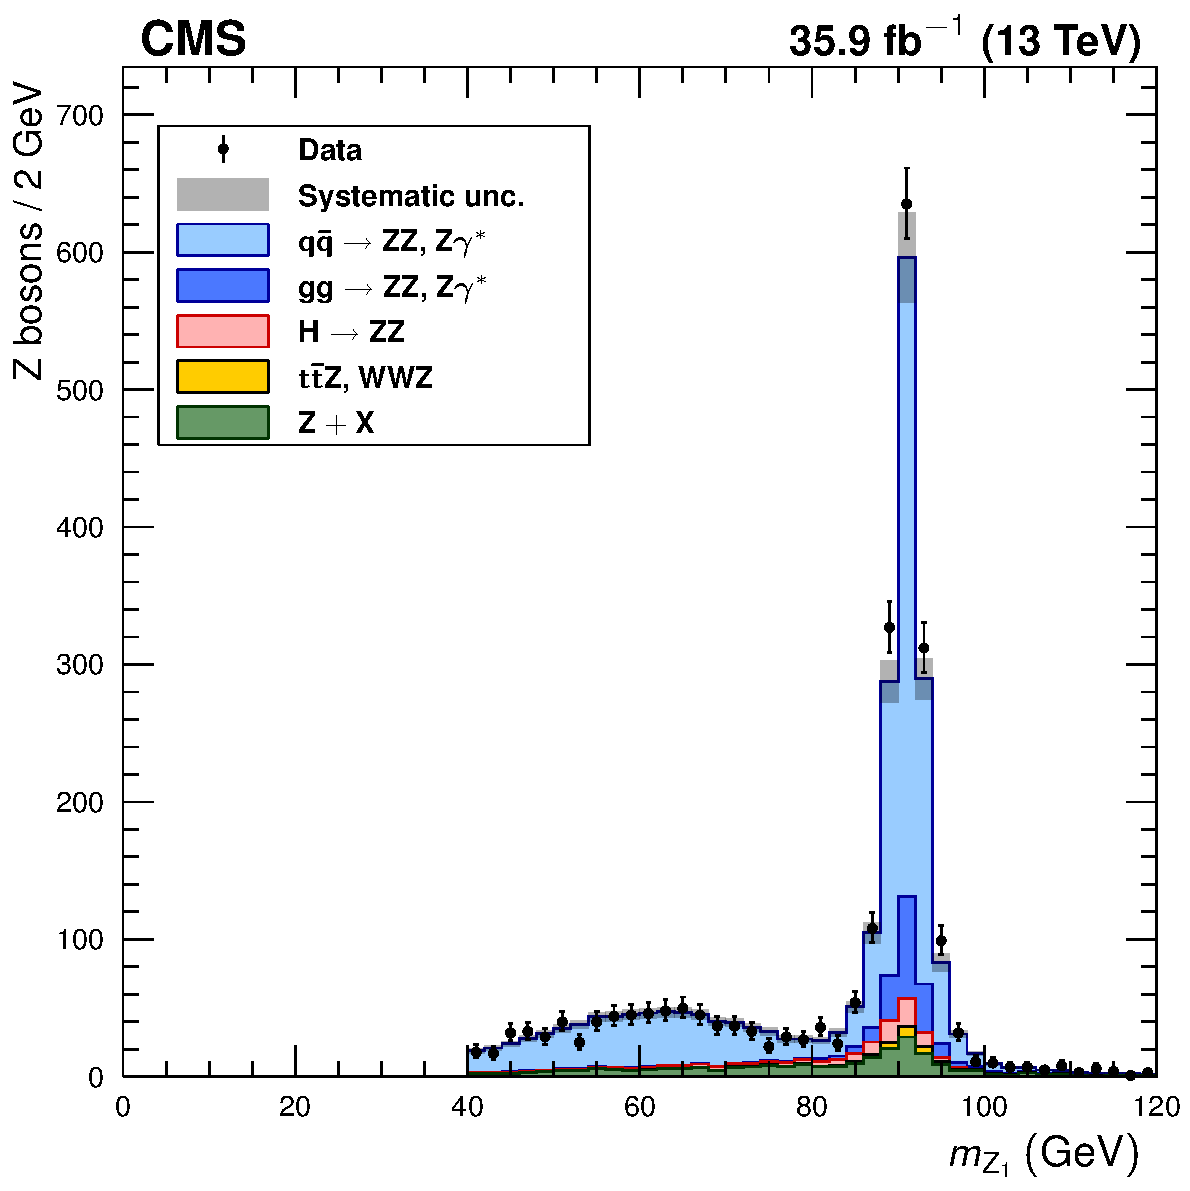
\includegraphics[width=0.75\textwidth]{results/z1Mass.pdf}
    \caption[Mass of $\PZ_1$ candidates in the full spectrum selection]{
        Distribution of the dilepton invariant mass of $\PZ_1$, the {\Zgs} candidate in each event closest to the nominal $m_\PZ$, in the full spectrum selection.
        Points represent data, with statistical uncertainty bars.
        The stack of filled histograms represents the SM signal prediction and background estimate, with a grey band showing the sum in quadrature of the statistical and systematic uncertainties on the total expected yield.
      }\label{fig:z1Mass_full}
  \end{center}
\end{figure}

\begin{figure}[htbp]
  \begin{center}
    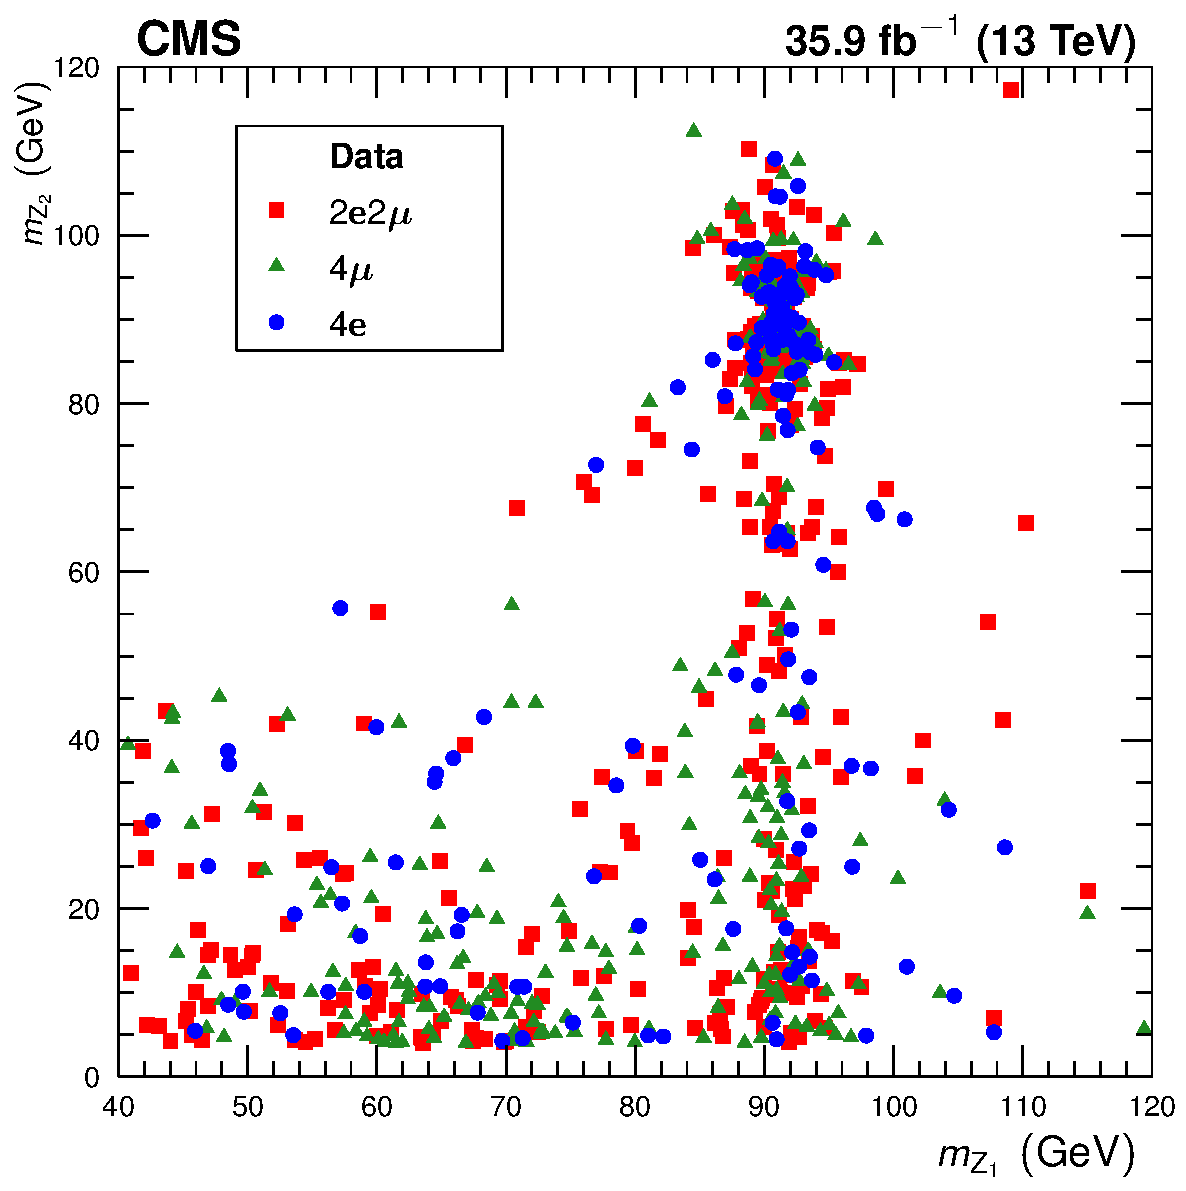
\includegraphics[width=0.75\textwidth]{results/mZ2VsmZ1_full.pdf}
    \caption[Scatter plot of $m_{\PZ_2}$ vs.\ $m_{\PZ_1}$ for data events in the full spectrum selection]{
        The reconstructed $m_{\PZ_2}$ plotted against the reconstructed $m_{\PZ_1}$ for data events in the full spectrum selection, with distinctive markers for each final state.
        For readability, only every fourth event is drawn.
        Clusters of events from different production modes are visible, as discussed in the text.
      }\label{fig:mZ2VsmZ1_full}
  \end{center}
\end{figure}


\subsection[\texorpdfstring{$\mathrm{Z} \to 4\ell$}{Z to 4l} Resonance]{$\mathbf{Z} \to \mathbf{4\ell}$ Resonance}

Expected and observed yields for events satisfying the {\Zfourl} selection criteria ($80 < m_{4\ell} < 100\GeV$) are shown in Table~\ref{tab:results_z4l}.
The invariant mass distribution of these events is shown in Fig.~\ref{fig:mass_z4l}.
Figure~\ref{fig:mZ2VsmZ1_z4l} shows $m_{\PZ_2}$ plotted against $m_{\PZ_1}$ for all data events consistent with {\Zfourl} production.
Predictions from Monte Carlo samples generally agree well with the data, allowing us to measure  the {\Zfourl} cross section and branching fraction.

\begin{table}[htbp]
  \begin{center}
    \caption[Expected and observed yields for {\Zfourl} production.]{
      Observed and expected yields of {\Zfourl} events, including expected background yields, shown for each final state and summed to the total.
      Uncertainties are statistical, then systematic, not including the integrated luminosity uncertainty.
    }\label{tab:results_z4l}
    \begin{tabular}{ccccc}
      \toprule
      Final & Expected     &  Background   & Total     & Observed \\
      state & $N_{4\ell}$  &               & expected  &          \\
      \midrule
      \midrule
      $4\Pm$       & $ 224 \pm 1 \pm 16   $  & $ 7 \pm 1 \pm 2    $  & $ 231 \pm 2 \pm 17   $  & $ 225 $  \\
      $2\Pe 2\Pm$  & $ 207 \pm 1 \pm 14   $  & $ 9 \pm 1 \pm 2    $  & $ 216 \pm 2 \pm 14   $  & $ 206 $  \\
      $4\Pe$       & $ 68 \pm 1 \pm 8     $  & $ 4 \pm 1 \pm 2    $  & $ 72 \pm 1 \pm 8     $  & $ 78  $  \\
      \midrule
      Total        & $ 499  \pm 2  \pm 32 $  & $ 19  \pm 2  \pm 5 $  & $ 518  \pm 3  \pm 33 $  & $ 509 $  \\
      \bottomrule
    \end{tabular}
  \end{center}
\end{table}

\begin{figure}[htbp]
  \begin{center}
    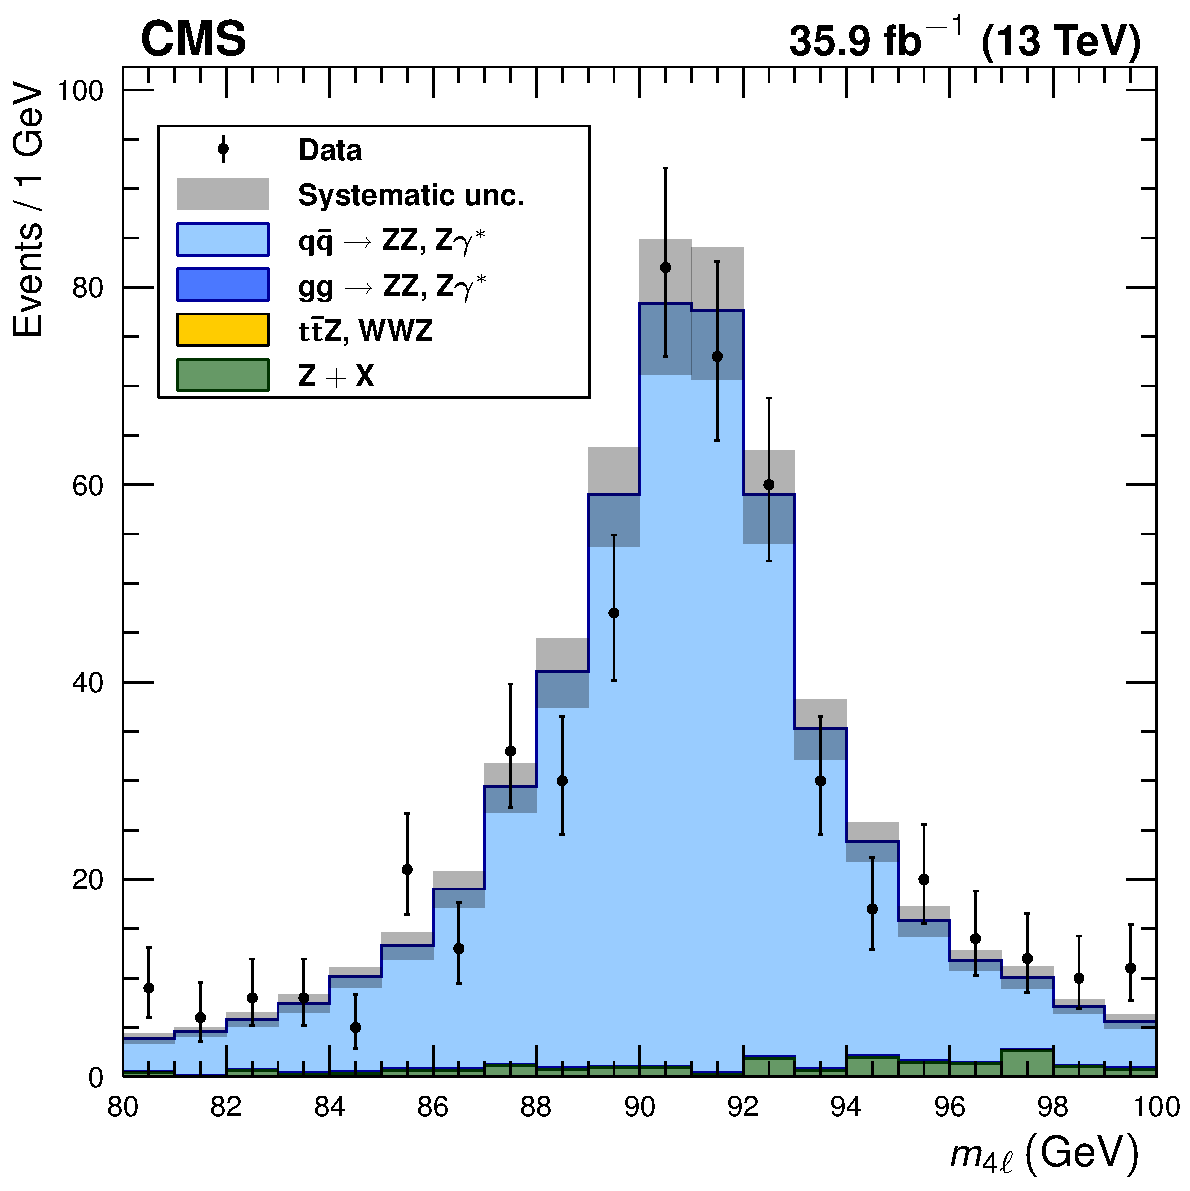
\includegraphics[width=0.75\textwidth]{results/z4lzzMass.pdf}
    \caption[Four-lepton mass in the {\Zfourl} selection]{
        Distribution of the four-lepton invariant mass $m_{4\ell}$ of all events in the mass range $80 < m_{4\ell} < 100\GeV$, the {\Zfourl} selection.
        Points represent data, with statistical uncertainty bars.
        The stack of filled histograms represents the SM signal prediction and background estimate, with a grey band showing the sum in quadrature of the statistical and systematic uncertainties on the total expected yield.
      }\label{fig:mass_z4l}
  \end{center}
\end{figure}

\begin{figure}[htbp]
  \begin{center}
    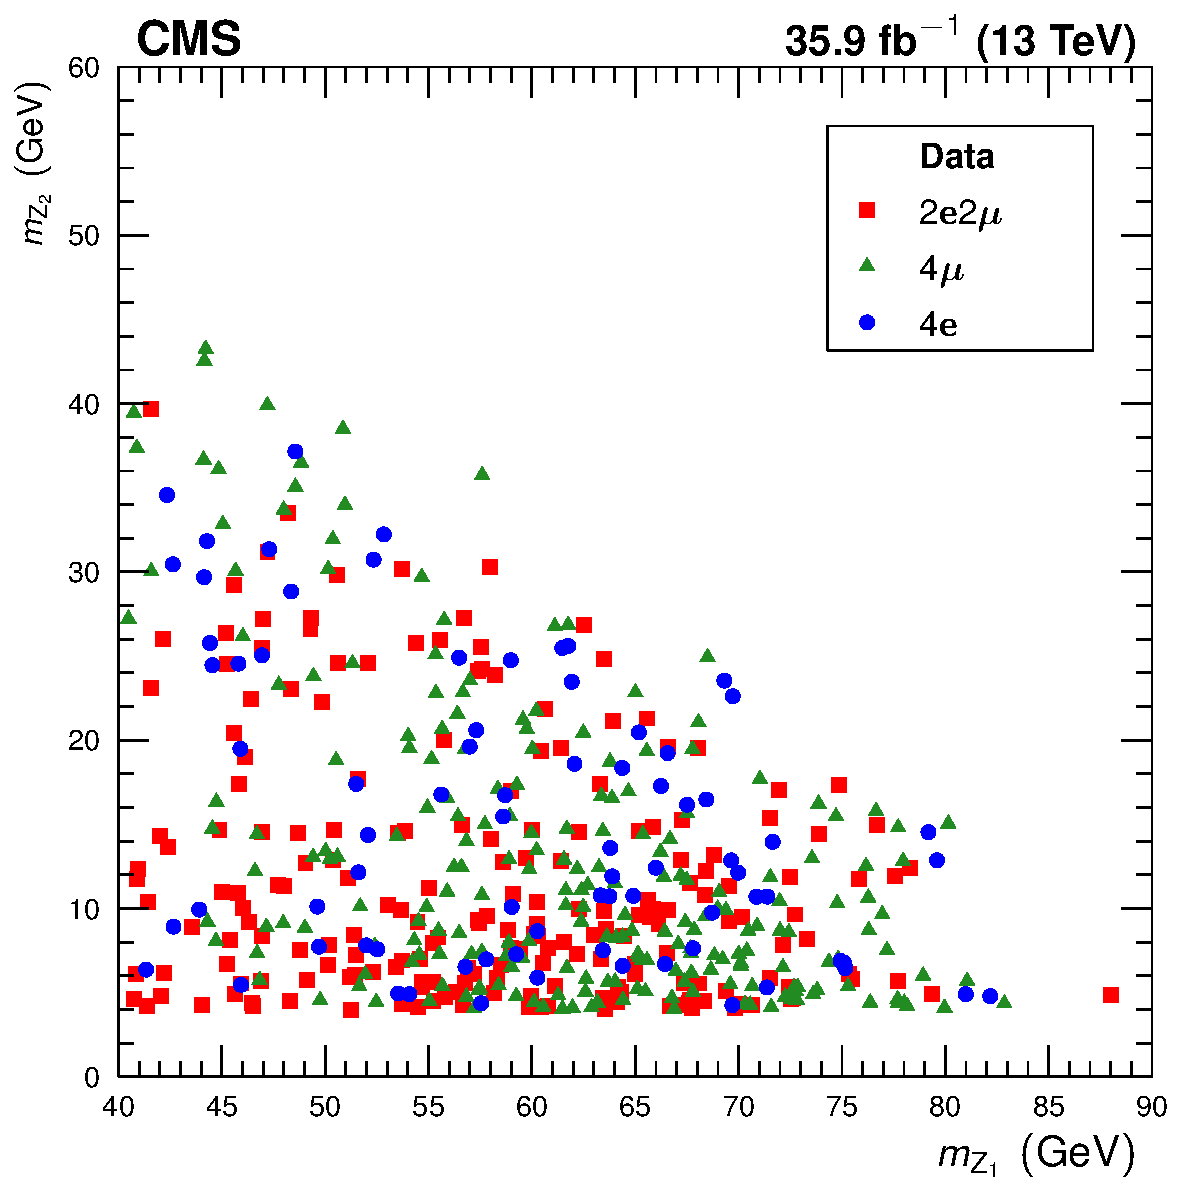
\includegraphics[width=0.75\textwidth]{results/mZ2VsmZ1_z4l.pdf}
    \caption[Scatter plot of $m_{\PZ_2}$ vs.\ $m_{\PZ_1}$ for data events in the {\Zfourl} selection]{
        The reconstructed $m_{\PZ_2}$ plotted against the reconstructed $m_{\PZ_1}$ for all data events with $80 < m_{4\ell} < 100\GeV$, with distinctive markers for each final state.
      }\label{fig:mZ2VsmZ1_z4l}
  \end{center}
\end{figure}


The signal strength in the {\Zfourl} selection is
\begin{equation}
  \mu = 0.980 _{-0.044}^{+0.046} \stat _{-0.059}^{+0.065} \syst \pm 0.025 \lum,
\end{equation}
yielding a fiducial cross section
\begin{equation}
  \sigma_\text{fid}\left(\pp \to \PZ \to 4\ell\right) = 31.2 _{-1.4}^{+1.5} \stat _{-1.9}^{+2.1} \syst \pm 0.8 \lum \unit{fb}.
\end{equation}
This is scaled by an acceptance correction factor $\mathcal{A} = 0.125 \pm 0.002$, estimated with {\POWHEG}~v2.0, to the total {\Zfourl} cross section times branching ratio,
\begin{equation}
  \sigma(\pp \to \PZ) \times \mathcal{B}(\PZ \to 4\ell) = 249 \pm 8 \stat ^{+9}_{-8} \syst \pm 4 \thy \pm 6 \lum \unit{fb}.
\end{equation}

Equation~(\ref{eq:brCalc}) is used to calculate the branching fraction.
The {\PZ} cross section times dilepton branching ratio is calculated with {\FEWZ}~v2.0~\cite{Gavin:2010az} at NNLO in QCD to be $\sigma(\PZ \to 2\ell) = 1870 ^{+50}_{-40}\unit{pb}$.
The {\PZ} mass window correction factor is calculated with {\POWHEG} and found to be $\mathcal{C}^{\text{60--120}}_{\text{80--100}} = 0.926 \pm 0.001$.
Its uncertainty includes scale and PDF variations~\cite{Butterworth:2015oua}.
The nominal {\PZ} to dilepton branching fraction is $\mathcal{B}\left( \PZ \to 2\ell \right) = 0.03366$~\cite{Olive:2016xmw}.
The four-lepton branching fraction is measured to be
\begin{equation}
  \mathcal{B}\left(\Zfourl\right) = 4.8 \pm 0.2 \stat \pm 0.2 \syst \pm 0.1 \thy \pm 0.1 \lum \times 10^{-6}.
\end{equation}
This value is consistent with the theoretical value of $4.6 \times 10^{-6}$, calculated with {\MGAMC}~v2.3.3, and with previous measurements from CMS and ATLAS~\cite{CMS:2012bw,Khachatryan:2016txa,Aad:2014wra}, which had uncertainties 2--4 times larger.


\subsection{Higgs Resonance}

Figure~\ref{fig:mass_hzz} shows the four-lepton invariant mass around the Higgs resonance, which can be clearly seen above the SM continuum background, for events passing the Higgs selection ($m_{\PZ_2} > 12\GeV$, $\text{SIP}_\text{3D} < 4$ for all leptons).
Table~\ref{tab:results_hzz} shows the observed and expected yields in the mass range $118 < m_{4\ell} < 130\GeV$.
Here, SM continuum production---considered signal in all other parts of this analysis---is considered background.
Figures~\ref{fig:z1Mass_hzz}--\ref{fig:mZ2VsmZ1_hzz} show the $\PZ_1$ mass, the $\PZ_2$ mass, and the scatter plot of $m_{\PZ_2}$ against $m_{\PZ_1}$, for events in the same four-lepton mass region around the Higgs resonance.
Agreement between predictions and data is again good, allowing measurements of Higgs boson properties, couplings, and production rates.
These are beyond the scope of this thesis, but were reported in Ref.~\cite{Sirunyan:2017exp}.

\begin{figure}[htbp]
  \begin{center}
    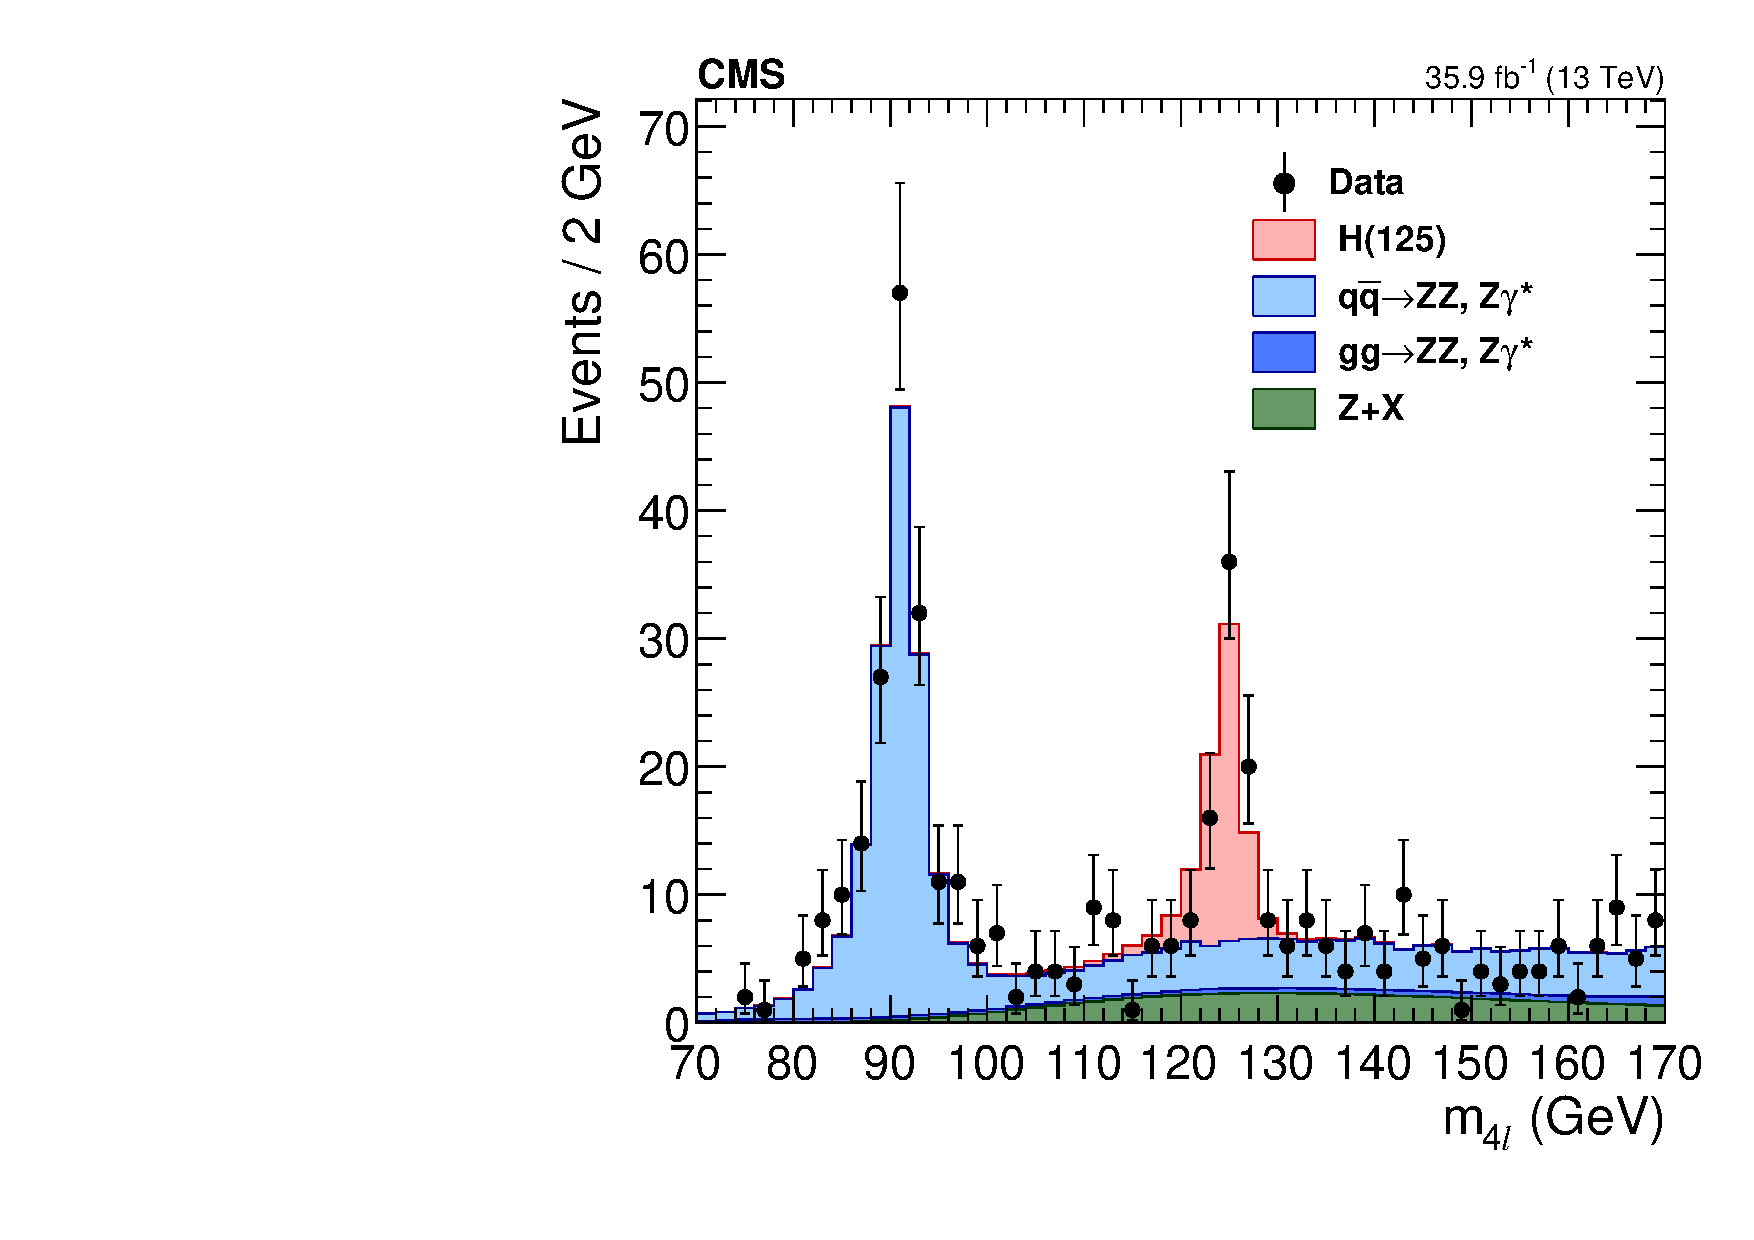
\includegraphics[width=0.75\textwidth]{results/hzzMass.pdf}
    \caption[Four-lepton mass spectrum around the Higgs resonance]{
        Distribution of the four-lepton invariant mass $m_{4\ell}$ for events in the Higgs selection.
        Points represent data, with statistical uncertainty bars.
        The stack of filled histograms represents the signal and SM background predictions and the reducible background estimate.
      }\label{fig:mass_hzz}
  \end{center}
\end{figure}

\begin{table}[htbp]
  \begin{center}
    \caption[Expected and observed yields for Higgs boson production.]{
      Observed and expected yields of $\PH \to \PZ\PZ^\ast \to 4\ell$ events, including expected background yields, for events passing the Higgs selection in the mass range $118 < m_{4\ell} < 130\GeV$, shown for each final state and summed to the total.
      Uncertainties are statistical and systematic combined.
    }\label{tab:results_hzz}
    \begin{tabular}{cccccc}
      \toprule
      Final & Expected   &  SM continuum & $\PZ + \PX$  & Total     & Observed \\
      state & $N_\PH$    &  background   &              & expected  &          \\
      \midrule
      \midrule
      $4\Pm$       & $ 21.6 \pm 1.9   $  & $ 9.4  ^{+0.6}_{-0.7}   $  & $ 4.7  ^{+2.0}_{-1.8}  $  & $ 35.8 \pm 2.9        $  & $ 34 $ \\
      $2\Pe 2\Pm$  & $ 26.5 \pm 2.3   $  & $ 11.0 ^{+0.7}_{-0.8}   $  & $ 6.9  ^{+3.1}_{-2.9}  $  & $ 44.4 ^{+3.7}_{-3.6} $  & $ 41 $ \\
      $4\Pe$       & $ 10.2 \pm 1.1   $  & $ 3.6  \pm 0.3          $  & $ 1.9  ^{+0.8}_{-1.0}  $  & $ 15.8 \pm 1.6        $  & $ 19 $ \\
      \midrule
      Total        & $ 58.3 \pm 5.0   $  & $ 24.1 ^{+1.5}_{-1.6}   $  & $ 13.5 ^{+3.7}_{-3.5}  $  & $ 96.0 \pm 6.7        $  & $ 94 $ \\
      \bottomrule
    \end{tabular}
  \end{center}
\end{table}

\begin{figure}[htbp]
  \begin{center}
    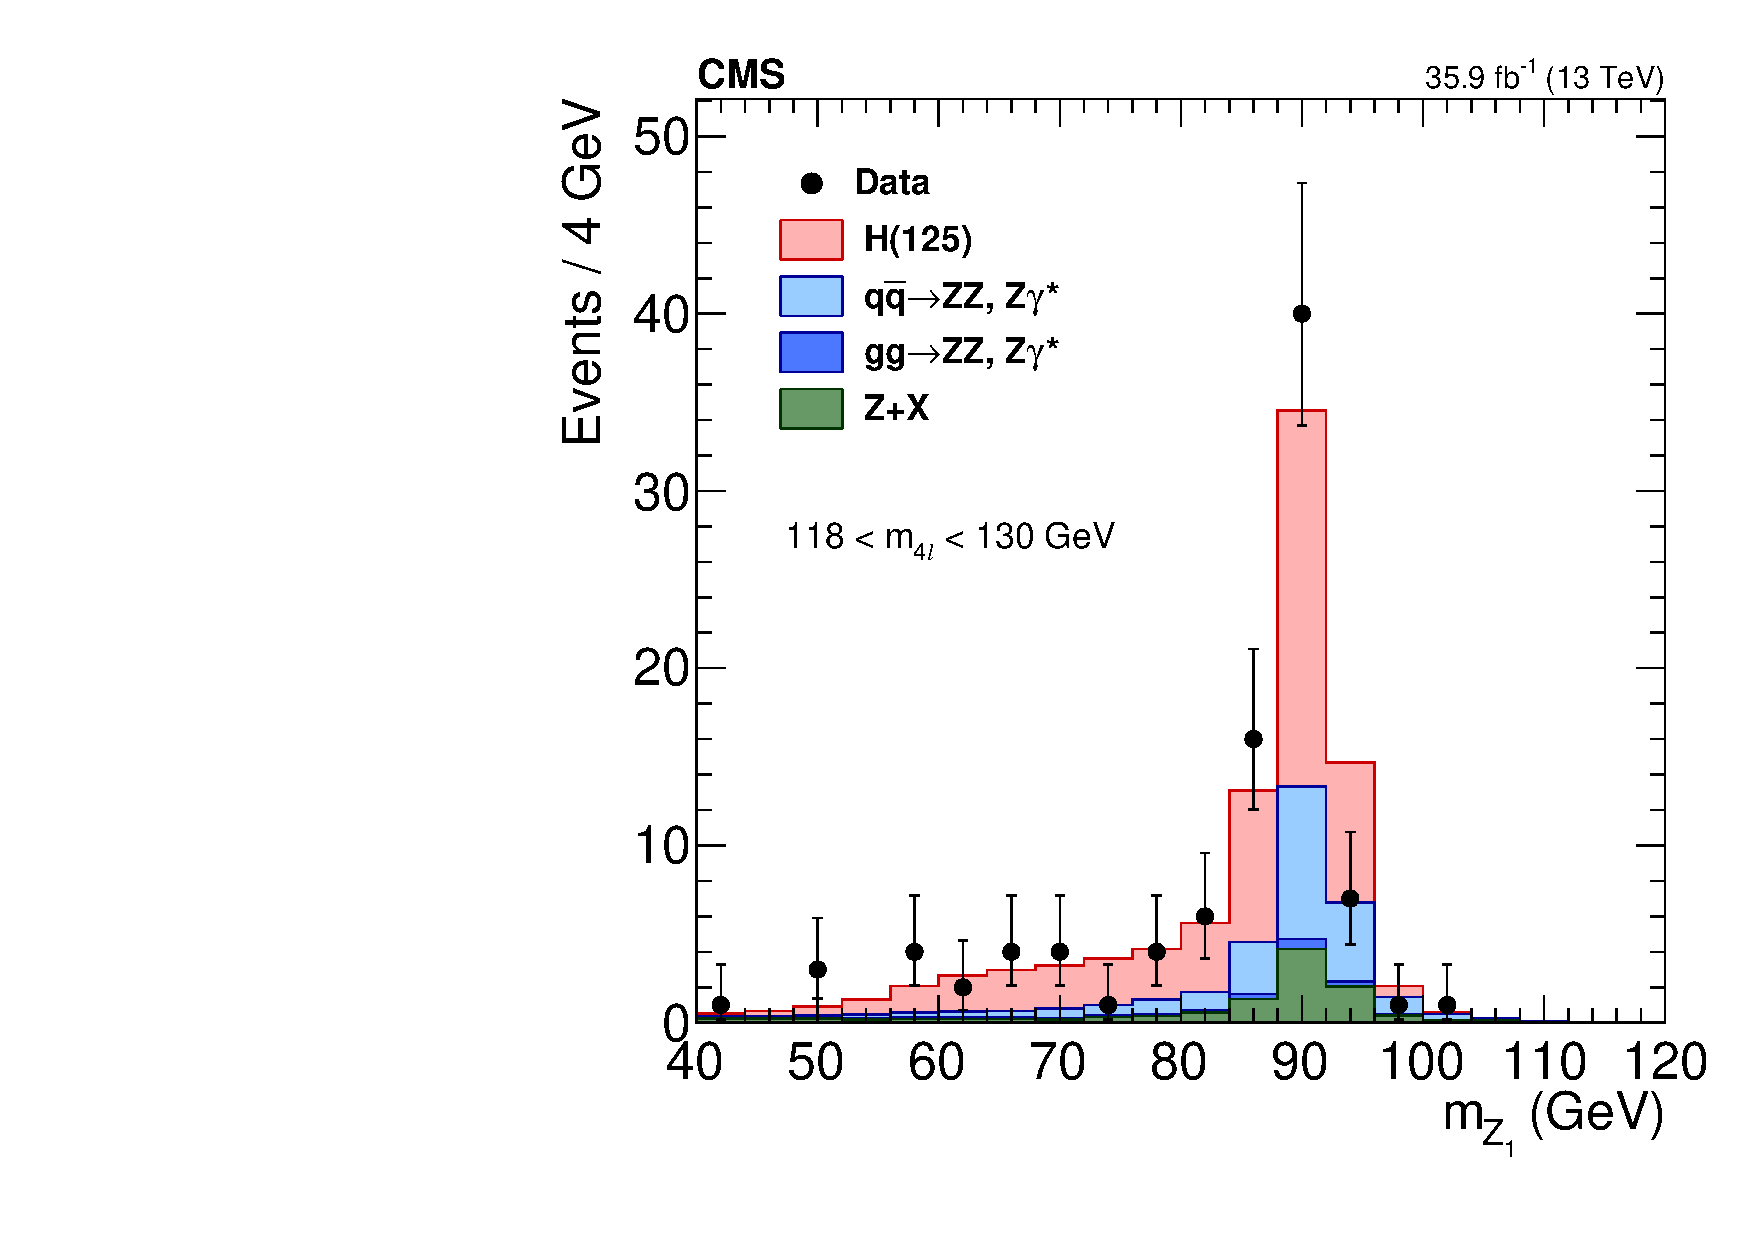
\includegraphics[width=0.75\textwidth]{results/hzzz1Mass.pdf}
    \caption[Mass of $\PZ_1$ candidates in events near the Higgs resonance]{
        Distribution of the dilepton invariant mass of $\PZ_1$, the dilepton candidate in each event closest to the nominal $m_\PZ$, in events in the Higgs selection with $118 < m_{4\ell} < 130\GeV$.
        Points represent data, with statistical uncertainty bars.
        The stack of filled histograms represents the signal and SM background predictions and the reducible background estimate.
      }\label{fig:z1Mass_hzz}
  \end{center}
\end{figure}

\begin{figure}[htbp]
  \begin{center}
    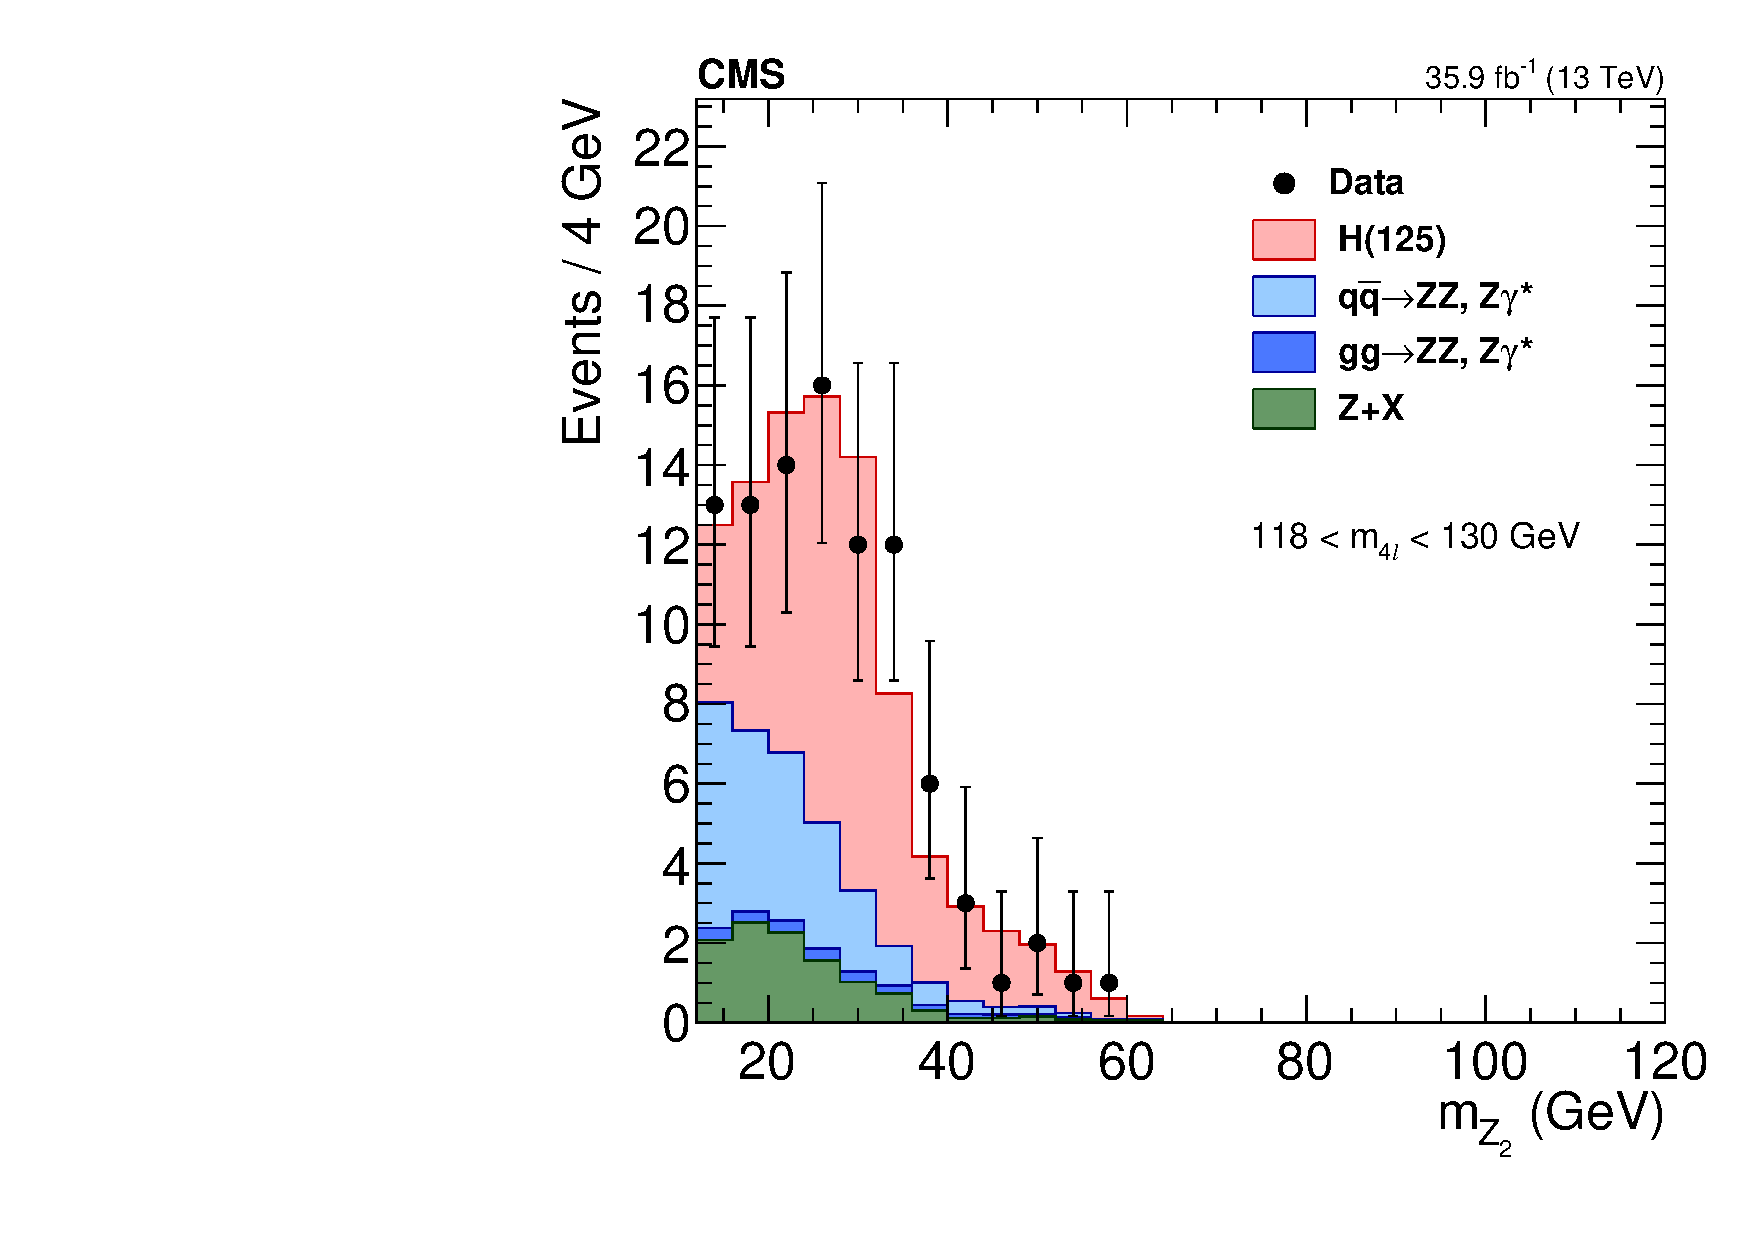
\includegraphics[width=0.75\textwidth]{results/hzzz2Mass.pdf}
    \caption[Mass of $\PZ_2$ candidates in events near the Higgs resonance]{
        Distribution of the dilepton invariant mass of $\PZ_2$, the dilepton candidate in each event farther from the nominal $m_\PZ$, in events in the Higgs selection with $118 < m_{4\ell} < 130\GeV$.
        Points represent data, with statistical uncertainty bars.
        The stack of filled histograms represents the signal and SM background predictions and the reducible background estimate.
      }\label{fig:z2Mass_hzz}
  \end{center}
\end{figure}

\begin{figure}[htbp]
  \begin{center}
    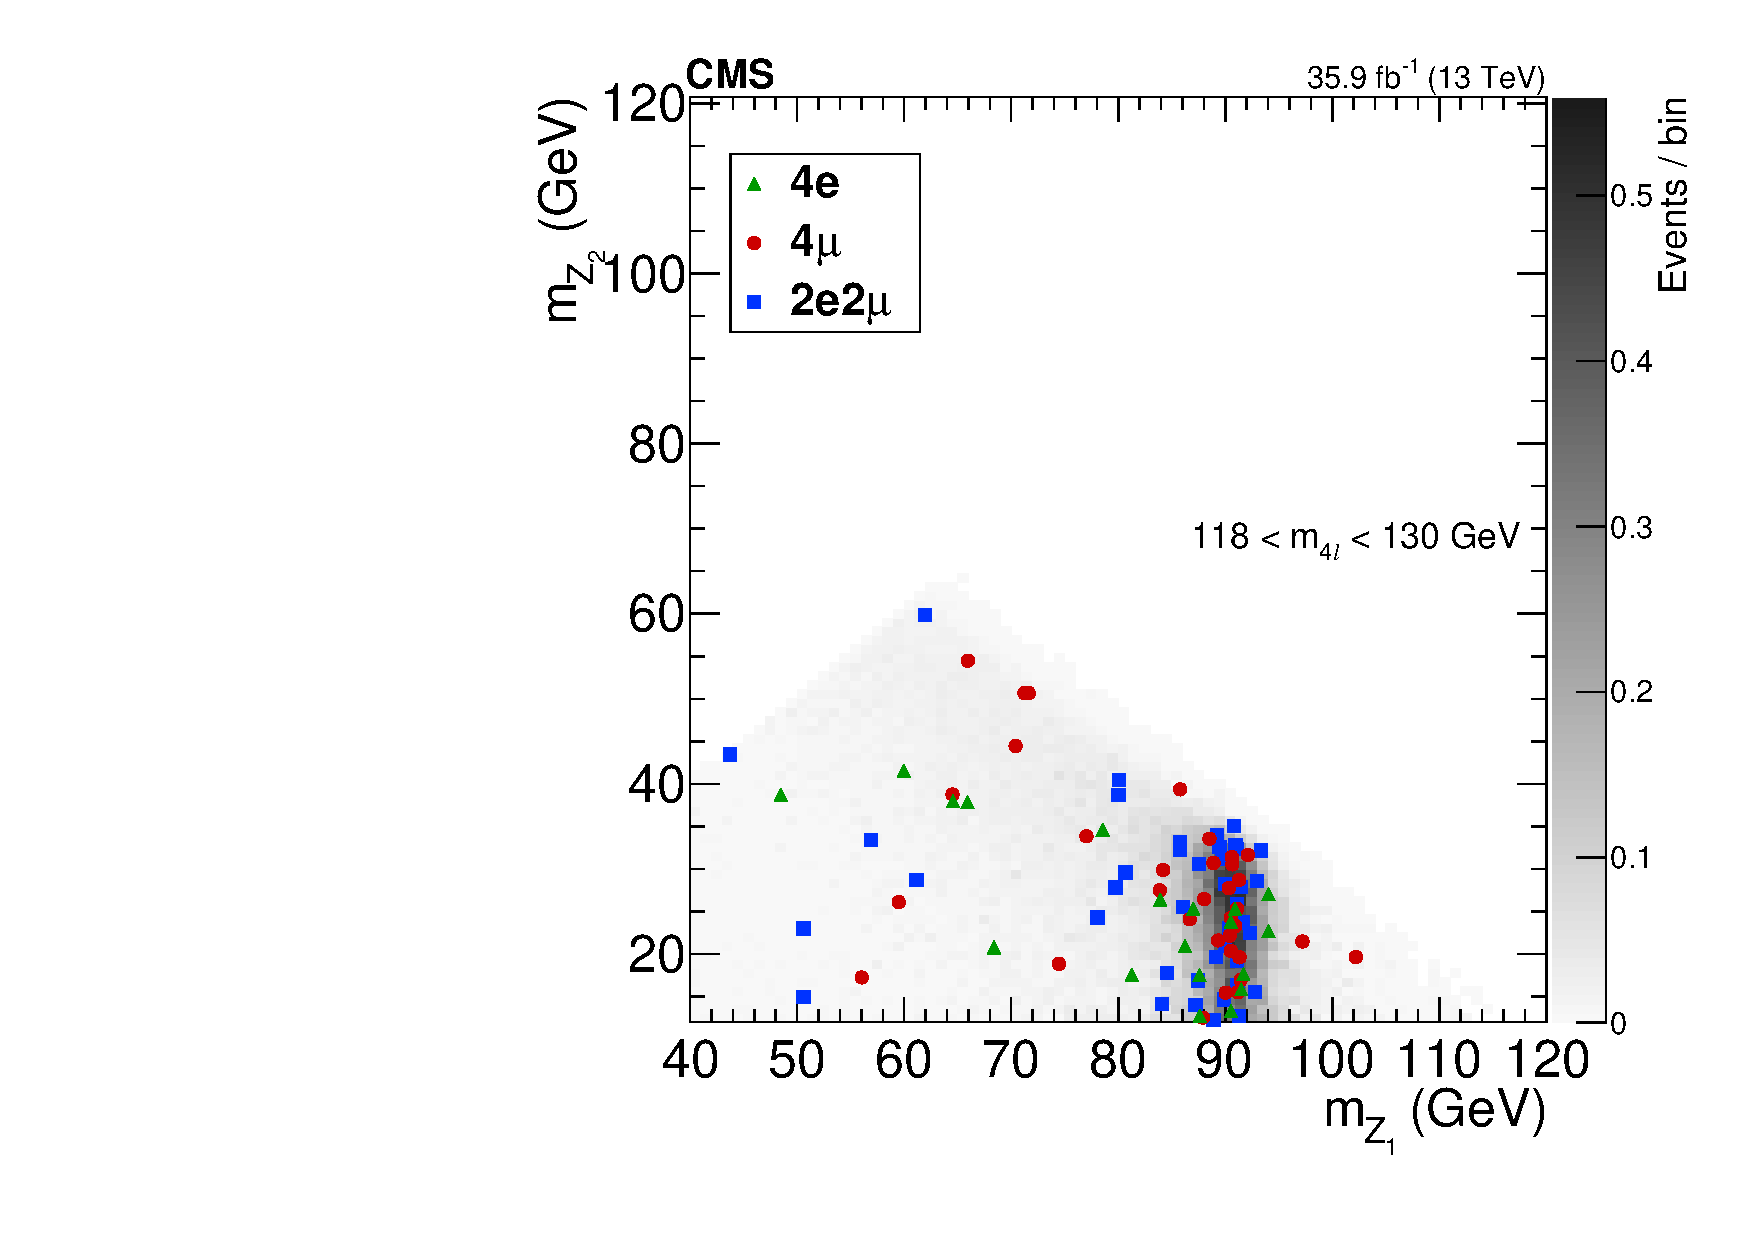
\includegraphics[width=0.75\textwidth]{results/mZ2VsmZ1_hzz.pdf}
    \caption[Scatter plot of $m_{\PZ_2}$ vs.\ $m_{\PZ_1}$ for data events near the Higgs resonance]{
        The reconstructed $m_{\PZ_2}$ mass plotted against the reconstructed $m_{\PZ_1}$ for data events in the Higgs selection with $118 < m_{4\ell} < 130\GeV$, with distinctive markers for each final state.
        The shading represents the expected number of events in the bin.
      }\label{fig:mZ2VsmZ1_hzz}
  \end{center}
\end{figure}


\subsection{ZZ Production}

Expected and observed yields for on-shell {\ZZ} events are shown in Table~\ref{tab:results_zz}.
The corresponding four-lepton and {\PZ} boson candidate invariant masses are shown in Figs.~\ref{fig:mass_smp} and~\ref{fig:zMass_smp}, respectively.
Figure~\ref{fig:njets} shows the distribution of the number of jets ($N_\text{jets}$) in these events.
The leading and subleading jet {\pt} are shown separately in Fig.~\ref{fig:jetPt}, and the leading and subleading jet {\abseta} are shown separately in Fig.~\ref{fig:jetEta}, for all events with at least one (leading) or two (subleading) jets.
Figures~\ref{fig:mjj} and~\ref{fig:deltaEtajj} show the $m_{\Pj\Pj}$ and $\lvert \Delta \eta_{\Pj\Pj} \rvert$ distributions for tagging jet pairs in the dijet selection.
Again, agreement is good overall, indicating that the observables shown are well modeled up to the precision achievable with current data.
These are the first such distributions published at $\sqrt{s} = 13\TeV$, and statistical uncertainties are smaller than those published at any energy, allowing theorists to make more detailed comparisons to their models and, in the case of the jet-related distributions, to QCD and shower modeling.

\begin{table}[htbp]
  \begin{center}
    \caption[Expected and observed yields for doubly-resonant {\ZZ} production.]{
      Observed and expected yields of {\ZZ} events, including expected background yields, in the on-shell selection, shown for each final state and summed to the total.
      Uncertainties are statistical, then systematic, not including the integrated luminosity uncertainty.
    }\label{tab:results_zz}
    \begin{tabular}{ccccc}
      \toprule
      Final & Expected   &  Background   & Total     & Observed \\
      state & $N_{\ZZ}$  &               & expected  &          \\
      \midrule
      \midrule
      $4\Pm$       & $ 301 \pm 2 \pm 9     $  & $ 10 \pm 1 \pm 2   $  & $ 311 \pm 2 \pm 9     $  & $ 335 $   \\
      $2\Pe 2\Pm$  & $ 503 \pm 2 \pm 19    $  & $ 31 \pm 2 \pm 4   $  & $ 534 \pm 3 \pm 20    $  & $ 543 $   \\
      $4\Pe$       & $ 205 \pm 1 \pm 12    $  & $ 20 \pm 2 \pm 2   $  & $ 225 \pm 2 \pm 13    $  & $ 220 $   \\
      \midrule
      Total        & $ 1009  \pm 3  \pm 36 $  & $ 60  \pm 3  \pm 8 $  & $ 1070  \pm 4  \pm 37 $  & $ 1098 $  \\
      \bottomrule
    \end{tabular}
  \end{center}
\end{table}

\begin{figure}[htbp]
  \begin{center}
    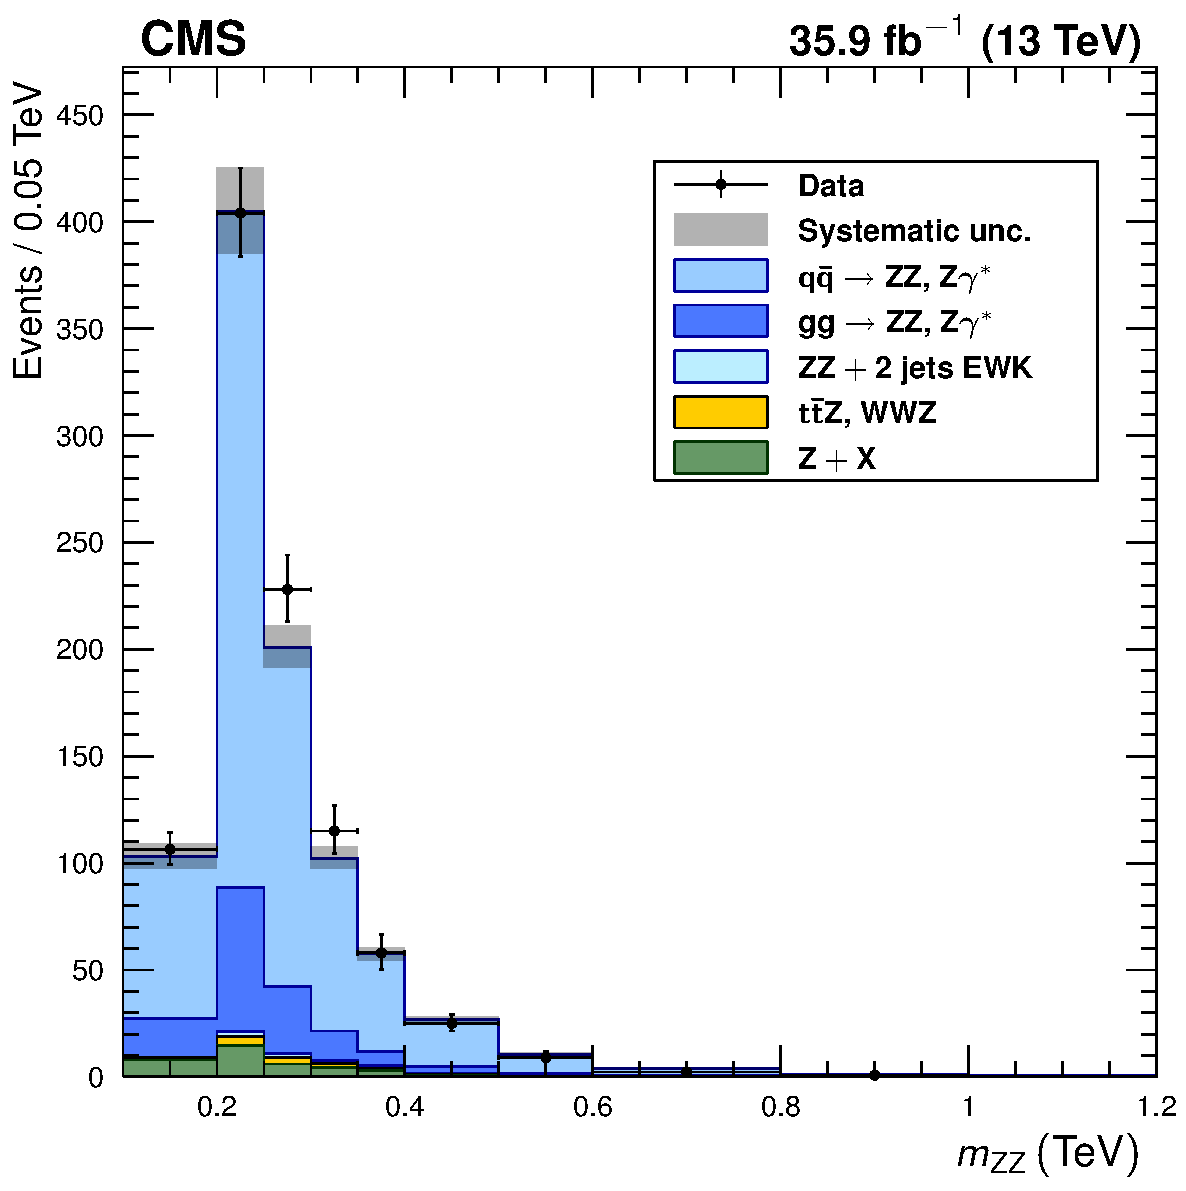
\includegraphics[width=0.75\textwidth]{results/smpzzMass.pdf}
    \caption[Four-lepton mass spectrum for events with both {\PZ} candidates on-shell]{
        Distribution of the four-lepton invariant mass $m_{\ZZ}$ of all events in the on-shell selection.
        Points represent data, with statistical uncertainty bars.
        The stack of filled histograms represents the SM signal prediction and background estimate, with a grey band showing the sum in quadrature of the statistical and systematic uncertainties on the total expected yield.
      }\label{fig:mass_smp}
  \end{center}
\end{figure}

\begin{figure}[htbp]
  \begin{center}
    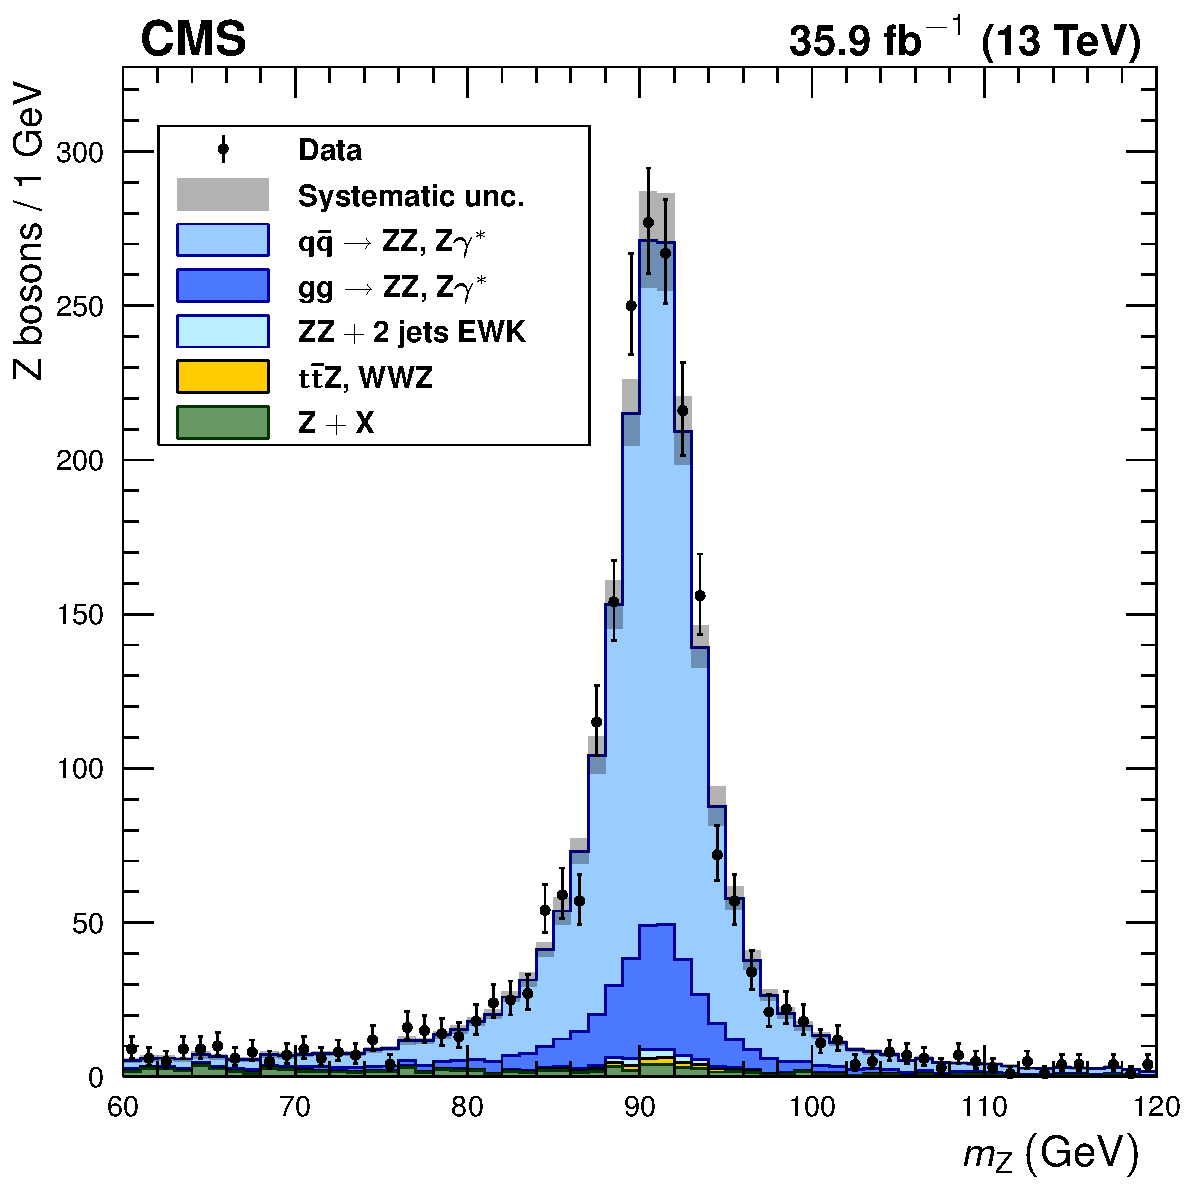
\includegraphics[width=0.75\textwidth]{results/smpzMass.pdf}
    \caption[Mass of all {\Zgs} candidates in the on-shell selection]{
        Distribution of the dilepton invariant mass of {\PZ} candidates in all events in the on-shell selection, regardless of whether the lepton pair is labeled $\PZ_1$ or $\PZ_2$.
        Points represent data, with statistical uncertainty bars.
        The stack of filled histograms represents the SM signal prediction and background estimate, with a grey band showing the sum in quadrature of the statistical and systematic uncertainties on the total expected yield.
      }\label{fig:zMass_smp}
  \end{center}
\end{figure}

\begin{figure}[htbp]
  \begin{center}
    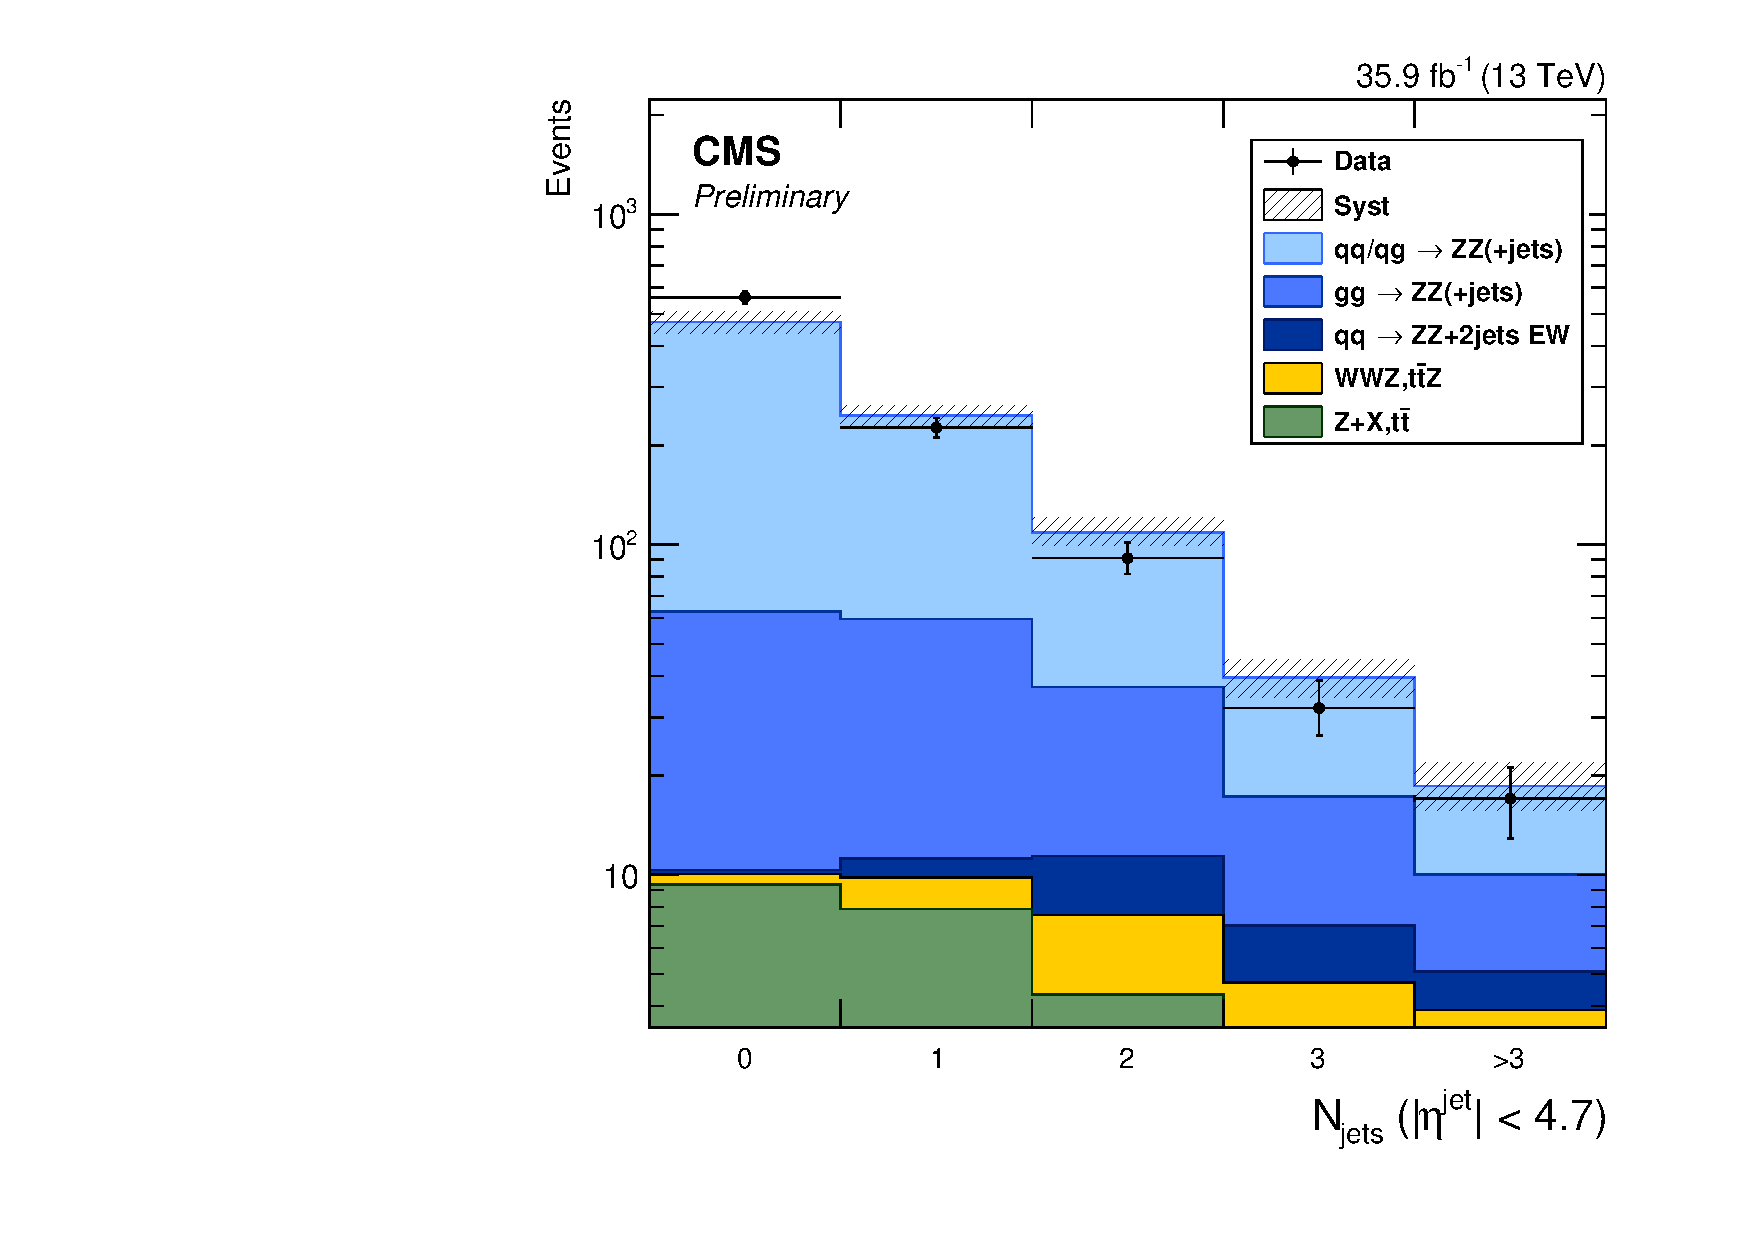
\includegraphics[width=0.75\textwidth]{results/njets.pdf}
    \caption[Jet multiplicity]{
        Distribution of jet multiplicity in {\ZZ} events.
        Points represent data, with statistical uncertainty bars.
        The stack of filled histograms represents the SM signal prediction and background estimate, with a hatched band showing the sum in quadrature of the statistical and systematic uncertainties on the total expected yield.
      }\label{fig:njets}
  \end{center}
\end{figure}

\begin{figure}[htbp]
  \begin{center}
    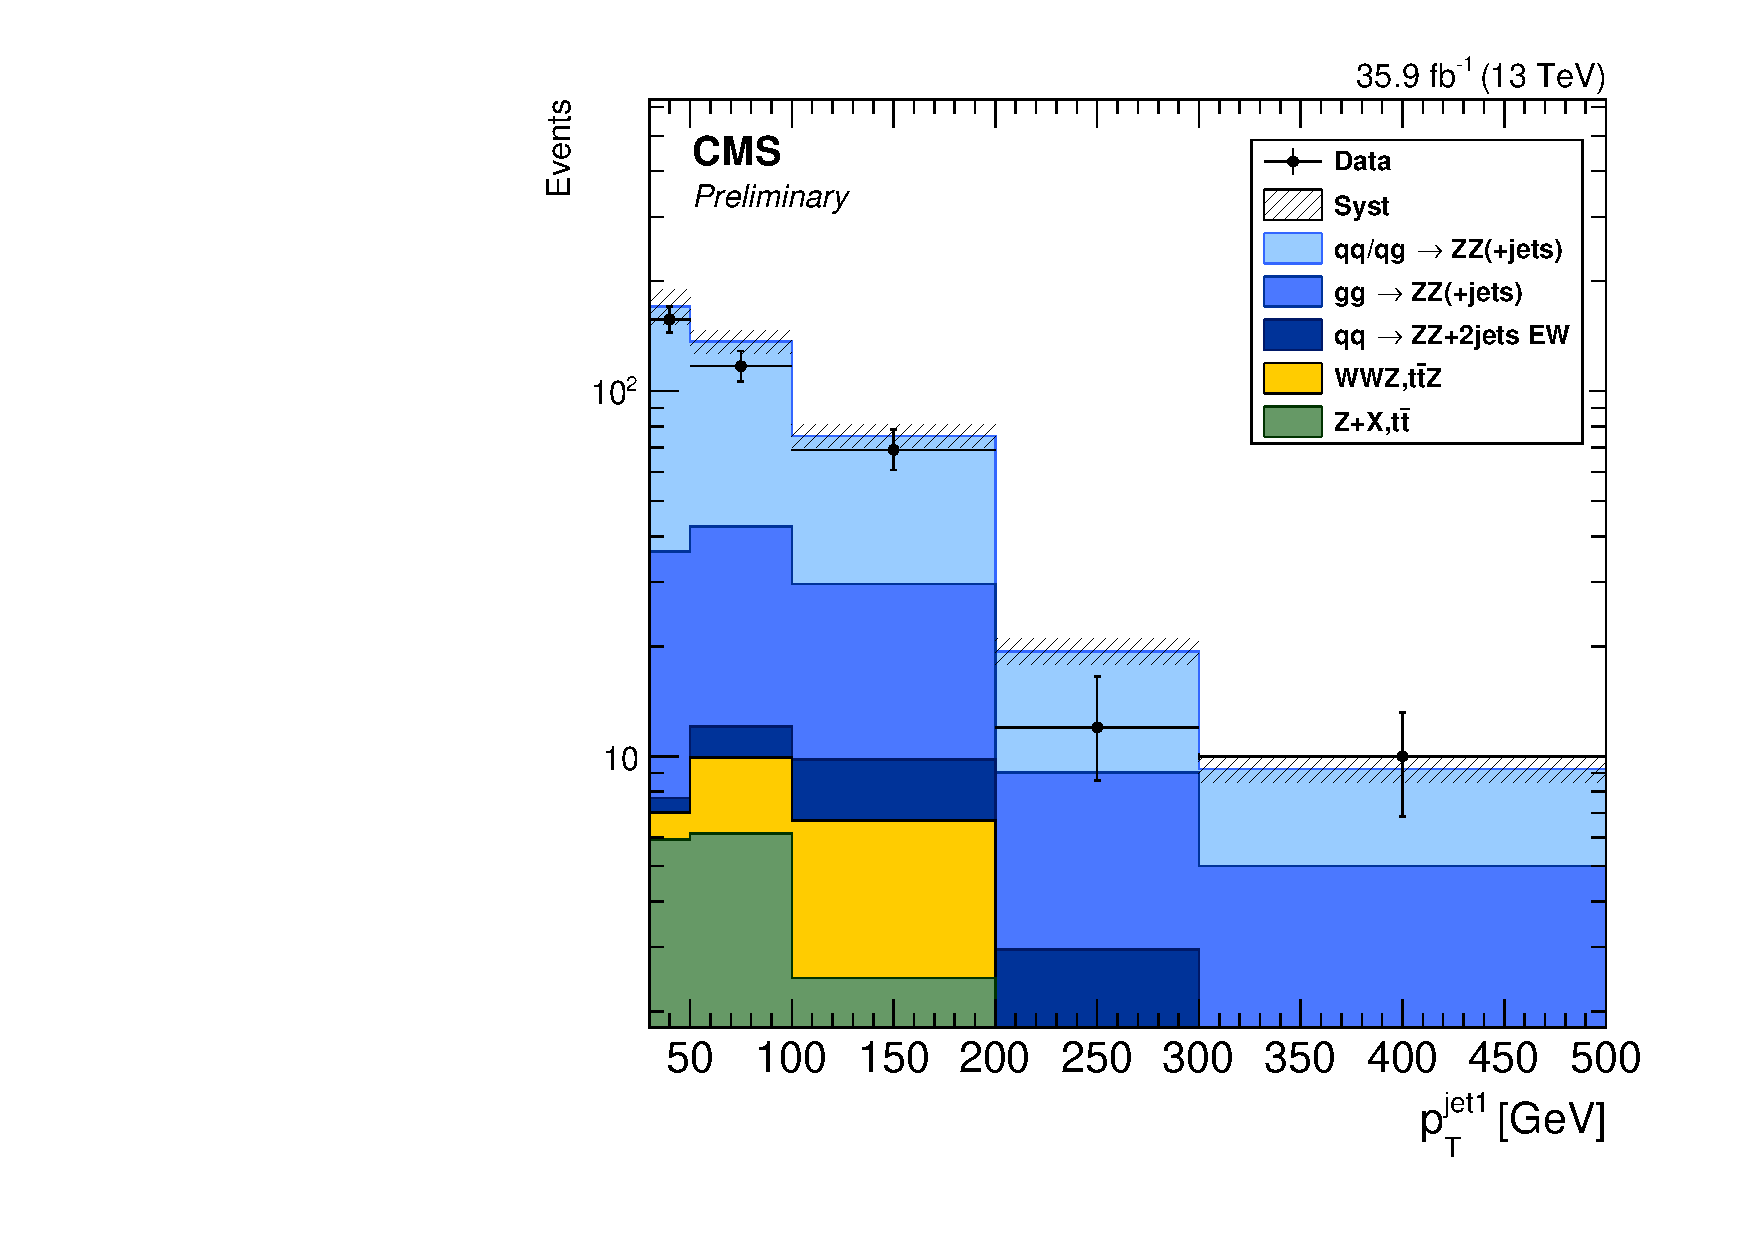
\includegraphics[width=0.48\textwidth]{results/j1Pt.pdf}
    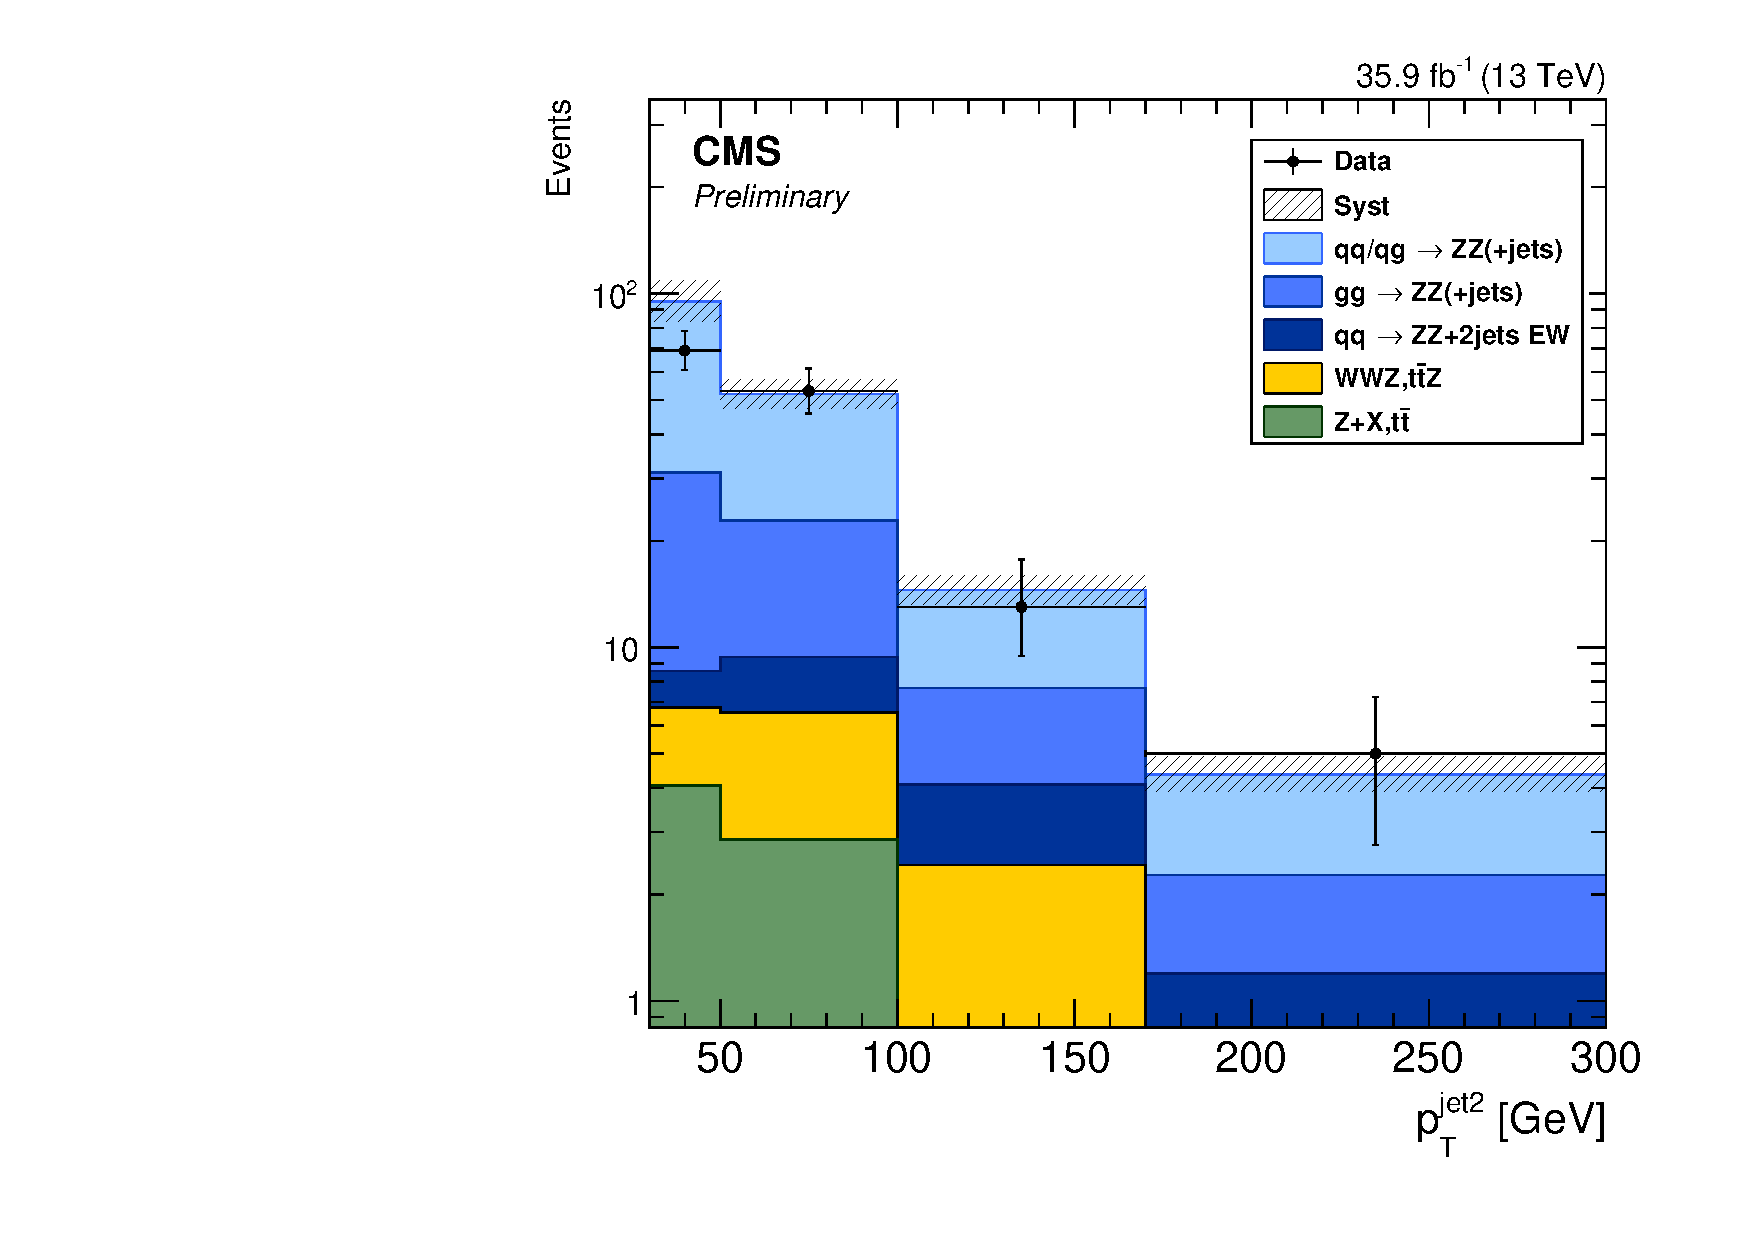
\includegraphics[width=0.48\textwidth]{results/j2Pt.pdf}
    \caption[Transverse momentum of the leading and subleading jets]{
        Distribution of leading (left) and subleading (right) jet {\pt} for all {\ZZ} events with at least one jet and at least two jets, respectively.
        Points represent data, with statistical uncertainty bars.
        The stack of filled histograms represents the SM signal prediction and background estimate, with a hatched band showing the sum in quadrature of the statistical and systematic uncertainties on the total expected yield.
      }\label{fig:jetPt}
  \end{center}
\end{figure}

\begin{figure}[htbp]
  \begin{center}
    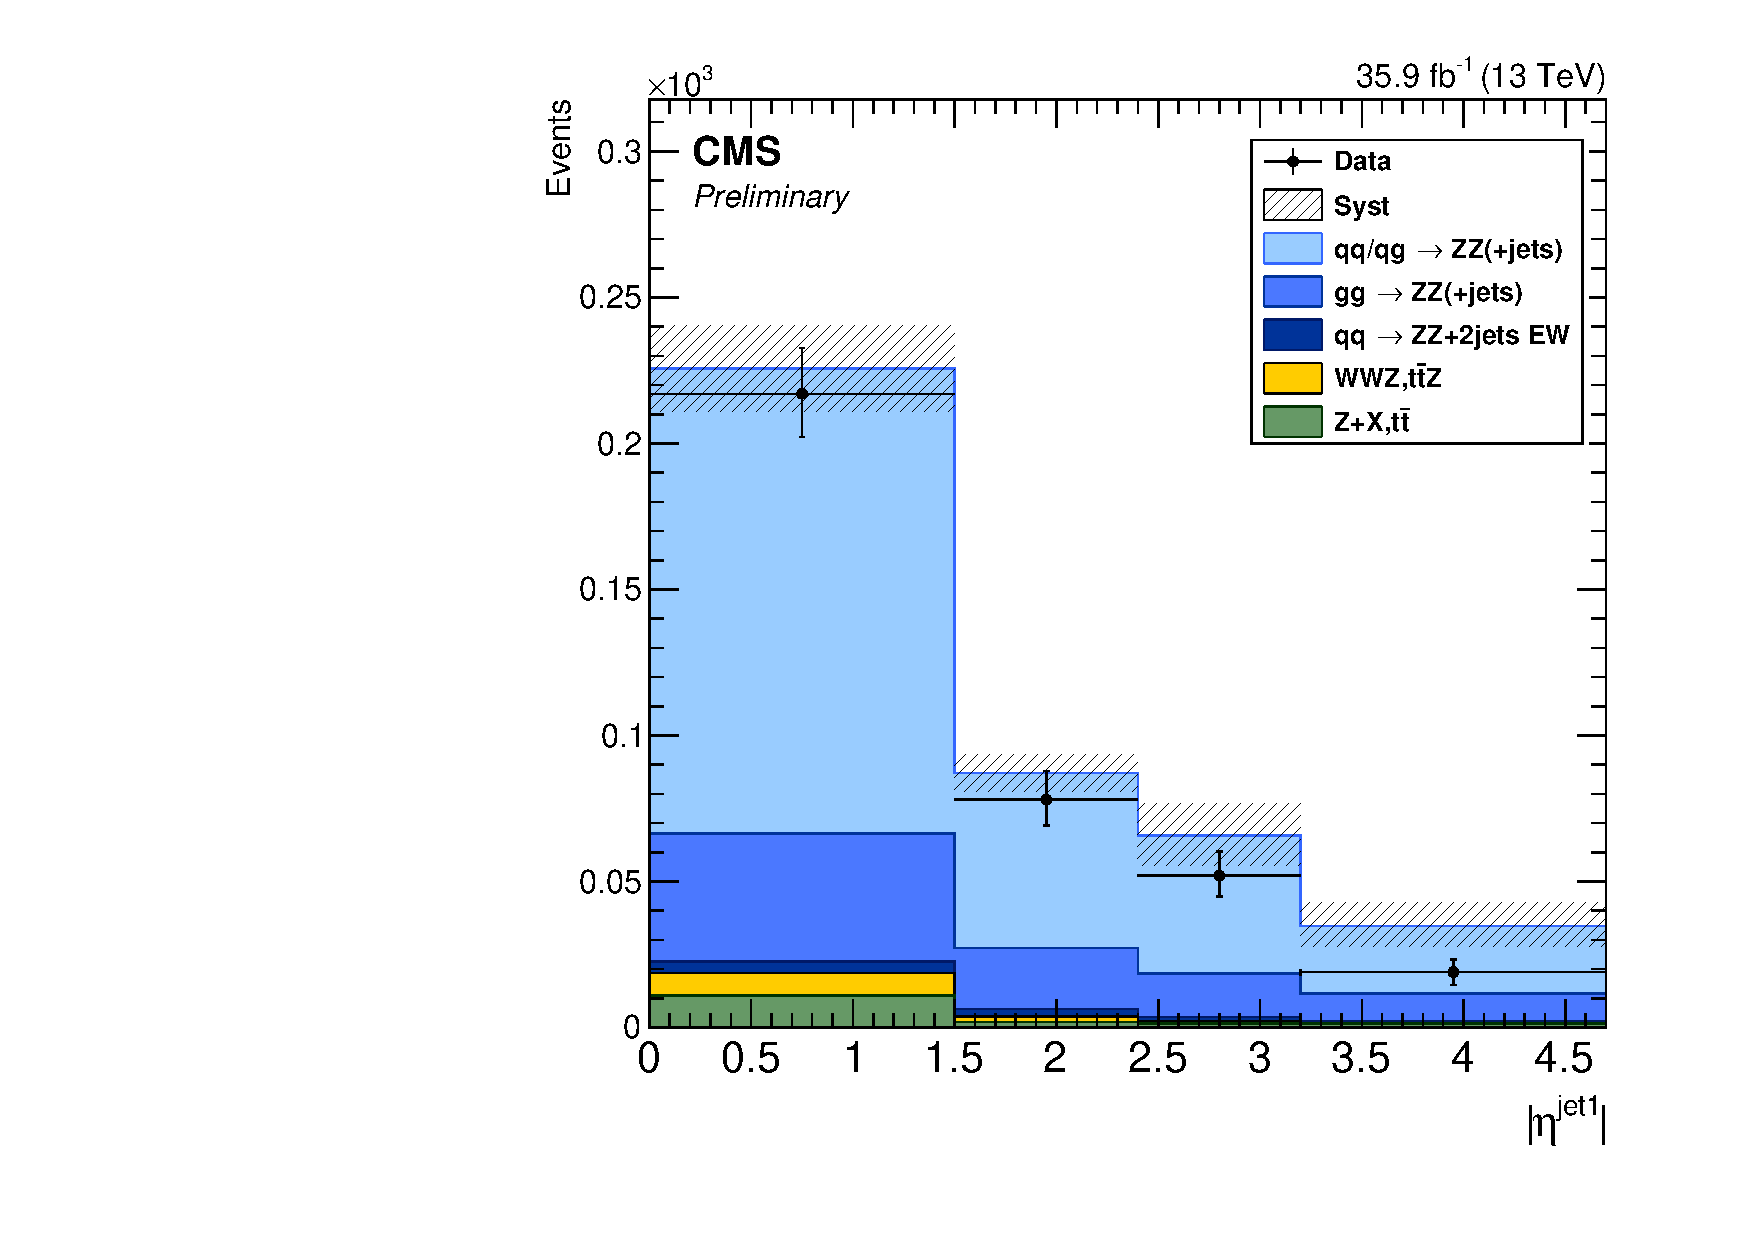
\includegraphics[width=0.48\textwidth]{results/j1Eta.pdf}
    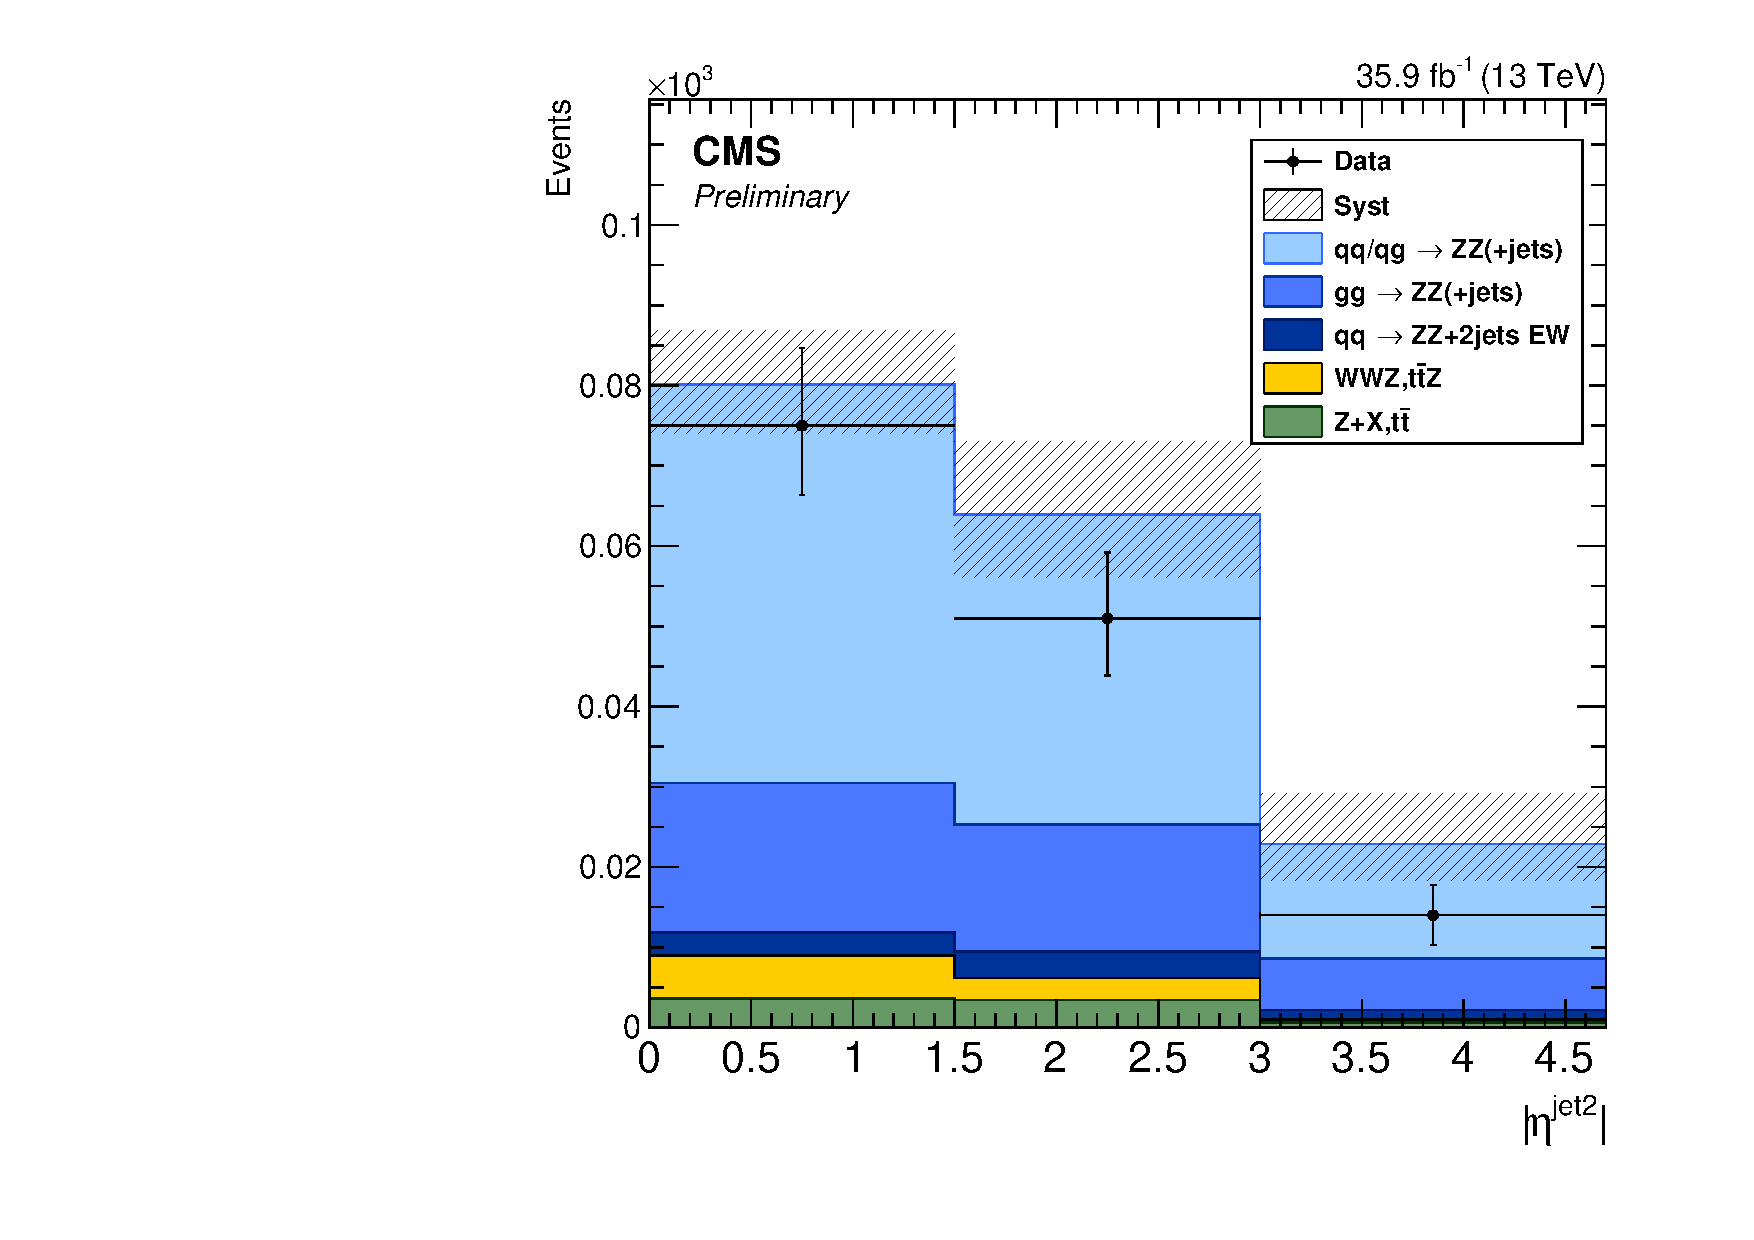
\includegraphics[width=0.48\textwidth]{results/j2Eta.pdf}
    \caption[Pseudorapidity of the leading and subleading jets]{
        Distribution of leading (left) and subleading (right) jet {\abseta} for all {\ZZ} events with at least one jet and at least two jets, respectively.
        Points represent data, with statistical uncertainty bars.
        The stack of filled histograms represents the SM signal prediction and background estimate, with a hatched band showing the sum in quadrature of the statistical and systematic uncertainties on the total expected yield.
      }\label{fig:jetEta}
  \end{center}
\end{figure}

\begin{figure}[htbp]
  \begin{center}
    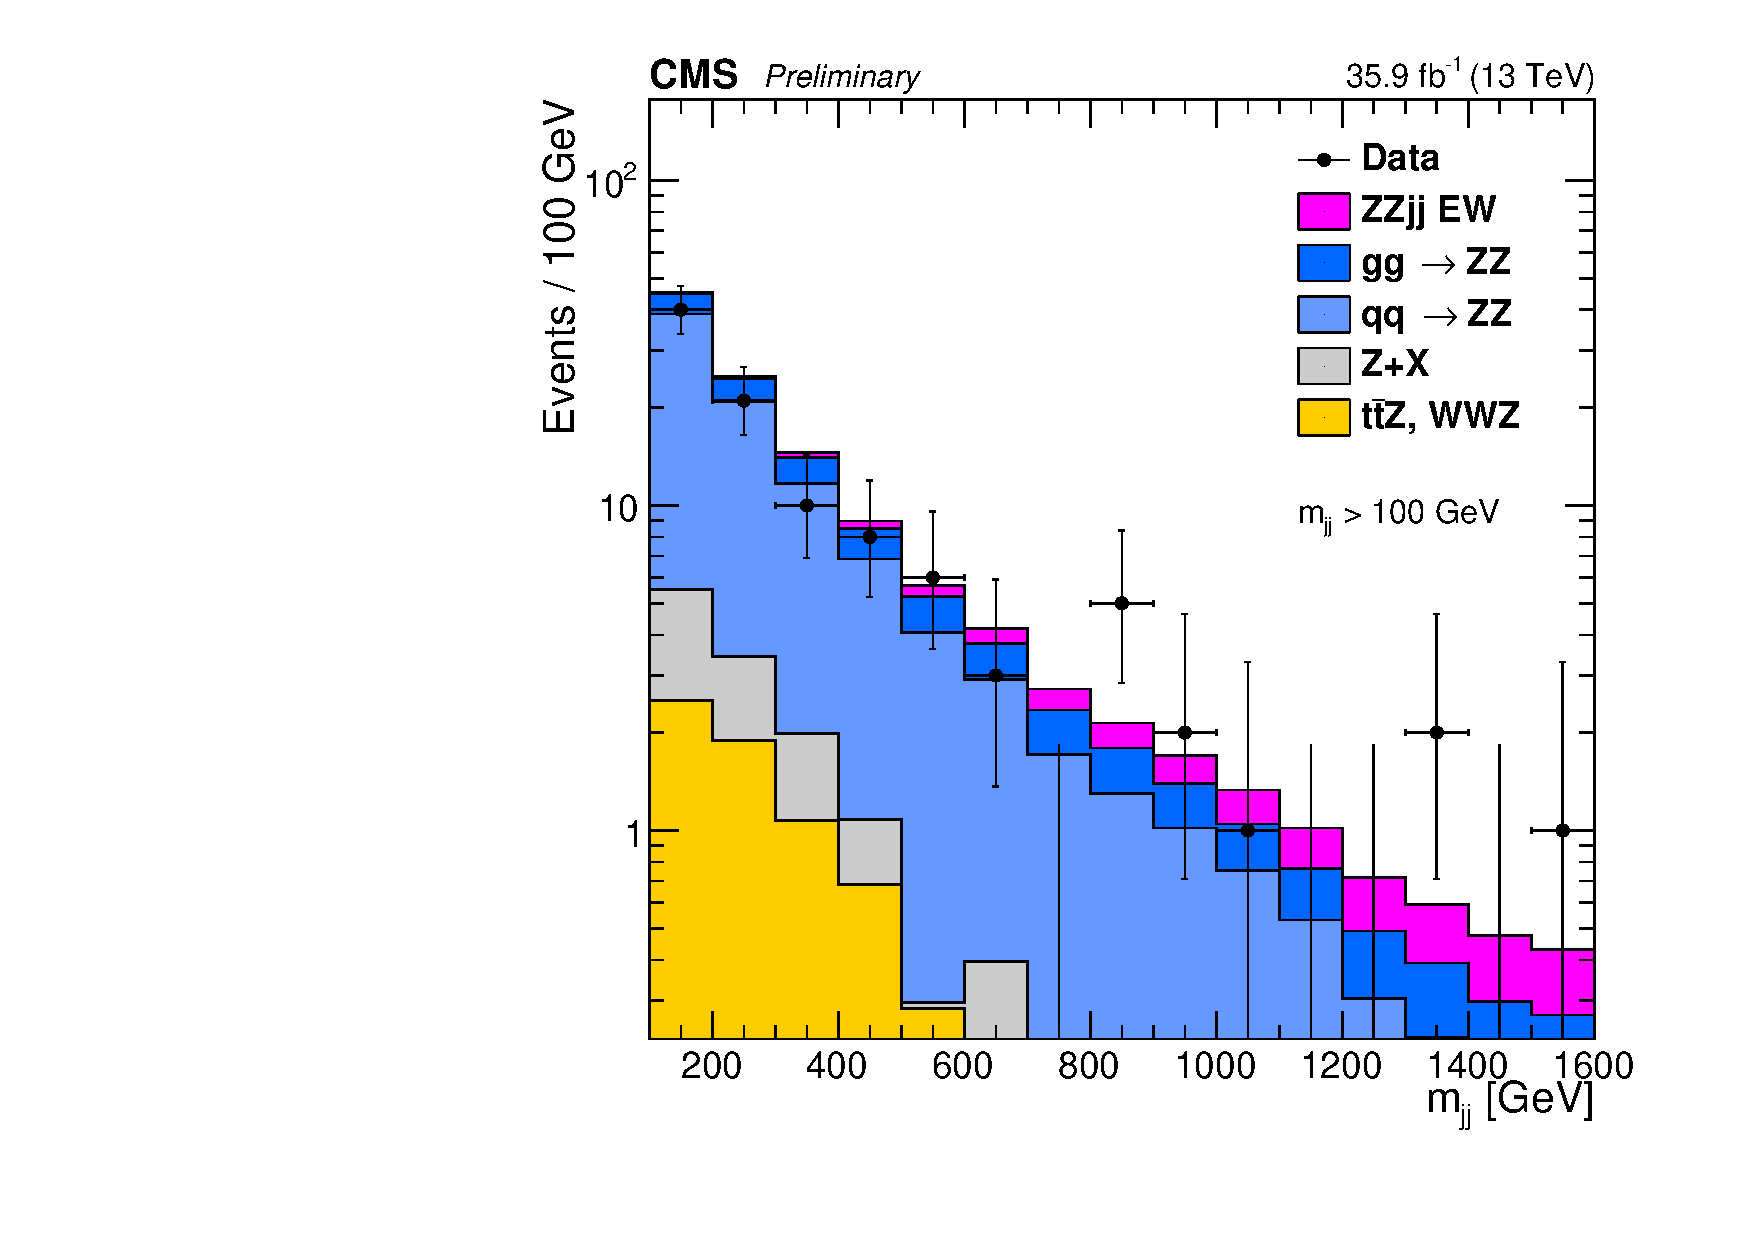
\includegraphics[width=0.75\textwidth]{results/mjj.pdf}
    \caption[Dijet invariant mass]{
        Dijet invariant mass $m_{\Pj\Pj}$ of the tag jets in {\ZZ} events passing the dijet selection ($m_{\Pj\Pj} > 100\GeV$).
        Points represent data, with statistical uncertainty bars.
        The stack of filled histograms represents the SM signal prediction, including EWK production, and background estimate.
      }\label{fig:mjj}
  \end{center}
\end{figure}

\begin{figure}[htbp]
  \begin{center}
    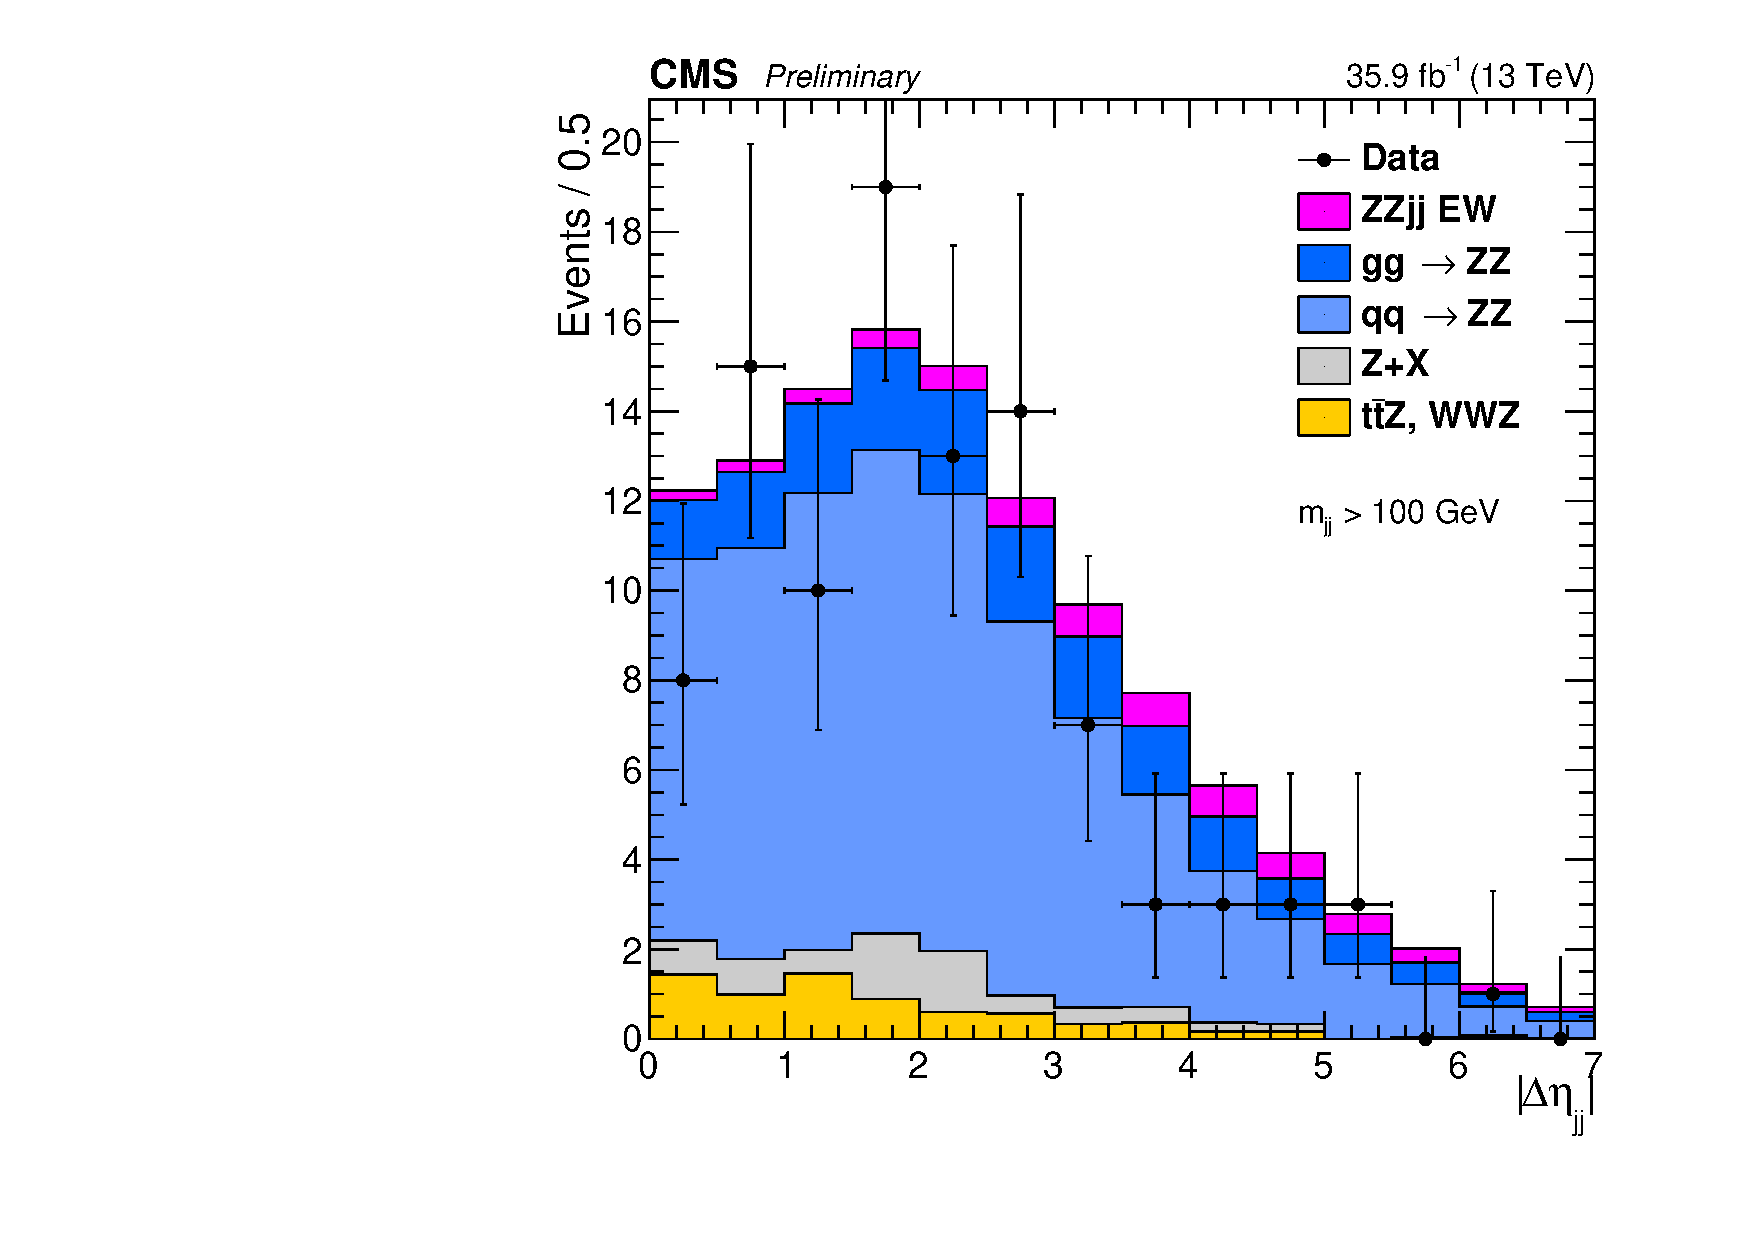
\includegraphics[width=0.75\textwidth]{results/deltaEtajj.pdf}
    \caption[Dijet pseudorapidity separation]{
        Pseudorapidity separation $\lvert \Delta \eta_{\Pj\Pj} \rvert$ of tag jets in {\ZZ} events passing the dijet selection ($m_{\Pj\Pj} > 100\GeV$).
        Points represent data, with statistical uncertainty bars.
        The stack of filled histograms represents the SM signal prediction, including EWK production, and background estimate.
      }\label{fig:deltaEtajj}
  \end{center}
\end{figure}


The yields shown in Table~\ref{tab:results_zz} and the systematic uncertainties of Table~\ref{tab:systematics} are used as inputs to the maximum likelihood method described in Section~\ref{sec:signalStrength} to obtain the on-shell {\ZZ} signal strength across all four-lepton final states,
\begin{equation}
  \mu = 1.040 _{-0.032}^{+0.033} \stat _{-0.035}^{+0.037} \syst \pm 0.026 \lum,
\end{equation}
which gives a fiducial cross section
\begin{equation}
  \sigma_\text{fid} (\pp \to \ZZ \to 4\ell) = 40.9 \pm 1.3 \stat \pm 1.4 \syst \pm 1.0 \lum \unit{fb},
\end{equation}
in the {\ZZfourl} fiducial phase space of Table~\ref{tab:fiducialDefs}.
The corresponding total cross section is
\begin{equation}
  \sigma(\pp \to \ZZ) = 17.5 _{-0.5}^{+0.6} \stat \pm 0.6 \syst \pm 0.4 \thy \pm 0.4 \lum \unit{pb}.
\end{equation}

This measurement, on 2016 data, agrees with the result of the 2015 measurement~\cite{Khachatryan:2016txa},
\begin{equation}
  \sigma(\pp \to \ZZ) = 14.6 ^{+1.9}_{-1.8} \stat _{-0.5}^{+0.3} \syst \pm 0.2 \thy \pm 0.4 \lum \unit{pb}.
\end{equation}
One may combine the measurements by doing a six-bin simultaneous fit with the bins representing the same final state in 2015 and 2016 considered separately.
The degree of correlation between the systematic uncertainties in the 2015 and 2016 runs is not known, but the 2015 contribution is small enough that the systematic uncertainties are dominated by those in the 2016 dataset, and the degree of correlation will have only a small effect on the measurement.
We therefore do the fit twice, once treating the experimental uncertainties as fully correlated between the datasets, and again treating them as fully uncorrelated.
The small difference in the central value obtained is added linearly to the systematic error of the result.
After the full combination, the ``$2015 + 2016$'' total cross section is found to be
\begin{equation}
  \sigma(\pp \to \ZZ) = 17.2 \pm 0.5 \stat \pm 0.7 \syst \pm 0.4 \thy \pm 0.4 \lum \unit{pb}.
\end{equation}
These results can be compared to the {\MATRIX}~v1.0.0\_beta4 prediction of $16.2^{+0.6}_{-0.4}\unit{pb}$, computed at NNLO in QCD, or the {\MCFM}~v7.0 prediction of $15.0^{+0.7}_{-0.6} \pm 0.2\unit{pb}$, calculated at NLO in QCD with LO $\Pg\Pg \to \ZZ$ diagrams included.
Both predictions use the NNPDF3.0 PDF sets and fixed scales $\mu_\text{F} = \mu_\text{R} = m_\PZ$.

The total cross section is shown as a function of $\sqrt{s}$ in Fig.~\ref{fig:xsec_vs_sqrts}.
Measurements from CMS~\cite{Chatrchyan:2012sga,CMS:2014xja,Khachatryan:2015pba,Khachatryan:2016txa} and ATLAS~\cite{Aad:2012awa,Aad:2015rka,Aad:2015zqe} are compared to NLO predictions made with {\MCFM} (with contributions from leading order gluon-gluon fusion diagrams), and NNLO predictions made with {\MATRIX}.
Results from both experiments agree with the predictions, verifying this aspect of the SM to within the measurements' uncertainties.

\begin{figure}[htbp]
  \begin{center}
    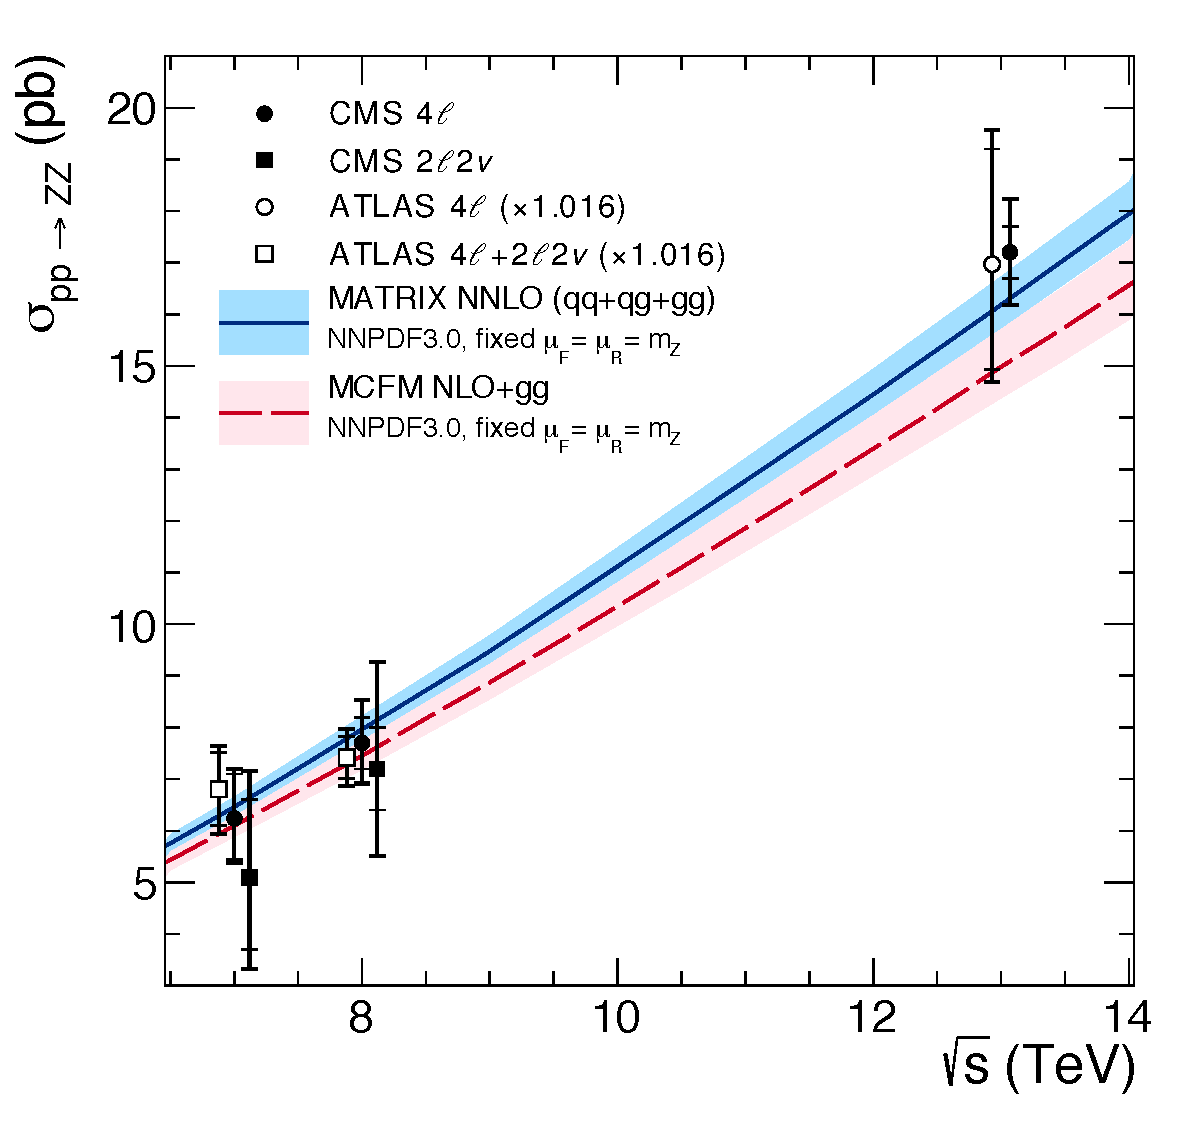
\includegraphics[width=0.95\textwidth]{results/sqrts.pdf}
    \caption[Total {\ZZ} cross section as a function of center-of-mass energy]{
        The total {\ZZ} cross section is shown as a function of $\sqrt{s}$.
        Measurements from CMS and ATLAS are both shown, with the ATLAS numbers adjusted upward by 1.6\% to account for differences in {\PZ} mass window choice.
        Points at the same center-of-mass energy are shifted slightly in the horizontal direction for clarity.
        Experimental measurements are compared to predictions from {\MCFM} at NLO in QCD with additional contributions from LO gluon-gluon fusion diagrams, and {\MATRIX} at NNLO in QCD\@.
        Both sets of predictions use the NNPDF3.0 PDF sets and fixed scales $\mu_\text{F} = \mu_\text{R} = m_\PZ$.
      }\label{fig:xsec_vs_sqrts}
  \end{center}
\end{figure}



\section{Differential Cross Sections}

Detector-level distributions are unfolded to calculate differential cross sections as described in Section~\ref{sec:diffXSec}.
Figures~\ref{fig:unfold_mass}--\ref{fig:unfold_massFull} show measured differential cross sections and corresponding theory predictions, as functions of different observables.
All distributions are normalized to the inclusive fiducial cross section, such that the integral of each is unity, including overflow bins (not shown).
The observables in Figs.~\ref{fig:unfold_mass}--\ref{fig:unfold_deltaPhiZZ} consider only the four-lepton system.
For the calculation of these distributions, as well as the differential cross section as a function of $N_\text{jets}$ (Fig.~\ref{fig:unfold_njets}), all events passing the on-shell selection of Table~\ref{tab:fiducialDefs} are used.
Figures~\ref{fig:unfold_mjj} and~\ref{fig:unfold_deltaEtajj} show $m_{\Pj\Pj}$ and $\lvert \Delta \eta_{\Pj\Pj} \rvert$ for all {\ZZ} events with at least two jets, while Figs~\ref{fig:unfold_jPt} and~\ref{fig:unfold_jEta} show {\pt} and $\eta$, respectively, for the leading jet in events with $N_\text{jets} \geq 1$ on the left and the subleading jet in events with $N_\text{jets} \geq 2$ on the right.
In Fig.~\ref{fig:unfold_massFull}, the phase space is expanded to the full spectrum selection of Table~\ref{tab:fiducialDefs} at both detector and true level, to show the four-lepton differential cross section through all production modes as a function of $m_{4\ell}$.
Measured cross sections overall agree with the theoretical predictions within their uncertainties, which are dominated by statistical uncertainties in all bins.


\begin{figure}[htbp]
  \begin{center}
    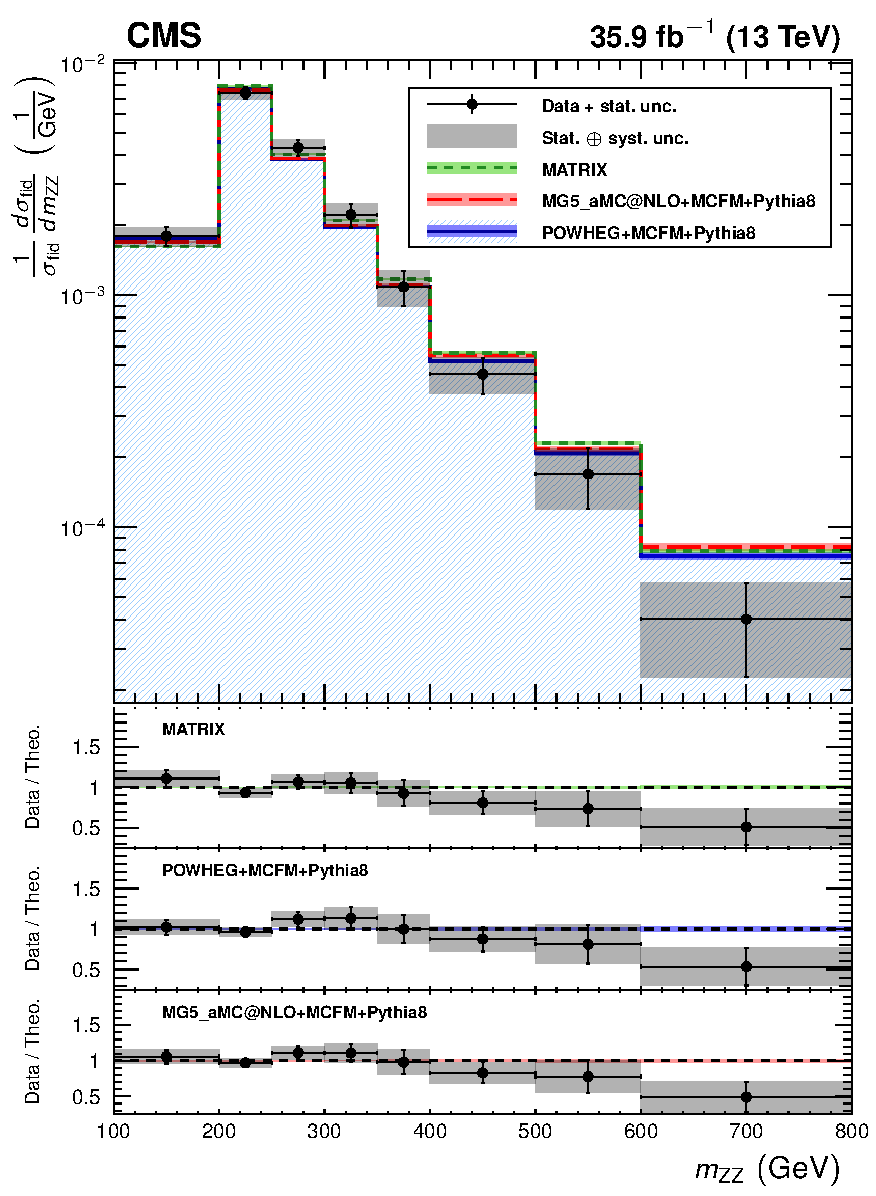
\includegraphics[width=0.78\textwidth]{results/unfold_mass.pdf}
    \caption[Normalized differential {\ZZ} cross section as a function of four-lepton invariant mass]{
        The {\ZZ} differential cross section as a function of $m_{\ZZ}$, normalized to the inclusive fiducial cross section.
        Points represent the unfolded data, with vertical bars showing the statistical uncertainty and a grey band showing the sum in quadrature of the statistical and systematic uncertainties.
        Blue, red, and green histograms represent the {\POWHEG}+{\MCFM}, {\MGAMC}+{\MCFM}, and {\MATRIX} predictions, respectively, with bands around each which represent their combined statistical, scale, and PDF uncertainties.
        The lower sections of the plot represents the ratio of the measured cross section to each of the predictions.
      }\label{fig:unfold_mass}
  \end{center}
\end{figure}

\begin{figure}[htbp]
  \begin{center}
    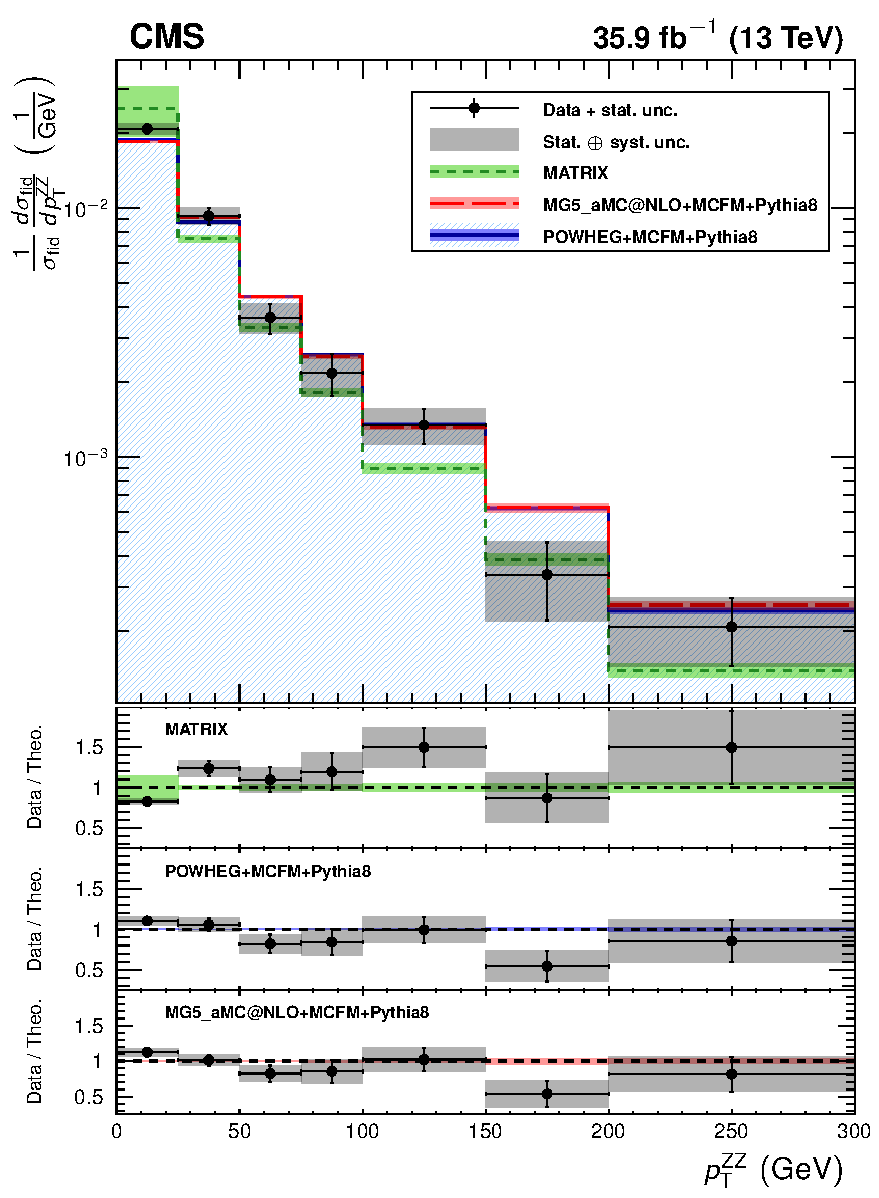
\includegraphics[width=0.78\textwidth]{results/unfold_pt.pdf}
    \caption[Normalized differential {\ZZ} cross section as a function of four-lepton system {\pt}]{
        The {\ZZ} differential cross section as a function of the four-lepton {\pt}, normalized to the inclusive fiducial cross section.
        Points represent the unfolded data, with vertical bars showing the statistical uncertainty and a grey band showing the sum in quadrature of the statistical and systematic uncertainties.
        Blue, red, and green histograms represent the {\POWHEG}+{\MCFM}, {\MGAMC}+{\MCFM}, and {\MATRIX} predictions, respectively, with bands around each which represent their combined statistical, scale, and PDF uncertainties.
        The lower sections of the plot represents the ratio of the measured cross section to each of the predictions.
      }\label{fig:unfold_pt}
  \end{center}
\end{figure}

\begin{figure}[htbp]
  \begin{center}
    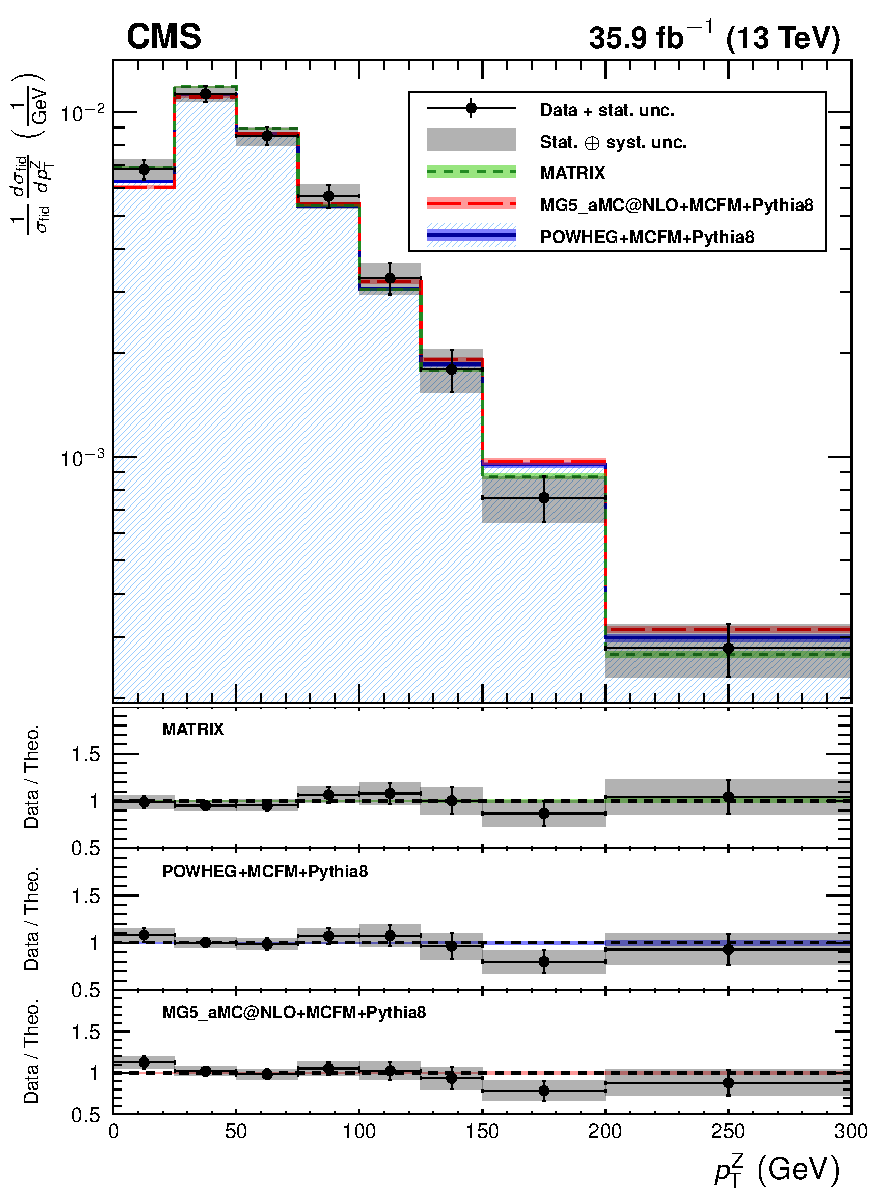
\includegraphics[width=0.78\textwidth]{results/unfold_zPt.pdf}
    \caption[Normalized differential {\ZZ} cross section as a function of {\PZ} boson candidate {\pt}]{
        The {\ZZ} differential cross section as a function of the {\pt} of both {\PZ} boson candidates, regardless of which one is $\PZ_1$ and which is $\PZ_2$, normalized to the inclusive fiducial cross section.
        Points represent the unfolded data, with vertical bars showing the statistical uncertainty and a grey band showing the sum in quadrature of the statistical and systematic uncertainties.
        Blue, red, and green histograms represent the {\POWHEG}+{\MCFM}, {\MGAMC}+{\MCFM}, and {\MATRIX} predictions, respectively, with bands around each which represent their combined statistical, scale, and PDF uncertainties.
        The lower sections of the plot represents the ratio of the measured cross section to each of the predictions.
      }\label{fig:unfold_zPt}
  \end{center}
\end{figure}

\begin{figure}[htbp]
  \begin{center}
    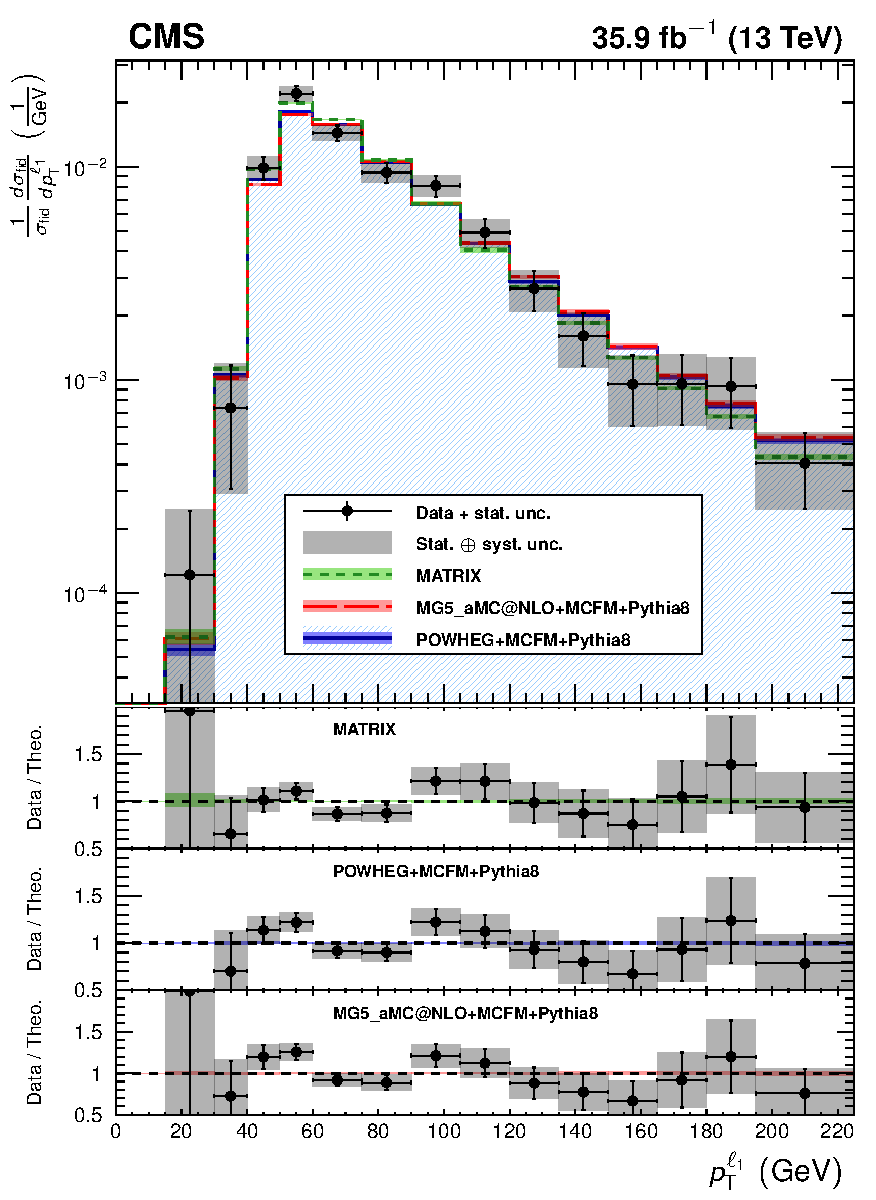
\includegraphics[width=0.78\textwidth]{results/unfold_l1Pt.pdf}
    \caption[Normalized differential {\ZZ} cross section as a function of leading lepton {\pt}]{
        The {\ZZ} differential cross section as a function of leading lepton {\pt}, normalized to the inclusive fiducial cross section.
        Points represent the unfolded data, with vertical bars showing the statistical uncertainty and a grey band showing the sum in quadrature of the statistical and systematic uncertainties.
        Blue, red, and green histograms represent the {\POWHEG}+{\MCFM}, {\MGAMC}+{\MCFM}, and {\MATRIX} predictions, respectively, with bands around each which represent their combined statistical, scale, and PDF uncertainties.
        The lower sections of the plot represents the ratio of the measured cross section to each of the predictions.
      }\label{fig:unfold_l1Pt}
  \end{center}
\end{figure}

\begin{figure}[htbp]
  \begin{center}
    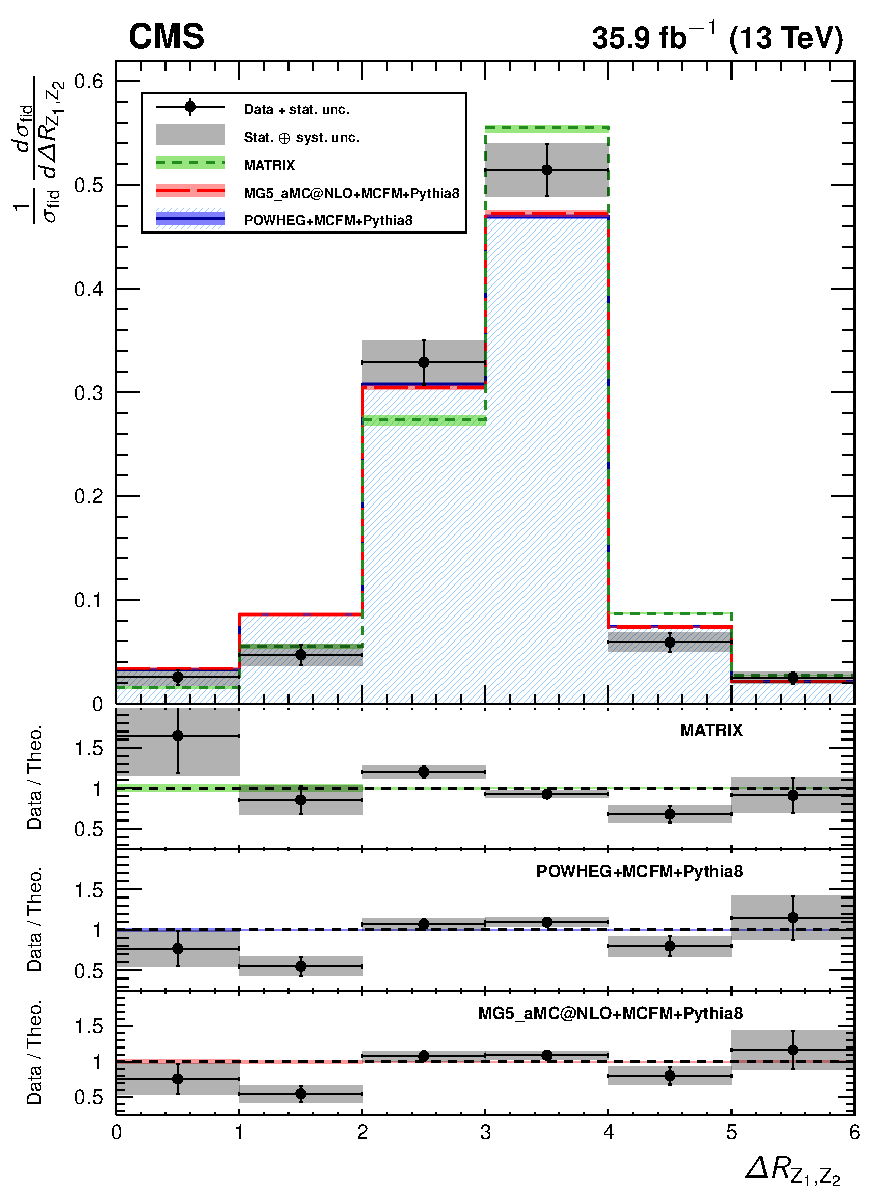
\includegraphics[width=0.78\textwidth]{results/unfold_deltaRZZ.pdf}
    \caption[Normalized differential {\ZZ} cross section as a function of $\Delta R$ between the {\PZ} bosons]{
        The {\ZZ} differential cross section as a function of $\Delta R$ between the two {\PZ} bosons, normalized to the inclusive fiducial cross section.
        Points represent the unfolded data, with vertical bars showing the statistical uncertainty and a grey band showing the sum in quadrature of the statistical and systematic uncertainties.
        Blue, red, and green histograms represent the {\POWHEG}+{\MCFM}, {\MGAMC}+{\MCFM}, and {\MATRIX} predictions, respectively, with bands around each which represent their combined statistical, scale, and PDF uncertainties.
        The lower sections of the plot represents the ratio of the measured cross section to each of the predictions.
      }\label{fig:unfold_deltaRZZ}
  \end{center}
\end{figure}

\begin{figure}[htbp]
  \begin{center}
    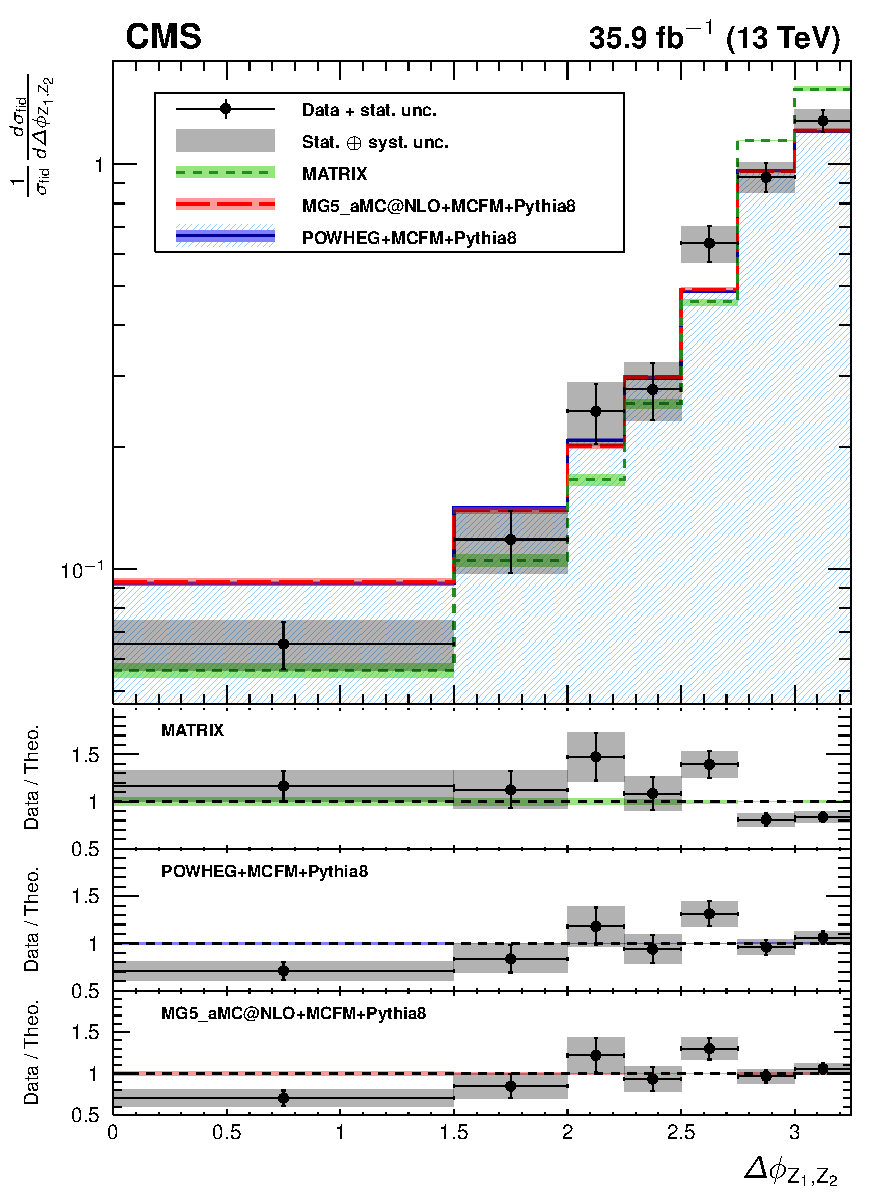
\includegraphics[width=0.78\textwidth]{results/unfold_deltaPhiZZ.pdf}
    \caption[Normalized differential {\ZZ} cross section as a function of $\Delta \phi$ between the {\PZ} bosons]{
        The {\ZZ} differential cross section as a function of $\Delta \phi$ between the two {\PZ} bosons, normalized to the inclusive fiducial cross section.
        Points represent the unfolded data, with vertical bars showing the statistical uncertainty and a grey band showing the sum in quadrature of the statistical and systematic uncertainties.
        Blue, red, and green histograms represent the {\POWHEG}+{\MCFM}, {\MGAMC}+{\MCFM}, and {\MATRIX} predictions, respectively, with bands around each which represent their combined statistical, scale, and PDF uncertainties.
        The lower sections of the plot represents the ratio of the measured cross section to each of the predictions.
      }\label{fig:unfold_deltaPhiZZ}
  \end{center}
\end{figure}

\begin{figure}[htbp]
  \begin{center}
    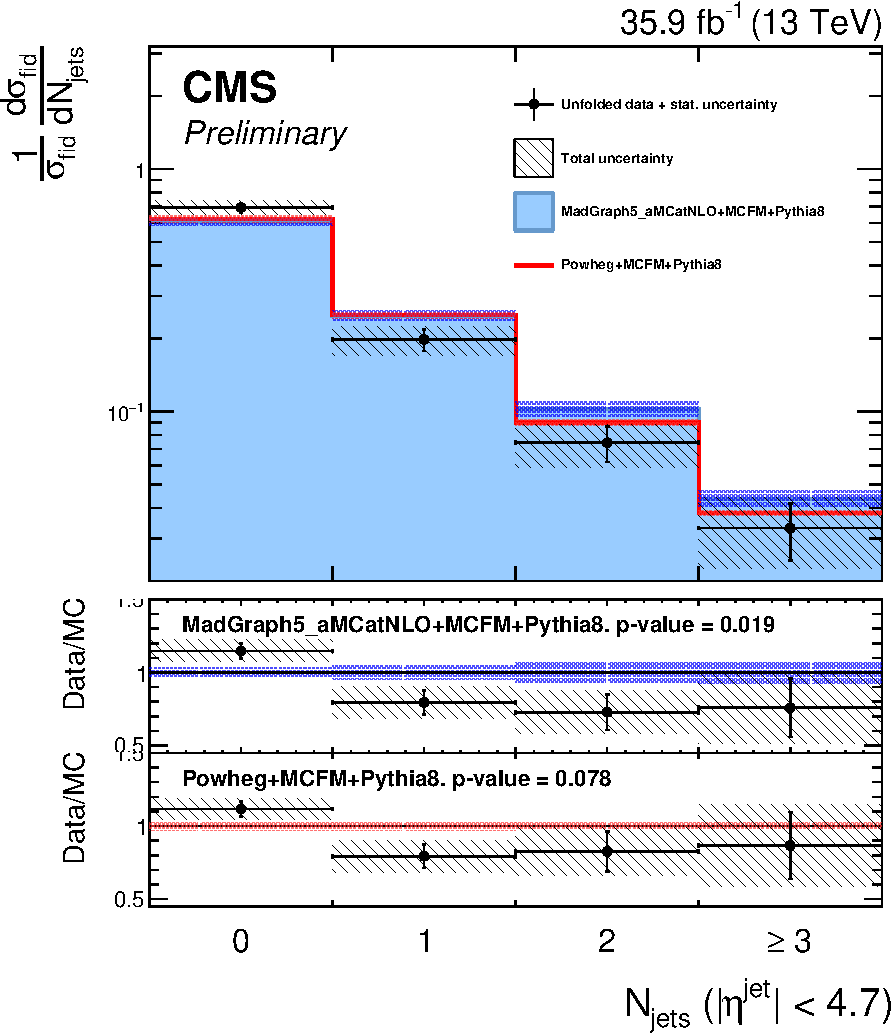
\includegraphics[width=0.88\textwidth]{results/unfold_njets.pdf}
    \caption[Normalized differential {\ZZ} cross section as a function of jet multiplicity]{
        The {\ZZ} differential cross section as a function of the jet multiplicity $N_\text{jets}$, normalized to the inclusive fiducial cross section.
        Points represent the unfolded data, with vertical bars showing the statistical uncertainty and a hatched band showing the sum in quadrature of the statistical and systematic uncertainties.
        Red and blue histograms represent the {\POWHEG}+{\MCFM} and {\MGAMC}+{\MCFM} predictions, respectively, with bands around each which represent their combined statistical, scale, and PDF uncertainties.
        The lower sections of the plot represents the ratio of the measured cross section to each of the predictions.
      }\label{fig:unfold_njets}
  \end{center}
\end{figure}

\begin{figure}[htbp]
  \begin{center}
    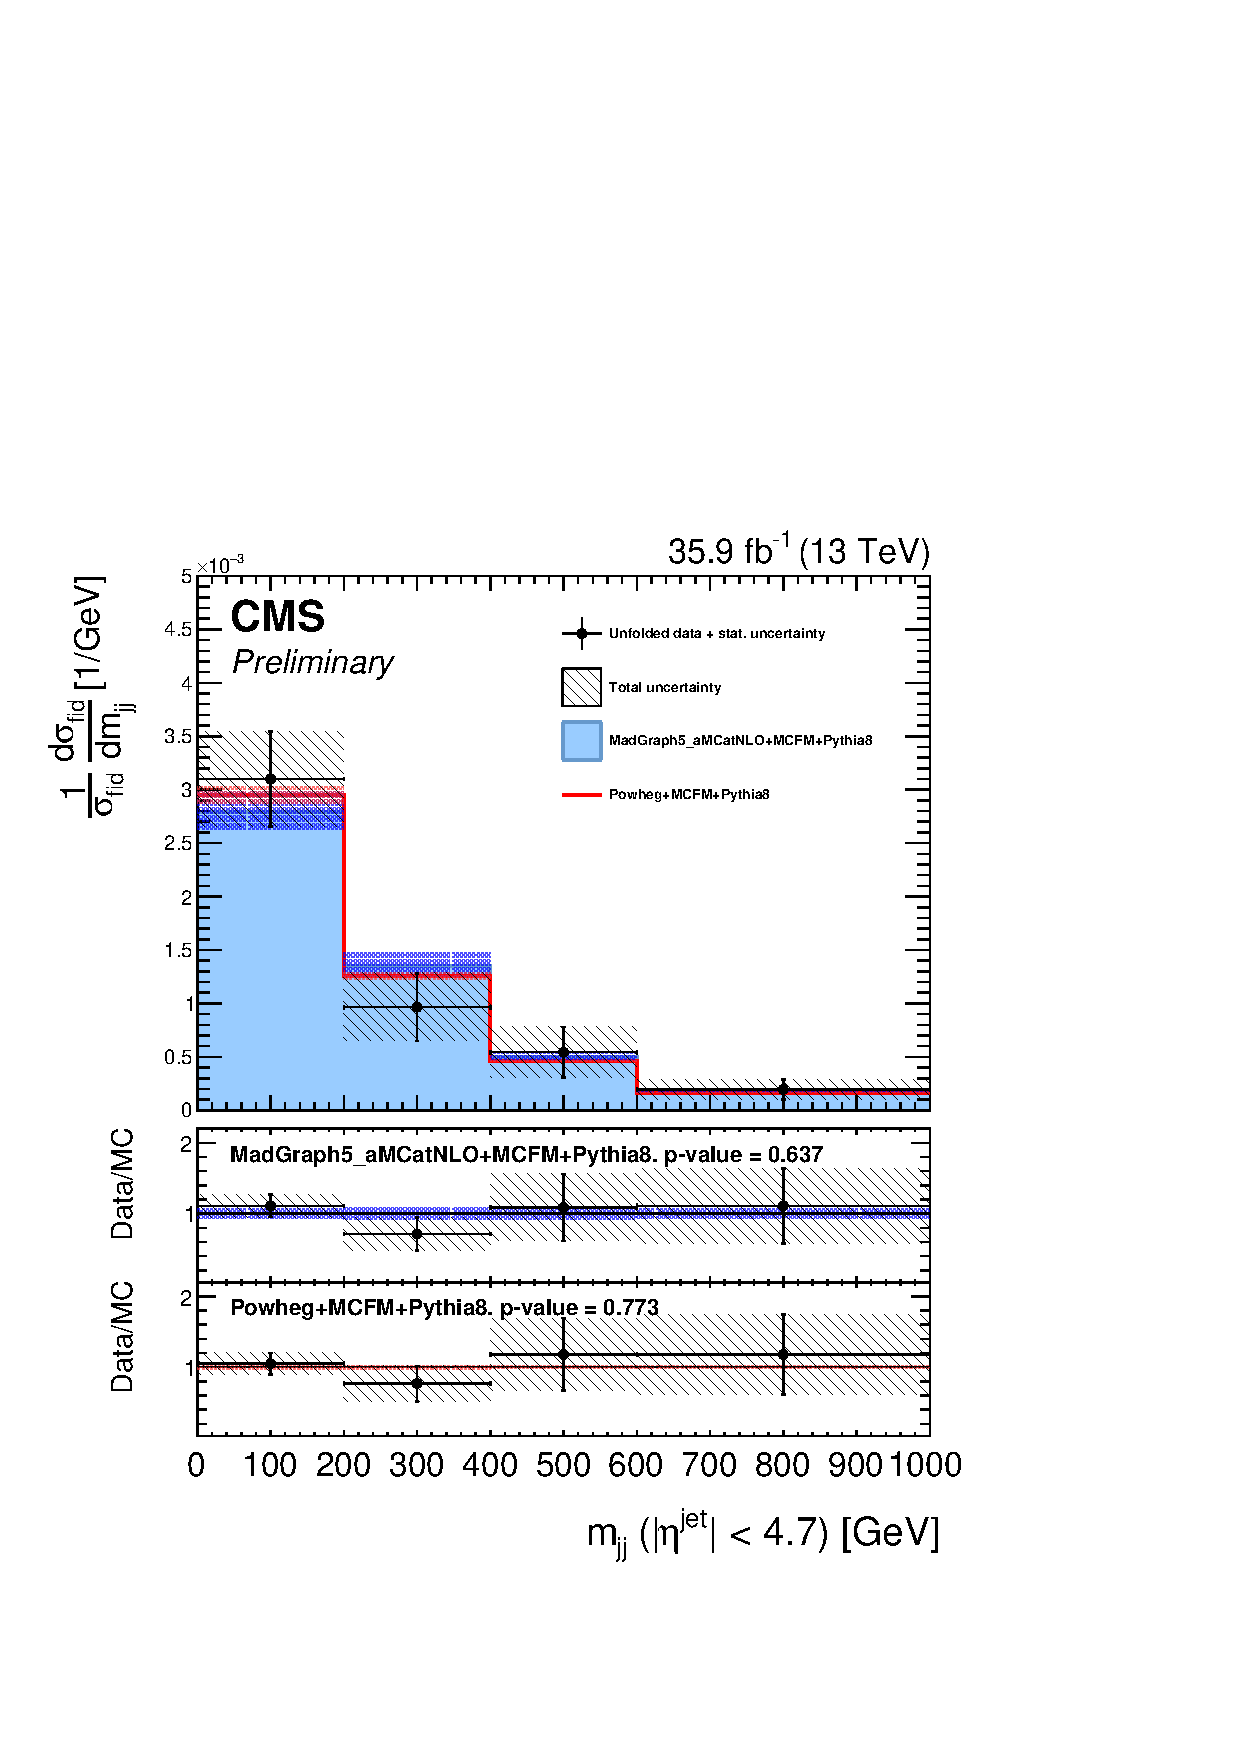
\includegraphics[width=0.88\textwidth]{results/unfold_mjj.pdf}
    \caption[Normalized differential {\ZZ} cross section as a function of dijet invariant mass]{
        The {\ZZ} differential cross section as a function of the invariant mass of the two highest-{\pt} jets $m_{\Pj\Pj}$, including all {\ZZ} events with at least two jets, normalized to the inclusive fiducial cross section.
        Points represent the unfolded data, with vertical bars showing the statistical uncertainty and a hatched band showing the sum in quadrature of the statistical and systematic uncertainties.
        Red and blue histograms represent the {\POWHEG}+{\MCFM} and {\MGAMC}+{\MCFM} predictions, respectively, with bands around each which represent their combined statistical, scale, and PDF uncertainties.
        The lower sections of the plot represents the ratio of the measured cross section to each of the predictions.
      }\label{fig:unfold_mjj}
  \end{center}
\end{figure}

\begin{figure}[htbp]
  \begin{center}
    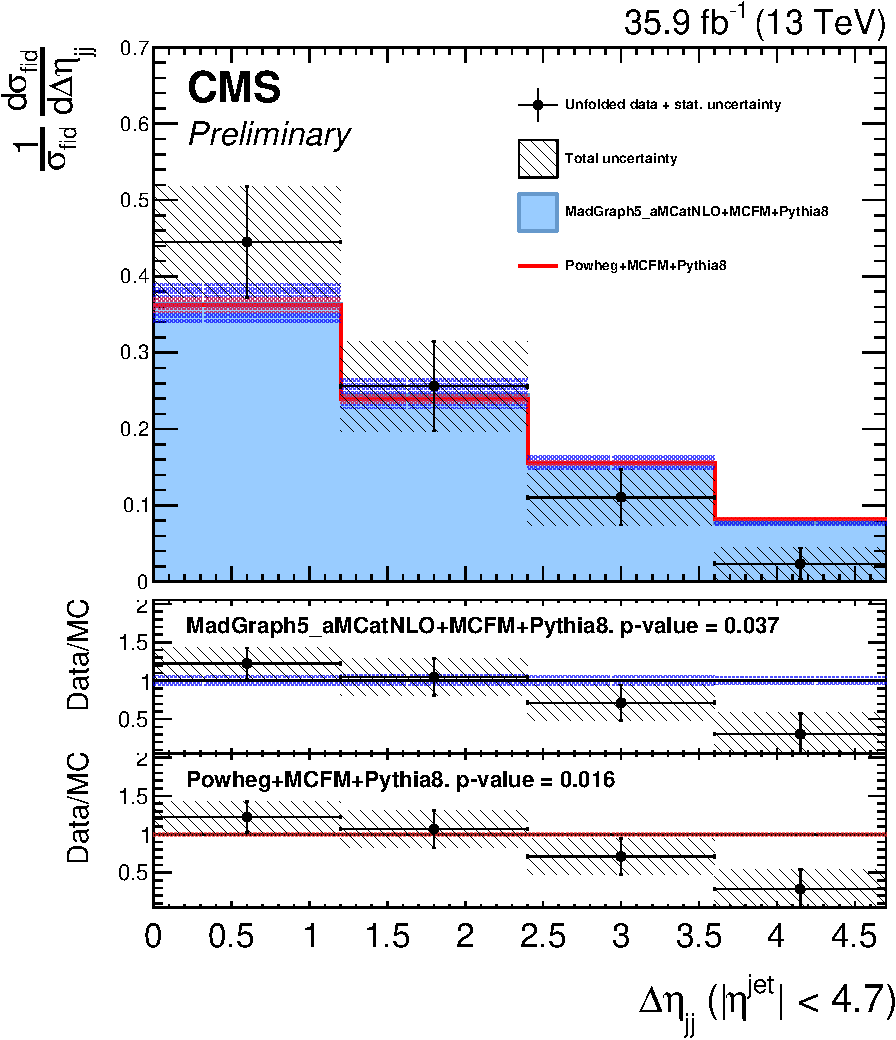
\includegraphics[width=0.88\textwidth]{results/unfold_deltaEtajj.pdf}
    \caption[Normalized differential {\ZZ} cross section as a function of dijet pseudorapidity separation]{
        The {\ZZ} differential cross section as a function of the absolute pseudorapidity separation of the two highest-{\pt} jets $\lvert \Delta \eta_{\Pj\Pj} \rvert$, including all {\ZZ} events with at least two jets, normalized to the inclusive fiducial cross section.
        Points represent the unfolded data, with vertical bars showing the statistical uncertainty and a hatched band showing the sum in quadrature of the statistical and systematic uncertainties.
        Red and blue histograms represent the {\POWHEG}+{\MCFM} and {\MGAMC}+{\MCFM} predictions, respectively, with bands around each which represent their combined statistical, scale, and PDF uncertainties.
        The lower sections of the plot represents the ratio of the measured cross section to each of the predictions.
      }\label{fig:unfold_deltaEtajj}
  \end{center}
\end{figure}

\begin{figure}[htbp]
  \begin{center}
    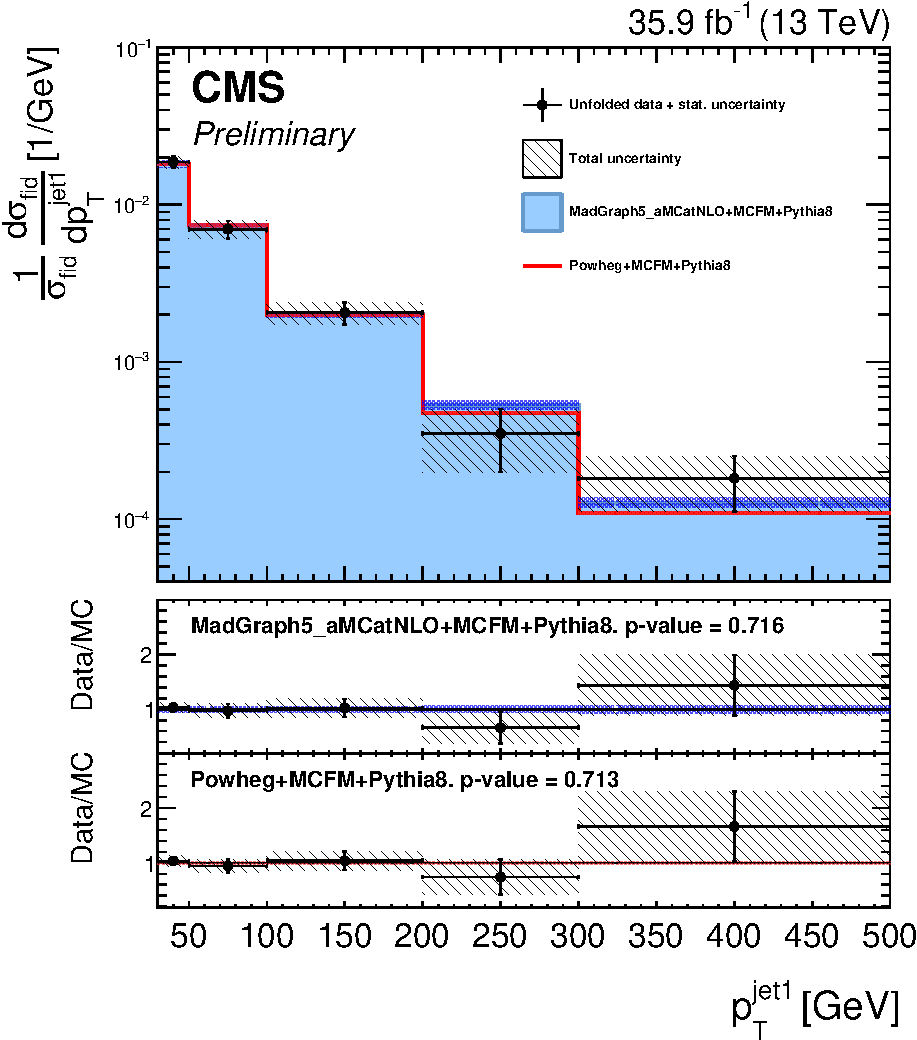
\includegraphics[width=0.495\textwidth]{results/unfold_j1Pt.pdf}
    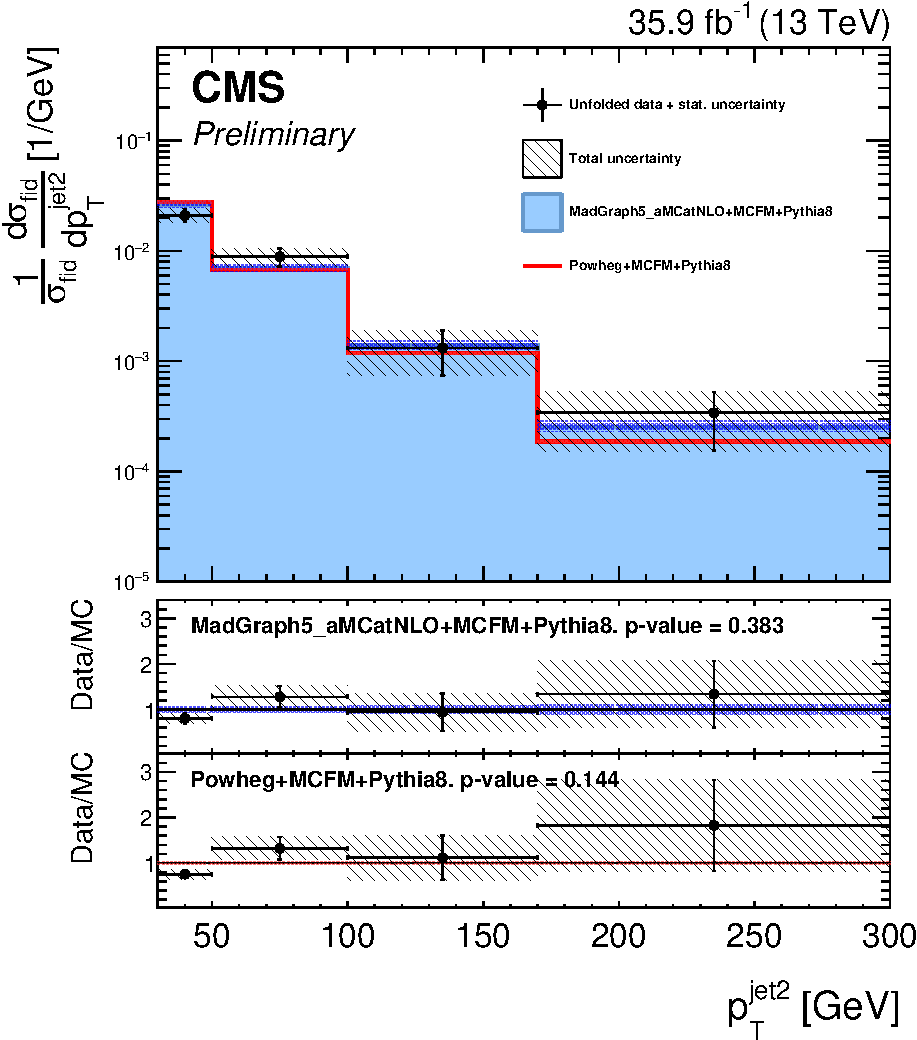
\includegraphics[width=0.495\textwidth]{results/unfold_j2Pt.pdf}
    \caption[Normalized differential {\ZZ} cross sections as functions of leading and subleading jet transverse momentum]{
        The {\ZZ} differential cross section as a function of the leading (left) and subleading (right) jet {\pt}, in {\ZZ} events with at least one jet and at least two jets respectively, normalized to the inclusive fiducial cross section.
        Points represent the unfolded data, with vertical bars showing the statistical uncertainty and a hatched band showing the sum in quadrature of the statistical and systematic uncertainties.
        Red and blue histograms represent the {\POWHEG}+{\MCFM} and {\MGAMC}+{\MCFM} predictions, respectively, with bands around each which represent their combined statistical, scale, and PDF uncertainties.
        The lower sections of the plots represent the ratio of the measured cross section to each of the predictions.
      }\label{fig:unfold_jPt}
  \end{center}
\end{figure}

\begin{figure}[htbp]
  \begin{center}
    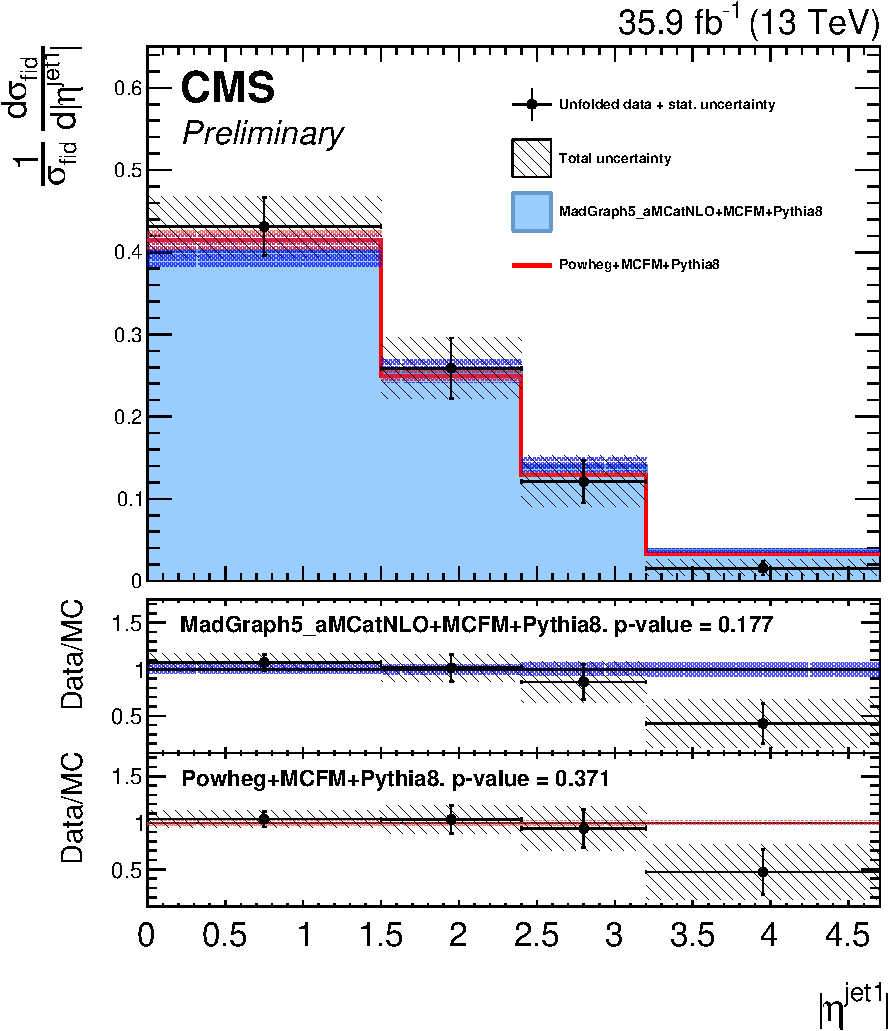
\includegraphics[width=0.495\textwidth]{results/unfold_j1Eta.pdf}
    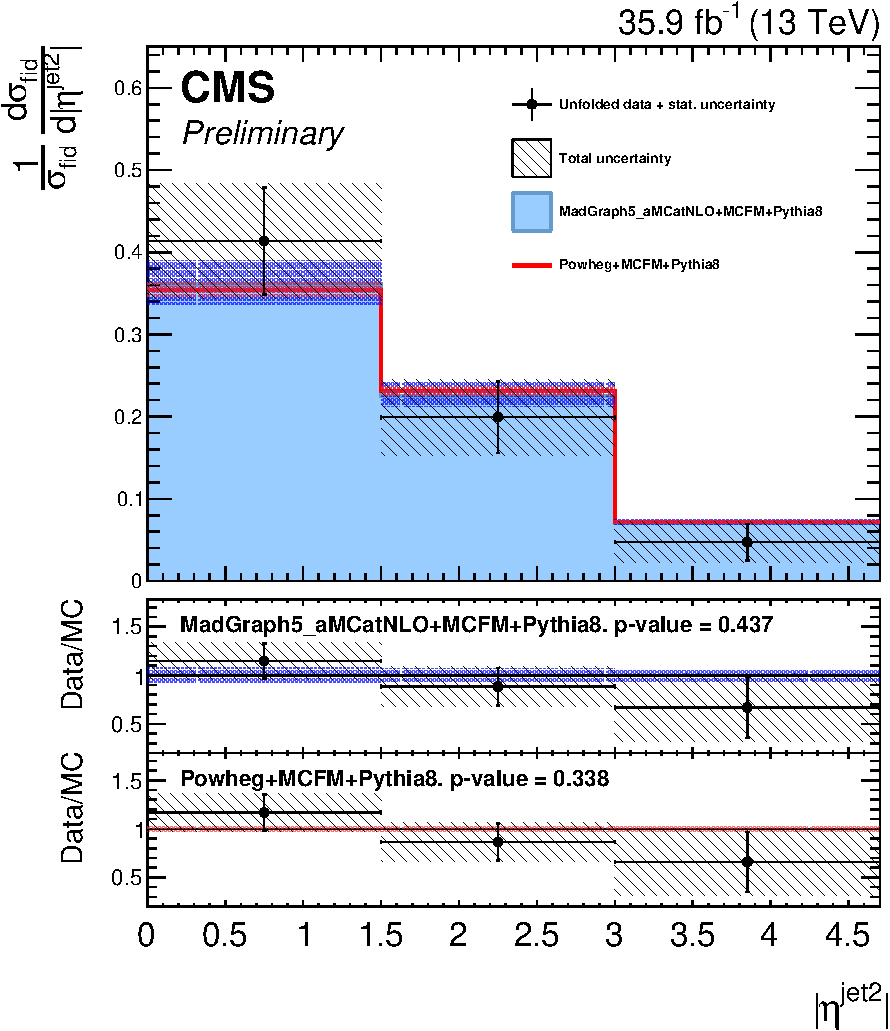
\includegraphics[width=0.495\textwidth]{results/unfold_j2Eta.pdf}
    \caption[Normalized differential {\ZZ} cross sections as functions of leading and subleading jet pseudorapidity]{
        The {\ZZ} differential cross section as a function of the leading (left) and subleading (right) jet {$\eta$}, in {\ZZ} events with at least one jet and at least two jets respectively, normalized to the inclusive fiducial cross section.
        Points represent the unfolded data, with vertical bars showing the statistical uncertainty and a hatched band showing the sum in quadrature of the statistical and systematic uncertainties.
        Red and blue histograms represent the {\POWHEG}+{\MCFM} and {\MGAMC}+{\MCFM} predictions, respectively, with bands around each which represent their combined statistical, scale, and PDF uncertainties.
        The lower sections of the plots represent the ratio of the measured cross section to each of the predictions.
      }\label{fig:unfold_jEta}
  \end{center}
\end{figure}

\begin{figure}[htbp]
  \begin{center}
    \includegraphics[width=0.88\textwidth]{results/unfold_massFull.pdf}
    \caption[Normalized differential four-lepton cross section as a function of four-lepton invariant mass with loosened {\PZ} mass cuts]{
        The four-lepton differential cross section as a function of $m_{4\ell}$ under the full spectrum selections, normalized to the inclusive fiducial cross section.
        Points represent the unfolded data, with vertical bars showing the statistical uncertainty and a grey band showing the sum in quadrature of the statistical and systematic uncertainties.
        Blue and red histograms represent the {\POWHEG}+{\MCFM} and {\MGAMC}+{\MCFM} predictions, respectively, with bands around each which represent their combined statistical, scale, and PDF uncertainties.
        The lower sections of the plot represents the ratio of the measured cross section to each of the predictions.
      }\label{fig:unfold_massFull}
  \end{center}
\end{figure}



\section{Vector Boson Scattering}

Figure~\ref{fig:vbsBDT} shows the output of the GBDT discussed in Section~\ref{sec:vbsSearch} for events in the dijet selection.
The search procedure finds a modest excess of events compatible with VBS {\ZZjj} signal, at the level of 2.7 standard deviations over the null hypothesis of the SM without VBS {\ZZ} production.
The expected significance is 1.6 standard deviations.
This corresponds to a VBS fiducial cross section of
\begin{equation}
  \sigma_\text{fid}(\pp \to \PZ\PZ\Pj\Pj\text{(EWK)} \to 4\ell\Pj\Pj) = 0.40^{+0.21}_{-0.16} \stat ^{+0.13}_{-0.09} \syst \unit{fb},
\end{equation}
which is consistent with the SM prediction of $0.29^{+0.02}_{-0.03} \unit{fb}$.


\begin{figure}[htbp]
  \begin{center}
    \includegraphics[width=0.75\textwidth]{results/BDT_someVBS.pdf}
    \caption[VBS signal extraction GBDT output]{
        Output distribution of the VBS signal extraction GBDT, for events in the dijet selection.
        Points represent data, with statistical uncertainty bars.
        The stack of filled histograms represents the SM signal prediction and background estimate.
      }\label{fig:vbsBDT}
  \end{center}
\end{figure}



\section{Anomalous Coupling Limits}

The {\ZZ} invariant mass is shown in Fig.~\ref{fig:aTGC} for all events in the on-shell selection, with two example distributions shown for potential scenarios with nonzero aTGCs, one of which sets $f_5^\Pa = 0.0019$ and $f_5^\PZ = 0.0015$, and the other $f_4^\Pa = 0.0019$ and $f_4^\PZ = 0.0015$.
The limit setting procedure described in Section~\ref{sec:aGCSearch} is applied to each aTGC parameter, with all other couplings fixed to their SM values, to yield one-dimensional 95\% CL limits,
\begin{equation}\label{eq:aTGC1D}
  \begin{aligned}
  & -0.0012 < f_4^\PZ < 0.0010   ,  & -0.0010 < f_5^\PZ < 0.0013 , \\
  & -0.0012 < f_4^\Pa < 0.0013   ,  & -0.0012 < f_5^\Pa < 0.0013 .
  \end{aligned}
\end{equation}
These results improve the previous CMS limits, which were the most stringent set previously, by factors of 2--3~\cite{Khachatryan:2015pba} and are the most stringent limits to date on the parameters in question.
Recent preliminary limits from ATLAS using {13\TeV} data are 50--80\% looser~\cite{ATLAS:2017eyk}.
Two-dimensional limits are set in the $f_4^\Pa$-$f_4^\PZ$ and $f_5^\Pa$-$f_5^\PZ$ planes, holding all other parameters to the SM values in each calculation.
One- and two-dimensional 95\% CL limits are shown in Fig.~\ref{fig:aTGC2D}.


\begin{figure}[htbp]
  \begin{center}
    \includegraphics[width=0.75\textwidth]{results/zzMass_aTGC.pdf}
    \caption[{\ZZ} invariant mass distribution with example aTGC working points]{
        Distribution of {\ZZ} invariant mass for all events in the on-shell selection.
        Points represent data, with statistical uncertainty bars.
        The stack of filled histograms represents the SM signal prediction and background estimate.
        The unfilled histograms represent two example {\SHERPA} predictions for nonzero aTGC hypotheses (dashed) and the {\SHERPA} SM prediction (solid), included to illustrate the shape differences between the {\SHERPA} and {\POWHEG}+{\MCFM} SM predictions.
        The {\SHERPA} distributions are normalized such that the SM prediction's total yield matches that of the other generators.
        The last bin includes the overflow contributions from events at masses above {1.2\TeV}.
      }\label{fig:aTGC}
  \end{center}
\end{figure}

\begin{figure}[htbp]
  \begin{center}
    \includegraphics[width=0.495\textwidth]{results/limits2D_f4.pdf}
    \includegraphics[width=0.495\textwidth]{results/limits2D_f5.pdf}
    \caption[Asymptotic one- and two-dimensional aTGC limits at 95\% confidence level]{
        Two-dimensional observed 95\% CL limits (solid contour) and expected 68 and 95\% CL limits (dashed contours) in the $f_4^\Pa$-$f_4^\PZ$ (left) and $f_5^\Pa$-$f_5^\PZ$ (right) planes.
        The regions outside the contours are excluded at the corresponding confidence level.
        The dot is the point of maximum likelihood in the two-dimensional fits.
        Solid, straight lines at the center show the observed one-dimensional 95\% CL limits for $f_{4,5}^\Pa$ (horizontal) and $f_{4,5}^\PZ$ (vertical).
        No form factor is used.
      }\label{fig:aTGC2D}
  \end{center}
\end{figure}


No unitarizing form factor (c.f.\ Section~\ref{sec:aTGCTheory}) is applied when calculating the limits of Eq.~(\ref{eq:aTGC1D}).
One way to enforce unitarity without a form factor would be to restrict the maximum {\ZZ} invariant mass used, and set the limits considering only events with $m_{\ZZ}$ below some cutoff.
The limits would then depend on the cutoff chosen, converging to the nonunitary limits when the cutoff is larger than the energies accessible in the experiment.
The limit computations are repeated with multiple cutoff values, and the resulting expected and observed limits are shown in Fig.~\ref{fig:aTGCCutoff} as a function of the maximum $m_{\ZZ}$ used.


\begin{figure}[htbp]
  \begin{center}
    \includegraphics[width=0.48\textwidth]{results/limits1DVsCutoff_g4.pdf}
    \includegraphics[width=0.48\textwidth]{results/limits1DVsCutoff_z4.pdf} \\
    \includegraphics[width=0.48\textwidth]{results/limits1DVsCutoff_g5.pdf}
    \includegraphics[width=0.48\textwidth]{results/limits1DVsCutoff_z5.pdf}
    \caption[One-dimensional aTGC limits as a function of the maximum {\ZZ} invariant mass used in the calculation]{
        Expected and observed one-dimensional limits on the four aTGC parameters, as functions of the $m_{\ZZ}$ cutoff used to enforce unitarity.
        No form factor is used.
      }\label{fig:aTGCCutoff}
  \end{center}
\end{figure}

The aQGC search proceeds the same way, but using events in the dijet selection.
The observable used for limit setting is again $m_{\ZZ}$, which is shown for these events in Fig.~\ref{fig:aQGC} along with two example distributions for scenarios with nonzero aQGCs, one with $f_\text{T8}/\Lambda^4 = 1\TeVns^{-4}$, the other with $f_\text{T9}/\Lambda^4 = 2\TeVns^{-4}$.
In the aQGC search, a unitarity bound is imposed, chosen with \textsc{vbfnlo}~\cite{Arnold:2008rz} to be the value of $m_{\ZZ}$ at which the scattering amplitude would violate unitarity if the aQGC parameter in question were set to its 95\% CL limit value.
While limits are set for each parameter, all other parameters and their unitarity bounds are set to zero.
The observed 95\% CL limits on the coefficients of the effective field theory operators coverning {\ZZjj} production are
\begin{equation}\label{eq:aQGC1D}
  \begin{aligned}
    &-0.46  &<& \quad  f_\text{T0} / \Lambda^4  &<&  \quad  0.44  & \TeV^{-4}, \\
    &-0.61  &<& \quad  f_\text{T1} / \Lambda^4  &<&  \quad  0.61  & \TeV^{-4}, \\
    &-1.2   &<& \quad  f_\text{T2} / \Lambda^4  &<&  \quad  1.2   & \TeV^{-4}, \\
    &-0.84  &<& \quad  f_\text{T8} / \Lambda^4  &<&  \quad  0.84  & \TeV^{-4}, \\
    &-1.8   &<& \quad  f_\text{T9} / \Lambda^4  &<&  \quad  1.8   & \TeV^{-4}.
  \end{aligned}
\end{equation}
These are the most stringent constraints to date on all five parameters, improving on the previous best by factors of 2--8 (see Section~\ref{sec:aTGCLit}).
This is the first time any of them have been measured in the {\ZZjj} channel.


\begin{figure}[htbp]
  \begin{center}
    \includegraphics[width=0.75\textwidth]{results/zzMass_aQGC.pdf}
    \caption[{\ZZ} invariant mass distribution for dijet events, with example aQGC working points]{
        Distribution of {\ZZ} invariant mass for events in the dijet selection.
        Points represent data, with statistical uncertainty bars.
        The stack of filled histograms represents the SM signal prediction and background estimate.
        The unfilled histograms represent two example {\MGAMC} distributions for nonzero aQGC hypotheses.
        The last bin includes the overflow contributions from events at masses above {1.4\TeV}.
      }\label{fig:aQGC}
  \end{center}
\end{figure}

\chapter{Conclusions}
Definitive



% \appendix
% \include{appendix_yields}
% \include{appendix_acceff}

%\bibliographystyle{plain}

%\bibliographystyle{unsrt}
%\bibliographystyle{ieeetr}
%\bibliographystyle{IEEEtran}

%\bibliography{backmatter/bibliography.bib}

\SingleSpace{}
\setlength{\bibitemsep}{\onelineskip}
\printbibliography{}

\end{document}
